%%%%%%%%%%%%%%%%%%%%%%%%
% Sample use of the infthesis class to prepare an MSc thesis.
% This can be used as a template to produce your own thesis.
% Date: June 2019
%
%
% The first line specifies style options for taught MSc.
% You should add a final option specifying your degree.
% *Do not* change or add any other options.
%
% So, pick one of the following:
% \documentclass[msc,deptreport,adi]{infthesis}     % Adv Design Inf
% \documentclass[msc,deptreport,ai]{infthesis}      % AI
% \documentclass[msc,deptreport,cogsci]{infthesis}  % Cognitive Sci
% \documentclass[msc,deptreport,cs]{infthesis}      % Computer Sci
% \documentclass[msc,deptreport,cyber]{infthesis}   % Cyber Sec
% \documentclass[msc,deptreport,datasci]{infthesis} % Data Sci
% \documentclass[msc,deptreport,di]{infthesis}      % Design Inf
% \documentclass[msc,deptreport,inf]{infthesis}     % Informatics
%%%%%%%%%%%%%%%%%%%%%%%%

\documentclass[msc,deptreport.inf]{infthesis} % Do not change except to add your degree (see above).

% maths
\usepackage{amsmath}
\usepackage{amsfonts}
\usepackage{amssymb}
\newcommand{\matr}[1]{\mathbf{#1}}
\newcommand{\bgreek}[1]{\boldsymbol{#1}}
\newcommand{\R}{\mathbb R}
\newcommand{\E}{\mathbb E}
\newcommand{\V}{\mathbb V}
\newcommand{\N}{\mathbb N}
\newcommand{\D}{\mathbb D}
\newcommand{\diag}{\mathop{\mathrm{diag}}}
\newcommand{\tr}{\mathop{\mathrm{Tr}}}

% algorithms
\usepackage{algorithm, algpseudocode}
\renewcommand{\algorithmicrequire}{\textbf{Input:}}
\renewcommand{\algorithmicensure}{\textbf{Output:}}

% graphics
\usepackage{graphicx}
\usepackage{subfig}


\begin{document}
\begin{preliminary}

\title{Extending the Bayesian Deep Learning Method MultiSWAG}

\author{Scott Brownlie}

\abstract{
  This skeleton demonstrates how to use the \texttt{infthesis} style
  for MSc dissertations in Artificial Intelligence, Cognitive Science,
  Computer Science, Data Science, and Informatics. It also emphasises
  the page limit, and that you must not deviate from the required
  style.  The file \texttt{skeleton.tex} generates this document and
  can be used as a starting point for your thesis. The abstract should
  summarise your report and fit in the space on the first page.
}

\maketitle

\section*{Acknowledgements}
Any acknowledgements go here.

\tableofcontents
\end{preliminary}


\chapter{Introduction}

The preliminary material of your report should contain:
\begin{itemize}
\item
The title page.
\item
An abstract page.
\item
Optionally an acknowledgements page.
\item
The table of contents.
\end{itemize}

As in this example \texttt{skeleton.tex}, the above material should be
included between:
\begin{verbatim}
\begin{preliminary}
    ...
\end{preliminary}
\end{verbatim}
This style file uses roman numeral page numbers for the preliminary material.

The main content of the dissertation, starting with the first chapter,
starts with page~1. \emph{\textbf{The main content must not go beyond page~40.}}

The report then contains a bibliography and any appendices, which may go beyond
page~40. The appendices are only for any supporting material that's important to
go on record. However, you cannot assume markers of dissertations will read them.

You may not change the dissertation format (e.g., reduce the font
size, change the margins, or reduce the line spacing from the default
1.5 spacing). Over length or incorrectly-formatted dissertations will
not be accepted and you would have to modify your dissertation and
resubmit.  You cannot assume we will check your submission before the
final deadline and if it requires resubmission after the deadline to
conform to the page and style requirements you will be subject to the
usual late penalties based on your final submission time.

%\section{Using Sections}
%
%Divide your chapters into sub-parts as appropriate.
%
%\section{Citations}
%
%Citations (such as \cite{P1} or \cite{P2}) can be generated using
%\texttt{BibTeX}. For more advanced usage, the \texttt{natbib} package is
%recommended. You could also consider the newer \texttt{biblatex} system.
%
%These examples use a numerical citation style. You may also use
%(Author, Date) format if you prefer.
%
%\chapter{Your next chapter}
%
%A dissertation usually contains several chapters.


\chapter{Background}\label{ch:background}

\section{Factor Analysis}\label{sec:fa}

Factor analysis (FA) is a latent variable model which generates observations $\theta \in \R^D$ as follows. First, a latent vector $\matr{h} \in \R^K$, for some $K < D$, is sampled from $p(\matr{h}) = \mathcal{N}(\matr{0}, \matr{I})$. Next, $\matr{h}$ is transformed onto a $K$-dimensional linear subspace of $\R^D$ by left-multiplying it by a \emph{factor loading} matrix $\matr{F} \in \R^{D \times K}$. The origin of this subspace is then shifted by adding a bias term $\matr{c} \in \R^D$. Finally, the data is perturbed by adding some zero mean Gaussian noise $\epsilon \in \R^D$ sampled from $\mathcal{N}(\matr{0}, \Psi)$, where $\Psi$ is a $D\times D$ diagonal matrix \cite{barber2007}. Putting all this together, an observation $\theta \in \R^D$ is generated according to 
\begin{equation}\label{eqn:fa_model}
	\theta = \matr{Fh} + \matr{c} + \epsilon.
\end{equation}
In the context of this thesis, an observation $\theta$ is the parameter vector of a neural network. 

It follows that, given $\matr{h}$, the observations $\theta$ are Gaussian distributed with mean $\matr{Fh} + \matr{c}$ and covariance $\Psi$ \cite{barber2007}. Formally,
\begin{equation}\label{eqn:fa_cond_dist}
	p(\theta | \matr{h}) 
	= \mathcal{N}\Big( \matr{Fh} + \matr{c}, \Psi \Big)
	= \frac{1}{\sqrt{(2\pi)^D |\Psi|}} 
	\exp \Big(-\frac{1}{2} (\theta - \matr{Fh} - \matr{c})^\intercal \Psi^{-1} (\theta - \matr{Fh} - \matr{c})\Big),
\end{equation}
where $|\Psi|$ is the \emph{determinant} of $\Psi$. From \cite{barber2007}, integrating $p(\theta | \matr{h})$ over $\matr{h}$ gives the marginal distribution
\begin{equation}\label{eqn:fa_marginal_dist}
	p(\theta) = \mathcal{N}\big(\matr{c}, \matr{FF}^{\intercal} + \Psi\big).
\end{equation}
The parameters of the model are $\matr{c}, \matr{F}$ and $\Psi$. The value of $\matr{c}$ which maximises the likelihood of the observed data is the empirical mean of the observations \cite{barber2007}, which in this case is $\theta_{\text{SWA}}$. 
%By substituting $\matr{c} = \theta_{\text{SWA}}$ into $p(\theta)$, the distribution in (\ref{eqn:fa_dist}) is obtained. 
Having set the bias term, an expectation-maximisation (EM) or singular value decomposition (SVD) algorithm can find the maximum likelihood estimates of $\matr{F}$ and $\Psi$ \cite{barber2007}. However, both methods require storing all the observations in memory, making them impractical for high-dimensional data, such as the parameter vectors of deep neural networks. Two alternative online algorithms are presented in Chapter \ref{ch:online_fa}.

\section{Bayesian Linear Regression}\label{sec:bayesian_lr}

A linear regression model is a mapping from vector inputs $\matr{x} \in \R^D$ to scalar outputs $y \in \R$ via an affine transformation. Given a set of observed input-output pairs, $\mathcal{D} = \{(\matr{x}_n, y_n)\}_{n=1}^{N}$, it is assumed that each output is generated according to 
\begin{equation}\label{eqn:linear_regression}
	y_n = \theta^\intercal \matr{x}_n + \epsilon
\end{equation}
for some unknown $\theta \in \R^D$. The underlying signal, $\theta^\intercal \matr{x}_n$, is corrupted by additive noise, 
\begin{equation}
	\epsilon \sim \mathcal{N}(0, \sigma^2), 
\end{equation}
for some $\sigma > 0$ \cite{barber2007}. The model is often written with an explicit bias term, but this can be absorbed into $\theta$ by adding a constant of one to the input, leading to the expression in Equation (\ref{eqn:linear_regression}).

\subsection{Computing the Posterior}

Due to the additive noise, each $y_n$ is a random variable, conditioned on $\matr{x}_n$ and $\theta$. Since $\epsilon$ is Gaussian distributed, the conditional pdf of $y_n$ is 
\begin{equation}\label{eqn:linear_regression_pdf}
	p(y_n | \theta, \matr{x}_n) 
	= \mathcal{N}\big(\theta^\intercal \matr{x}_n, \sigma^2\big)
	= \frac{1}{\sqrt{2\pi \sigma^2}} \exp\Big(-\frac{1}{2\sigma^2} \big(y_n - \theta^\intercal \matr{x}_n \big)^2\Big).
\end{equation}
Assuming that the observations in $\mathcal{D}$ are independent and identically distributed (iid), the log-likelihood of $\theta$ having generated the data is 
\begin{align}\label{eqn:linear_regression_log_likelihood}
\begin{split}
	\log p(\mathcal{D} | \theta) 
	& = \sum_{n=1}^N \big[ \log p(y_n | \theta, \matr{x}_n)  + \log p(\matr{x}_n) \big] \\
	& = \sum_{n=1}^N \Big[ -\frac{1}{2} \log 2\pi \sigma^2 - \frac{1}{2\sigma^2} \big(y_n - \theta^\intercal \matr{x}_n \big)^2 \Big]
	+ \sum_{n=1}^N \log p(\matr{x}_n) \\
	& = - \frac{1}{2 \sigma^2} \sum_{n=1}^N \big(y_n - \theta^\intercal \matr{x}_n \big)^2 
	- \frac{N}{2} \log \sigma^2
	- \frac{N}{2} \log 2\pi
	+ \sum_{n=1}^N \log p(\matr{x}_n) \\
	& = - \frac{\beta}{2} \sum_{n=1}^N \big(y_n - \theta^\intercal \matr{x}_n \big)^2 
	+ \frac{N}{2} \log \beta
	+ \text{constant},
\end{split}
\end{align}
where $\beta = \frac{1}{\sigma^2}$ \cite{barber2007}. In Bayesian linear regression, a prior distribution for $\theta$ is also specified. A common choice  is 
\begin{equation}\label{eqn:linear_regression_prior}
	p(\theta) 
	= \mathcal{N}\big(\matr{0}, \alpha^{-1} \matr{I} \big)
	= \Big(\frac{\alpha}{2\pi}\Big)^{\frac{D}{2}} \exp\Big(-\frac{\alpha}{2} \theta^\intercal \theta \Big)
\end{equation}
for some $\alpha > 0$, which is a hyperparameter known as the \emph{precision} \cite{barber2007}. Applying the logarithm, 
\begin{align}\label{eqn:linear_regression_log_prior}
\begin{split}
	\log p(\theta) 
	& = \frac{D}{2} \log \frac{\alpha}{2\pi} - \frac{\alpha}{2} \theta^\intercal \theta \\
	& = -\frac{\alpha}{2} \theta^\intercal \theta + \frac{D}{2} \log \alpha + \text{constant}.
\end{split}
\end{align}
Now, using Bayes' rule and Equation (\ref{eqn:linear_regression_log_likelihood}) and Equation (\ref{eqn:linear_regression_log_prior}), it follows that the log-posterior distribution of $\theta$ for fixed $\alpha$ and $\beta$ is 
\begin{align}\label{eqn:linear_regression_log_posterior}
\begin{split}
	\log p(\theta | \mathcal{D}) 
	& = \log \frac{p(\mathcal{D} | \theta) p(\theta)}{p(\mathcal{D})} \\
	& = \log p(\mathcal{D} | \theta) + \log p(\theta) - \log p(\mathcal{D}) \\
	& = -\frac{\beta}{2} \sum_{n=1}^N \big(y_n - \theta^\intercal \matr{x}_n \big)^2 
	-\frac{\alpha}{2} \theta^\intercal \theta 
	+ \text{constant} \\
	& = -\frac{\beta}{2} \sum_{n=1}^N\big( y_n^2 - 2 y_n \theta^\intercal \matr{x}_n + (\theta^\intercal \matr{x}_n)^2 \big)
	-\frac{\alpha}{2} \theta^\intercal \theta
	+ \text{constant} \\
	& = -\frac{\beta}{2} \sum_{n=1}^N y_n^2
	+ \beta \sum_{n=1}^N y_n \theta^\intercal \matr{x}_n
	-\frac{\beta}{2} \sum_{n=1}^N \theta^\intercal \matr{x}_n \matr{x}_n^\intercal \theta
	-\frac{\alpha}{2} \theta^\intercal \theta
	+ \text{constant} \\
	& = \Big(\beta \sum_{n=1}^N y_n \matr{x}_n \Big)^\intercal \theta 
	-\frac{1}{2} \theta^\intercal \Big( \alpha \matr{I} + \beta \sum_{n=1}^N \matr{x}_n \matr{x}_n^\intercal \Big) \theta 
	+ \text{constant} \\
	& = \matr{b}^\intercal \theta 
	- \frac{1}{2} \theta^\intercal \matr{A} \theta 
	+ \text{constant},
\end{split}
\end{align}
where 
\begin{equation}\label{eqn:linear_model_A_and_b}
	\matr{A} = \alpha \matr{I} + \beta \sum_{n=1}^N \matr{x}_n \matr{x}_n^\intercal
	\quad \text{and} \quad 
	\matr{b} = \beta \sum_{n=1}^N y_n \matr{x}_n.
\end{equation}
Now, using a result from \cite{barber2007} to complete the square of Equation (\ref{eqn:linear_regression_log_posterior}),
\begin{align}
\begin{split}
	\log p(\theta | \mathcal{D}) 
	& = -\frac{1}{2} \big(\theta - \matr{A}^{-1} \matr{b} \big)^\intercal \matr{A} \big(\theta - \matr{A}^{-1} \matr{b} \big)
	+ \frac{1}{2} \matr{b}^\intercal \matr{A}^{-1} \matr{b}
	+ \text{constant} \\
	& = -\frac{1}{2} \big(\theta - \matr{A}^{-1} \matr{b} \big)^\intercal \matr{A} \big(\theta - \matr{A}^{-1} \matr{b} \big)
	+ \text{constant} \\
	& = -\frac{1}{2} \big(\theta - \matr{m} \big)^\intercal \matr{S}^{-1} \big(\theta - \matr{m} \big)
	+ \text{constant},
\end{split}
\end{align}
where
\begin{equation}\label{eqn:linear_regression_posterior_params}
	\matr{m} = \matr{A}^{-1} \matr{b}
	\quad \text{and} \quad 
	\matr{S} = \matr{A}^{-1}.
\end{equation}
Hence, the posterior distribution of $\theta$ is 
\begin{align}\label{eqn:linear_regression_posterior}
\begin{split}
	p(\theta | \mathcal{D}) = \mathcal{N}(\matr{m}, \matr{S}).
\end{split}
\end{align}


\section{Variational Inference}\label{sec:vi}

For linear regression, computing the posterior in Equation (\ref{eqn:linear_regression_posterior}) is possible because the log-likelihood, $p(\mathcal{D} | \theta)$, is a quadratic expression of $\theta$. However, when $\theta$ is the parameter vector of a neural network with even a single non-linear hidden layer, the log-likelihood is not so simple and the posterior cannot be written in closed form. Instead, the marginal likelihood, $p(\mathcal{D}) = \int_\theta p(\mathcal{D} | \theta) p(\theta)$, must be evaluated, which is intractable for high-dimensional $\theta$. 

An alternative strategy is to approximate the posterior directly with a Gaussian distribution $q(\theta) = \mathcal{N}(\mu, \Sigma)$, where the parameters $\mu$ and $\Sigma$ are chosen to minimise some measure of dissimilarity between $q(\theta)$ and $p(\theta | \mathcal{D})$. Because $q(\theta)$ is essentially a variable in an optimisation procedure, this approach is known as \emph{variational inference} (VI) \cite{barber2007}. A common measure of dissimilarity between two distributions is the Kullback-Leibler (KL) divergence \cite{barber2007}, which in this case is
\begin{align}
\begin{split}
	\D_{KL}[q(\theta) \Vert p(\theta | \mathcal{D})] 
	& = \E_{q(\theta)} \Big[\log \frac{q(\theta)}{p(\theta | \mathcal{D})}\Big] \\
	& = \E_{q(\theta)} \Big[\log \frac{q(\theta) p(\mathcal{D})}{p(\mathcal{D} | \theta) p(\theta)}\Big] \\
	& = \E_{q(\theta)} [\log q(\theta) - \log p(\theta) - \log p(\mathcal{D} | \theta) + \log p(\mathcal{D})].
\end{split}
\end{align}
Since $p(\mathcal{D})$ is a constant, it can be ignored and the optimal distribution can be obtained by solving 
\begin{equation}\label{eqn:vi_objective}
	\min_{\mu, \Sigma} \big[ \E_{q(\theta)} [\log q(\theta)] - \E_{q(\theta)} [\log p(\theta) ] - \E_{q(\theta)} [\log p(\mathcal{D} | \theta)] \big].
\end{equation}
One way to do this is by using a stochastic gradient algorithm, which approximates the true gradient of the objective function with Monte Carlo estimates of the form
\begin{equation}\label{eqn:vi_derivatives}
	\frac{1}{ML} \sum_{m=1}^M \sum_{l=1}^L \big[ \nabla_{\mu, \Sigma} \log q(\theta_l) - \nabla_{\mu, \Sigma} \log p(\theta_l) -  \nabla_{\mu, \Sigma} \log p(y_m | \matr{x}_m, \theta_l) \big],
\end{equation}
where $\{(y_m, \matr{x}_m)\}_{m=1}^M$ is a batch of observed data sampled from $\mathcal{D}$ and $\theta_l \sim \mathcal{N}(\mu, \Sigma)$. Normally it would not be possible to compute partial derivatives with respect to $\mu$ and $\Sigma$, given that they only take part via the random sampling operation. However, this can in fact be done by using the \emph{re-parameterisation trick} \cite{goodfellow2016}. Instead of sampling from $\mathcal{N}(\mu, \Sigma)$ directly, a random variable $\matr{z}_l$ is sampled from $\mathcal{N}(\matr{0}, \matr{I})$ and then transformed to $\theta_l$ via a deterministic operation involving $\mu$ and $\Sigma$. This simple trick means that Equation (\ref{eqn:vi_derivatives}) can be evaluated and used in conjunction with SGD or any of its variants to optimise the objective in Equation (\ref{eqn:vi_objective}). This is the idea behind the \emph{auto-encoding variational Bayes} algorithm \cite{kingma2013}.


%\section{Gaussian Processes}\label{sec:gps}
%
%
%As in Section \ref{sec:bayesian_lr}, let $\mathcal{D} = \{(\matr{x}_n, y_n)\}_{n=1}^{N}$ be a set of training examples, where each $\matr{x}_n \in \R^D$ and $y_n \in \R$. Considering only the training set for now, a function $f$ can be specified by its values $\{f_n =  f(\matr{x}_n)\}_{n=1}^{N}$. Letting $\matr{f} = (f_1, \dots, f_N)^\intercal$, the function $f$ can be seen to generate a sample from a multivariate distribution. If this distribution is constrained to be Gaussian, then it is completely specified by the pdf
%\begin{equation}
%	p(\matr{f}) = \mathcal{N}(\mu, \Sigma)
%\end{equation}
%with parameters $\mu \in \R^D$ and $\Sigma \in \R^{D \times D}$. This is an example of a Gaussian process (GP), which is defined as a collection of random variables such that any finite number of the variables are jointly Gaussian \cite{rasmussen2006}. In this case, the finite subset contains the function values of $\{\matr{x}_n\}_{n=1}^{N}$, but any other set of inputs $\matr{x} \in \R^D$ would similarly give rise to a multivariate Gaussian distribution. 
%
%The distribution $p(\matr{f})$ can be used as a prior on the function values of the training inputs before observing the outputs $y_n$. In the absence of domain knowledge about which function values are possible, a sensible choice for the prior mean is $\mu = \matr{0} \in \R^D$. By definition, the covariance matrix $\Sigma$ must be positive semi-definite. If $\Sigma$ was diagonal, function values $f_i$ and $f_j$, $i, j \in \{1, \dots, N\}$, would be independent, irrespective of how close $\matr{x}_i$ is to $\matr{x}_j$. This would lead to extremely noisy functions. To encourage smoothness, it is preferable to define a covariance matrix which assigns greater dependance between function values of nearby inputs. One way to generate covariance matrices with this property is by using the \emph{squared exponential kernel} function \cite{rasmussen2006}. Formally,
% \begin{equation}
%	\Sigma_{i, j} = k(\matr{x}_i, \matr{x}_j) = \exp \Big( -\frac{1}{2} |\matr{x}_i - \matr{x}_j|^2 \Big).
%\end{equation}
%Different \emph{kernel} functions $k(\cdot, \cdot)$ give rise to different covariance matrices, and hence, different priors on the function values. 
%
%To simplify the notation in what follows, let $\matr{X} \in \R^{N\times D}$ be formed by stacking $\matr{x}_1^\intercal,\dots,\matr{x}_N^\intercal$ in the rows of a matrix. Then the zero mean prior can be written as 
%\begin{equation}
%	p(\matr{f}) = \mathcal{N}(\matr{0}, K(\matr{X}, \matr{X})),
%\end{equation}
%where $K(\matr{A}, \matr{B})$, for $\matr{A} \in \R^{N\times D}$ and $\matr{B} \in \R^{M\times D}$, is shorthand from \cite{rasmussen2006} for the $N \times M$ matrix with elements
%\begin{equation}
%	K(\matr{A}, \matr{B})_{i, j} = k(\matr{a}_i, \matr{b}_j),
%\end{equation} 
%where $\matr{a}_i$ and $\matr{b}_j$ are the $i$-th and $j$-th rows of $\matr{A}$ and $\matr{B}$, respectively.
%
%
%\subsection{Making Predictions with Gaussian Processes}
%
%Suppose that the $y_n$ are noisy observations of the true function values at the training points. That is, $y_n = f_n + \epsilon_n$, where $\epsilon_n$ is zero mean Gaussian noise with variance $\sigma_y^2$. Letting $\matr{y} = (y_1, \dots, y_N)^\intercal$, the prior on $\matr{y}$ is 
%\begin{equation}
%	p(\matr{y}) = \mathcal{N}(\matr{0}, K(\matr{X}, \matr{X}) + \sigma_y^2 \matr{I}).
%\end{equation}
%Now suppose that $\matr{x}_{*} \in \R^D$ is a test point outside the training set. The prior on $f_{*} = f(\matr{x}_{*})$, the function value at the test point, is $p(f_{*} ) = \mathcal{N}(0, k(\matr{x}_{*}, \matr{x}_{*}))$. Hence, the joint distribution of the observed training outputs $\matr{y}$ and the test prediction $f_{*}$ is
%\begin{equation}
%	\begin{bmatrix}
%		\matr{y} \\
%		f_{*}
%	\end{bmatrix}
%	\sim \mathcal{N}\Bigg(
%		\matr{0}, 
%		\begin{bmatrix}
%			K(\matr{X}, \matr{X}) + \sigma_y^2 \matr{I} & K(\matr{X}, \matr{x}_{*}) \\
%			K(\matr{x}_{*}, \matr{X}) & k(\matr{x}_{*}, \matr{x}_{*})
%		\end{bmatrix}
%	\Bigg).
%\end{equation}
%Using a standard property of joint Gaussian distributions from \cite{barber2007}, the conditional distribution of $f_{*}$ given $\matr{y}$ is $p(f_{*} | \matr{y}) = \mathcal{N}(m, s^2)$, where
%\begin{equation}
%	m = K(\matr{x}_{*}, \matr{X}) \big(K(\matr{X}, \matr{X}) + \sigma_y^2 \matr{I}\big)^{-1} \matr{y}
%\end{equation}
%and
%\begin{equation}
%	s^2 = k(\matr{x}_{*}, \matr{x}_{*}) 
%	- K(\matr{x}_{*}, \matr{X}) \big(K(\matr{X}, \matr{X}) + \sigma_y^2 \matr{I}\big)^{-1} K(\matr{X}, \matr{x}_{*}).
%\end{equation}
%Writing
%\begin{equation}
%	\matr{A} = \big(K(\matr{X}, \matr{X}) + \sigma_y^2 \matr{I}\big)^{-1}
%	\quad \text{and} \quad 
%	\matr{k}_{*} = K(\matr{X}, \matr{x}_{*}),
%\end{equation}
%the conditional distribution can be simplified to 
%\begin{equation}\label{eqn:gp_prediction}
%	p(f_{*} | \matr{y}) = \mathcal{N}\big(
%		\matr{k}_{*}^\intercal \matr{A} \matr{y},  
%		k(\matr{x}_{*}, \matr{x}_{*}) - \matr{k}_{*}^\intercal \matr{A} \matr{k}_{*}
%	\big).
%\end{equation} 
%
%
%\subsection{Neural Network Kernel Function}
%
%Let $f(\matr{x}): \R^D \mapsto \R$ be a neural network with a single hidden layer. Neural networks will be explained in more detail in Section \ref{sec:dnns}, but for now it is enough to know that the functional form of the single layer model is
%\begin{equation}
%	f(\matr{x}) = b + \sum_{h=1}^H v_h \cdot g(\matr{w}_h^\intercal \matr{x}),
%\end{equation} 
%where $H$ is the number of \emph{units} in the hidden layer, the $\matr{w}_h \in \R^D$ and $v_h, b \in \R$ are learnable parameters and $g(x):\R \mapsto \R$ is a non-linear \emph{activation} function \cite{goodfellow2016}. To simplify notation, $\matr{x}$ has been augmented with a constant of one such that the bias term of each hidden unit is absorbed into the corresponding $\matr{w}_h$.
%
%Let $\theta \in \R^{Dh + h + 1}$ denote all the learnable parameters of the neural network. For any two points $\matr{x}, \matr{x}' \in \R^D$, the covariance of their predictions is 
%\begin{equation}\label{eqn:nn_cov}
%	\E_{p(\theta)}\Big[\big(f(\matr{x}) - \E_{p(\theta)}[f(\matr{x})]\big) \big(f(\matr{x}') - \E_{p(\theta)}[f(\matr{x}')]\big)\Big].
%\end{equation} 
%Assuming that $b \sim \mathcal{N}(0, \sigma_b^2)$ and $v_h \sim \mathcal{N}(0, \sigma_v^2)$ are independent and that the $\matr{w}_h \sim p(\matr{w}) = \mathcal{N}(\matr{0}, \Sigma_{\matr{w}})$ are iid for each hidden unit, Equation (\ref{eqn:nn_cov}) can be written as 
%\begin{equation}\label{eqn:simplified_nn_cov}
%	\sigma_b^2 + H \sigma_v^2 \E_{p(\matr{w})} \big[ g(\matr{w}^\intercal \matr{x}) g(\matr{w}^\intercal \matr{x}') \big],
%\end{equation} 
%where $\matr{w}$ replaces $\matr{w}_h$ due to the iid assumption \cite{williams1997}. Moreover, as $H \rightarrow \infty$, the neural network will converge to a GP \cite{williams1997}. Of course, for this to be a valid GP the activation function $g$ must give rise to a positive definite kernel. One suitable activation is the \emph{error function}, 
%\begin{equation}
%	\text{erf}(z) = \frac{2}{\sqrt{\pi}} \int_0^z e^{-t^2} dt.
%\end{equation}
%Setting $g = \text{erf}$ and evaluating $\E_{p(\matr{w})} \big[ \text{erf}(\matr{w}^\intercal \matr{x}) \text{erf}(\matr{w}^\intercal \matr{x}') \big]$, it is shown in \cite{williams1997} that the kernel function of the resultant neural network is
%\begin{equation}\label{eqn:nn_kernel}
%	k_{\text{NN}}(\matr{x}, \matr{x}') = \frac{2}{\pi} \sin^{-1} 
%	\Bigg( \frac{2\matr{x}^\intercal \Sigma_{\matr{w}} \matr{x}'}{\sqrt{(1 + 2\matr{x}^\intercal \Sigma_{\matr{w}} \matr{x}) (1 + 2\matr{x}'^\intercal \Sigma_{\matr{w}} \matr{x}')}} \Bigg).
%\end{equation}
%
%
%
%\section{Deep Neural Networks}\label{sec:dnns}


\chapter{Related Work and Research Questions}\label{ch:previous_work}

\section{Related Work}\label{sec:related_work}

Several methods have been suggested for optimising the variational objective in Equation (\ref{eqn:vi_objective}). The Variational Online Gauss-Newton (VOGN) method \cite{tangkaratt2018} is one such approach. It learns the parameters of the variational distribution, $\mu$ and $\Sigma$, via an approximate natural gradient algorithm. The online update rule is
\begin{equation}\label{eqn:vogn_update}
	\mu \leftarrow \mu - \eta_\mu \Sigma (\hat{\matr{g}}_\theta + \alpha \mu), \quad 
	\Sigma^{-1} \leftarrow (1 - \eta_\Sigma) \Sigma^{-1} + \eta_\Sigma(\hat{\matr{G}}_\theta + \alpha \matr{I}),
\end{equation}
where $\eta_\mu, \eta_\Sigma > 0$ are learning rates, $\alpha$ is the precision of the prior and $\hat{\matr{g}}_\theta$ and $\hat{\matr{G}}_\theta$ are, respectively, a Monte Carlo estimate of the gradient of the negative log-likelihood and an Empirical Fisher matrix, given $\theta \sim q(\theta) = \mathcal{N}(\mu, \Sigma)$. Formally, 
\begin{equation}\label{eqn:slang_g_and_G}
	\hat{\matr{g}}_\theta = -\frac{N}{M} \sum_{(\matr{x}_i, y_i) \in \mathcal{B}} \matr{g}_\theta^i, \quad
	\hat{\matr{G}}_\theta = -\frac{N}{M} \sum_{(\matr{x}_i, y_i) \in \mathcal{B}} \matr{g}_\theta^i (\matr{g}_\theta^i)^\intercal,
\end{equation}
where $\matr{g}_\theta^i = \nabla_\theta \log p(y_i | \matr{x}_i, \theta)$ and $\mathcal{B}$ is a mini-batch of $M$ training examples sampled from the full dataset $\mathcal{D}$ of size $N$. When $\theta$ is the parameter vector of a neural network, the gradients $\matr{g}_\theta^i$ can be computed via back-propagation \cite{rumelhart1986}. However, for large neural networks with $D$ parameters, the update in Equation (\ref{eqn:vogn_update}) is in general infeasible, as it involves inverting the $D \times D$ covariance matrix $\Sigma$.

A computationally tractable version of VOGN can be obtained by using a low-rank plus diagonal approximation of the inverse of the covariance matrix. This is the approach taken by SLANG \cite{mishkin2018}, which stands for stochastic, low-rank, approximate natural gradient. This algorithm sets $\Sigma^{-1} = \matr{U} \matr{U}^\intercal + \matr{D}$ for some $\matr{U} \in \R^{D \times K}$ and a $D \times D$ diagonal matrix $\matr{D}$. Substituting this definition into Equation (\ref{eqn:vogn_update}), the update can be written as
\begin{equation}
	\Sigma^{-1} \leftarrow 
	\big[(1 - \eta_\Sigma) \matr{U} \matr{U}^\intercal + \eta_\Sigma \hat{\matr{G}}_\theta \big] 
	+ \big[(1 - \eta_\Sigma) \matr{D} + \eta_\Sigma \alpha \matr{I}\big].
\end{equation}
To make this tractable, the non-diagonal component of the right-hand side is approximated as
\begin{equation}
	(1 - \eta_\Sigma) \matr{U} \matr{U}^\intercal + \eta_\Sigma \hat{\matr{G}}_\theta 
	\approx \matr{Q}_{1:K} \Lambda_{1:K} \matr{Q}_{1:K}^\intercal,
\end{equation}
where $\Lambda_{1:K}$ is a $K \times K$ diagonal matrix containing the $K$ largest eigenvalues of $(1 - \eta_\Sigma) \matr{U} \matr{U}^\intercal + \eta_\Sigma \hat{\matr{G}}_\theta$, and the columns of $\matr{Q}_{1:K} \in \R^{D \times K}$ are the corresponding eigenvectors. In order to compute this eigen-decomposition, the individual gradients $\matr{g}_\theta^i$ for training examples  $(\matr{x}_i, y_i) \in \mathcal{B}$ are required. When using the standard back-propagation algorithm in deep learning frameworks such as PyTorch \cite{paszke2019}, this is only possible by looping over the mini-batch samples one-by-one and storing each $\matr{g}_\theta^i$, which is very inefficient. A faster approach - which was adopted by SLANG - is outlined in \cite{goodfellow2015} for standard neural networks However, the authors of SLANG admit that this speed-up is limited to feed-forward layers and a separate implementation would be required to handle each different type of layer. This limits the applicability of SLANG in the case of more general neural networks, such as those with commonly used convolutional \cite{krizhevsky09}, residual \cite{he2015}, recurrent \cite{hochreiter1997} or transformer layers \cite{vaswani2017}.  


\chapter{Online Factor Analysis}\label{ch:online_fa}

This chapter describes three algorithms which can be used to approximate the posterior distribution of the parameter vector of a neural network with a FA model. The first two algorithms fit a FA model to samples of the posterior obtained via some separate procedure, while the third algorithm estimates the FA posterior directly. Crucially, all three algorithms are executed online in an iterative fashion, making them suitable for high-dimensional deep neural networks. 

\section{Online Stochastic Gradient Ascent}\label{sec:gradient_fa}

Suppose first that samples from the posterior, $\theta_1,\dots,\theta_T$, are readily available. In situations where learning latent variable models with the classic EM algorithm is slow, \cite{barber2007} suggests optimising the log-likelihood of the model parameters via gradient methods. Since FA is a latent variable model, this approach can be applied here. In this case, the log-likelihood of the parameters $\matr{F}$ and $\Psi$ given the observed data is 
\begin{equation}
	L(\matr{F}, \Psi) = \frac{1}{T} \sum_{t=1}^T \log p(\theta_t | \matr{F}, \Psi).
\end{equation}
The partial derivatives of the log-likelihood with respect to $\matr{F}$ and $\Psi$ are therefore
\begin{equation}
	\nabla_{\matr{F}, \Psi} L(\matr{F}, \Psi) = \frac{1}{T} \sum_{t=1}^T \nabla_{\matr{F}, \Psi} \log p(\theta_t | \matr{F}, \Psi).
\end{equation}
Computing $\nabla_{\matr{F}, \Psi} L(\matr{F}, \Psi)$ in full would require a pass over all observations, $\theta_1, \dots, \theta_T$. However, a stochastic gradient algorithm can be used instead, as long as the expectation of the sample derivatives is proportional to $\nabla_{\matr{F}, \Psi} L(\matr{F}, \Psi)$. By using $\nabla_{\matr{F}, \Psi} \log p(\theta_t | \matr{F}, \Psi)$, $t=1,\dots,T$, as the sample derivatives, this condition clearly holds. Hence, as long as the partial derivatives $\nabla_{\matr{F}, \Psi} \log p(\theta_t | \matr{F}, \Psi)$ can be computed efficiently, they can be used in conjunction with SGD or any of its variants to optimise $\matr{F}$ and $\Psi$ online. 
%After each $\theta_t$ is sampled and used to perform a gradient step, it can immediately be discarded. 

By adapting an argument for general latent variable models in \cite{barber2007} to FA, the required sample derivatives can be written as
\begin{align}\label{eqn:grad_log_likelihood}
\begin{split}
	\nabla_{\matr{F}, \Psi} \log p(\theta_t | \matr{F}, \Psi) 
	& = \frac{1}{p(\theta_t | \matr{F}, \Psi)} \nabla_{\matr{F}, \Psi} p(\theta_t | \matr{F}, \Psi) \\
	& = \frac{1}{p(\theta_t | \matr{F}, \Psi)} \nabla_{\matr{F}, \Psi} \int_{\matr{h}_t} p(\theta_t, \matr{h}_t | \matr{F}, \Psi) \\
	& = \frac{1}{p(\theta_t | \matr{F}, \Psi)} \int_{\matr{h}_t} \nabla_{\matr{F}, \Psi} p(\theta_t, \matr{h}_t | \matr{F}, \Psi) \\
	& = \frac{1}{p(\theta_t | \matr{F}, \Psi)} \int_{\matr{h}_t} p(\theta_t, \matr{h}_t | \matr{F}, \Psi) \nabla_{\matr{F}, \Psi} \log p(\theta_t, \matr{h}_t | \matr{F}, \Psi) \\
	& = \int_{\matr{h}_t} \frac{p(\theta_t, \matr{h}_t | \matr{F}, \Psi)}{p(\theta_t | \matr{F}, \Psi)} \nabla_{\matr{F}, \Psi} \log p(\theta_t, \matr{h}_t | \matr{F}, \Psi) \\
	& = \int_{\matr{h}_t} p(\matr{h}_t | \theta_t, \matr{F}, \Psi) \nabla_{\matr{F}, \Psi} \log p(\theta_t, \matr{h}_t | \matr{F}, \Psi) \\
	& = \E_{p(\matr{h}_t | \theta_t, \matr{F}, \Psi)} \big[ \nabla_{\matr{F}, \Psi} \log p(\theta_t, \matr{h}_t | \matr{F}, \Psi) \big].
\end{split}
\end{align}
This is as far as the derivation in \cite{barber2007} goes. However, given the form of the FA model, it is possible to manipulate the sample derivatives further. In particular, using the fact that $\matr{h}_t \sim \mathcal{N}(\matr{0}, \matr{I})$ is independent from $\matr{F}$ and $\Psi$,
\begin{align}\label{eqn:grad_log_complete_likelihood}
\begin{split}
	\nabla_{\matr{F}, \Psi} \log p(\theta_t, \matr{h}_t | \matr{F}, \Psi)
	& = \nabla_{\matr{F}, \Psi} \log \big(p(\theta_t | \matr{h}_t, \matr{F}, \Psi)p(\matr{h}_t | \matr{F}, \Psi)\big) \\
	& = \nabla_{\matr{F}, \Psi} \log \big(p(\theta_t | \matr{h}_t, \matr{F}, \Psi)p(\matr{h}_t)\big) \\
	& = \nabla_{\matr{F}, \Psi} \big( \log p(\theta_t | \matr{h}_t, \matr{F}, \Psi) + \log p(\matr{h}_t)\big) \\
	& = \nabla_{\matr{F}, \Psi} \log p(\theta_t | \matr{h}_t, \matr{F}, \Psi).
\end{split}
\end{align}
Substituting Equation (\ref{eqn:grad_log_complete_likelihood}) into Equation (\ref{eqn:grad_log_likelihood}),
\begin{equation}\label{eqn:simplified_grad_log_likelihood}
	\nabla_{\matr{F}, \Psi} \log p(\theta_t | \matr{F}, \Psi)
	= \E_{p(\matr{h}_t | \theta_t, \matr{F}, \Psi)} \big[ \nabla_{\matr{F}, \Psi} \log p(\theta_t | \matr{h}_t, \matr{F}, \Psi) \big].
\end{equation}
Note that $p(\theta_t | \matr{h}_t, \matr{F}, \Psi)$ is just the Gaussian distribution in Equation (\ref{eqn:fa_cond_dist}), given $\matr{F}$ and $\Psi$. Hence, substituting $\matr{c} = \theta_{\text{SWA}}$ into Equation (\ref{eqn:fa_cond_dist}) and applying the logarithm,
\begin{align}\label{eqn:log_fa_cond_dist}
\begin{split}
	\log p(\theta_t | \matr{h}_t, \matr{F}, \Psi)
	& = -\frac{1}{2} (\theta_t - \matr{Fh}_t - \theta_{\text{SWA}})^\intercal \Psi^{-1} (\theta_t - \matr{Fh}_t - \theta_{\text{SWA}}) - \frac{1}{2} \log |\Psi| - \frac{D}{2} \log 2\pi \\
	& = -\frac{1}{2} (\matr{d}_t - \matr{Fh}_t)^\intercal \Psi^{-1} (\matr{d}_t - \matr{Fh}_t) - \frac{1}{2} \log |\Psi| - \frac{D}{2} \log 2\pi,
\end{split}
\end{align}
where $\matr{d}_t = \theta_t - \theta_{\text{SWA}}$. This is convenient, since Equation (\ref{eqn:log_fa_cond_dist}) can be differentiated with respect to both $\matr{F}$ and $\Psi$. Of course, this requires access to $\theta_{\text{SWA}}$, which is not available during training. As a compromise - and following the approach of the SWAG covariance approximation - $\theta_{\text{SWA}}$ can be replaced by the running average of the neural network's parameter vectors.

\subsection{Partial derivatives with respect to $\matr{F}$}

From \cite{petersen2012}, for any symmetric matrix $\matr{W}$,
\begin{equation}
	\nabla_{\matr{A}} (\matr{x} - \matr{As})^\intercal \matr{W} (\matr{x} - \matr{As}) = -2 \matr{W} (\matr{x} - \matr{As}) \matr{s}^\intercal.
\end{equation}
Hence, differentiating Equation (\ref{eqn:log_fa_cond_dist}) with respect to $\matr{F}$ gives
\begin{equation}
	\nabla_{\matr{F}} \log p(\theta_t | \matr{h}_t, \matr{F}, \Psi)
	= \Psi^{-1} (\matr{d}_t - \matr{Fh}_t) \matr{h}_t^\intercal.
\end{equation}
It then follows from Equation (\ref{eqn:simplified_grad_log_likelihood}) that $\nabla_{\matr{F}} \log p(\theta_t | \matr{F}, \Psi)$ is the expected value of $\Psi^{-1} (\matr{d}_t - \matr{Fh}_t) \matr{h}_t^\intercal$ over the distribution $p(\matr{h}_t | \theta_t, \matr{F}, \Psi)$. Letting $\E[\cdot]$ denote $\E_{p(\matr{h}_t | \theta_t, \matr{F}, \Psi)}[\cdot]$ to simplify the notation, 
\begin{align}\label{eqn:expected_derivatives_wrt_F}
\begin{split}
	\nabla_{\matr{F}} \log p(\theta_t | \matr{F}, \Psi) 
	& = \E \big[ \Psi^{-1} (\matr{d}_t - \matr{Fh}_t) \matr{h}_t^\intercal \big] \\
	& = \Psi^{-1} \big(\E \big[ \matr{d}_t \matr{h}_t^\intercal \big] 
	- \E \big[ \matr{Fh}_t \matr{h}_t^\intercal \big] \big) \\
	& = \Psi^{-1}\big( \matr{d}_t \E \big[ \matr{h}_t^\intercal \big] 
	- \matr{F}  \E \big[ \matr{h}_t \matr{h}_t^\intercal \big]\big).
\end{split}
\end{align} 
From the E-step of the EM algorithm for FA in \cite{barber2007}, $p(\matr{h}_t | \theta_t, \matr{F}, \Psi) \propto \mathcal{N}(\matr{m}_t, \Sigma)$, where
\begin{equation}\label{eqn:variational_params}
	\Sigma = (\matr{I} + \matr{F}^\intercal \Psi^{-1} \matr{F})^{-1}
	\quad \text{and} \quad \matr{m}_t = \Sigma \matr{F}^\intercal \Psi^{-1} \matr{d}_t.
\end{equation}
Hence, using identities from \cite{petersen2012}, 
\begin{equation}\label{eqn:expected_value_h_hh}
	\E \big[ \matr{h}_t^\intercal \big] = \matr{m}_t^\intercal \quad \text{and} \quad \E \big[ \matr{h}_t \matr{h}_t^\intercal \big] = \Sigma + \matr{m}_t \matr{m}_t^\intercal.
\end{equation}
Finally, substituting Equation (\ref{eqn:expected_value_h_hh}) into Equation (\ref{eqn:expected_derivatives_wrt_F}), 
\begin{align}\label{eqn:derivatives_wrt_F}
\begin{split}
	\nabla_{\matr{F}} \log p(\theta_t | \matr{F}, \Psi) 
	& = \Psi^{-1} \big(\matr{d}_t \matr{m}_t^\intercal - \matr{F}  (\Sigma + \matr{m}_t \matr{m}_t^\intercal)\big).
\end{split}
\end{align} 

\subsection{Partial derivatives with respect to $\Psi$}

In order to differentiate Equation (\ref{eqn:log_fa_cond_dist}) with respect to $\Psi$, it helps to use the fact that $\Psi$ is diagonal. First consider $\matr{X}^{-1} = \diag(\frac{1}{x_1}, \dots, \frac{1}{x_D})$ and $\matr{a} = (a_1, \dots, a_D)^\intercal$. Then 
\begin{equation}\label{eqn:aXa}
	\matr{a}^\intercal \matr{X}^{-1} \matr{a} = \sum_{d=1}^D \frac{a_d^2}{x_d},
\end{equation}
and so
\begin{equation}
	\frac{\partial}{\partial x_d} \matr{a}^\intercal \matr{X}^{-1} \matr{a} = \frac{-a_d^2}{x_d^2}
\end{equation}
for $d=1, \dots, D$. Since the partial derivatives of Equation (\ref{eqn:aXa}) with respect to the off-diagonal entries of $\matr{X}$ are zero, 
\begin{align}\label{eqn:derivatives_diag_qaud_form}
\begin{split}
	\nabla_\matr{X} (\matr{a}^\intercal \matr{X}^{-1} \matr{a}) 
	& = \diag\Big({\frac{-a_1^2}{x_1^2}, \dots, \frac{-a_D^2}{x_D^2}}\Big) \\
	& = -\diag\big(\diag(\matr{X}^{-2}) \odot \matr{a}^2\big),
\end{split}
\end{align}  
where $\odot$ denotes the element-wise matrix product (with broadcasting, if applicable) and the square of a vector is applied element-wise. Also, when applied to a $D$-length vector, $\diag(\cdot)$ represents the $D \times D$ diagonal matrix with the vector on its diagonal, and when applied to a $D \times D$ matrix, $\diag(\cdot)$ represents the $D$-length vector consisting of the diagonal entries of the matrix. Substituting $\matr{X} = \Psi$ and $\matr{a} = \matr{d}_t - \matr{Fh}_t$, into Equation (\ref{eqn:derivatives_diag_qaud_form}),
\begin{equation}\label{eqn:derivatives_wrt_Psi_1}
	\nabla_\Psi (\matr{d}_t - \matr{Fh}_t)^\intercal \Psi^{-1} (\matr{d}_t - \matr{Fh}_t) 
	= -\diag\big(\diag(\Psi^{-2}) \odot (\matr{d}_t - \matr{Fh}_t)^2\big).
\end{equation}
Also, using the identity $\nabla_\matr{X} \log |\matr{X}| = \matr{X}^{-\intercal}$ from \cite{petersen2012} and the fact that $\Psi^{-\intercal} = \Psi^{-1}$, 
\begin{equation}\label{eqn:derivatives_wrt_Psi_2}
	\nabla_\Psi \log |\Psi|
	= \Psi^{-1}.
\end{equation}
Hence, the partial derivatives of Equation (\ref{eqn:log_fa_cond_dist}) with respect to $\Psi$ are
\begin{equation}
	\nabla_{\Psi} \log p(\theta_t | \matr{h}_t, \matr{F}, \Psi)
	= \frac{1}{2} \diag\big(\diag(\Psi^{-2}) \odot (\matr{d}_t - \matr{Fh}_t)^2\big) - \frac{1}{2}\Psi^{-1}.
\end{equation}
Again, letting $\E[\cdot]$ denote $\E_{p(\matr{h}_t | \theta_t, \matr{F}, \Psi)}[\cdot]$, it follows from Equation (\ref{eqn:simplified_grad_log_likelihood}) that
\begin{align}\label{eqn:expected_gradient}
\begin{split}
	2 \cdot \nabla_{\Psi} \log p(\theta_t | \matr{F}, \Psi) 
	& = \E \big[ \diag\big(\diag(\Psi^{-2}) \odot (\matr{d}_t - \matr{Fh}_t)^2\big) - \Psi^{-1} \big] \\
	& = \diag\Big(\E \big[\diag(\Psi^{-2}) \odot (\matr{d}_t - \matr{Fh}_t)^2\big]\Big) - \E \big[ \Psi^{-1} \big] \\
	& = \diag\Big(\diag(\Psi^{-2}) \odot \E \big[(\matr{d}_t - \matr{Fh}_t)^2\big]\Big) - \Psi^{-1}.
\end{split}
\end{align} 
Now, expanding the expectation inside Equation (\ref{eqn:expected_gradient}) and substituting in the expressions from Equation (\ref{eqn:expected_value_h_hh}),
\begin{align}\label{eqn:expected_gradient_d_Fh}
\begin{split}
	\E \big[(\matr{d}_t - \matr{Fh}_t)^2\big] 
	& = \E \big[\matr{d}_t \odot \matr{d}_t \big] - 2\E \big[ \matr{d}_t \odot (\matr{Fh}_t) \big] + \E \big[ (\matr{Fh}_t) \odot (\matr{Fh}_t) \big] \\
	& = \matr{d}_t \odot \matr{d}_t - 2\matr{d}_t \odot \big(\matr{F} \E \big[ \matr{h}_t \big]\big) + \E \big[ \diag(\matr{F}\matr{h}_t \matr{h}_t^\intercal  \matr{F}^\intercal) \big] \\
	& = \matr{d}_t \odot \matr{d}_t - 2\matr{d}_t \odot (\matr{F} \matr{m}_t) + \diag\big(\E \big[ \matr{F}\matr{h}_t \matr{h}_t^\intercal  \matr{F}^\intercal \big]\big) \\
	& = \matr{d}_t \odot \matr{d}_t - 2\matr{d}_t \odot (\matr{F} \matr{m}_t) + \diag\big( \matr{F} \E \big[ \matr{h}_t \matr{h}_t^\intercal \big] \matr{F}^\intercal \big) \\
	& = \matr{d}_t \odot \matr{d}_t - 2\matr{d}_t \odot (\matr{F} \matr{m}_t) + \diag\big( \matr{F} (\Sigma + \matr{m}_t \matr{m}_t^\intercal) \matr{F}^\intercal \big).
\end{split}
\end{align} 
Finally, substituting Equation (\ref{eqn:expected_gradient_d_Fh}) into Equation (\ref{eqn:expected_gradient}) and rearranging, 
\begin{align}
\begin{split}\label{eqn:derivatives_wrt_Psi}
	\nabla_{\Psi} \log p(\theta_t | \matr{F}, \Psi) 
	& = \diag\Bigg(\frac{1}{2} \diag(\Psi^{-2}) \odot \Big(\matr{d}_t \odot \matr{d}_t - 2\matr{d}_t \odot (\matr{F} \matr{m}_t) \\
	& \quad + \diag\big( \matr{F} (\Sigma + \matr{m}_t \matr{m}_t^\intercal) \matr{F}^\intercal \big) \Big) \Bigg)
	 - \frac{1}{2} \Psi^{-1}.
\end{split}
\end{align} 

\subsection{Practical implementation}

In practice, storing the full $D\times D$ covariance matrix $\Psi$ (or its inverse) would be infeasible for high-dimensional $\theta_t \in \R^D$. However, since $\Psi$ is diagonal and the partial derivatives of the log-likelihood with respect to the off-diagonal are always zero, it suffices to work with the diagonal entries only. All occurrences of $D \times D$ matrices can then be removed from the gradient calculations. 

First, note that the partial derivatives with respect to both $\matr{F}$ and $\Psi$ depend on $\matr{m}_t$ and $\Sigma$ from Equation (\ref{eqn:variational_params}), which themselves depend on  $\Psi^{-1}$. Let $\psi = \diag(\Psi)$ and $\psi^{-n} = \diag(\Psi^{-n})$ for $n \in \N^+$. Then 
\begin{equation}
	\matr{F}^\intercal \Psi^{-1} = (\matr{F} \odot \psi^{-1})^\intercal.
\end{equation}
Now, setting $\matr{C} =  (\matr{F} \odot \psi^{-1})^\intercal$ and substituting into Equation (\ref{eqn:variational_params}), it follows that 
\begin{equation}\label{eqn:efficient_m_and_sigma}
	\Sigma = (\matr{I} + \matr{C} \matr{F})^{-1} \quad \text{and} \quad \matr{m}_t = \Sigma \matr{C} \matr{d}_t.
\end{equation}
These more efficient values can then be used in Equation (\ref{eqn:derivatives_wrt_F}), which itself can be simplified to 
\begin{align}\label{eqn:efficient_derivatives_wrt_F}
\begin{split}
	\nabla_{\matr{F}} \log p(\theta_t | \matr{F}, \Psi) 
	& = \psi^{-1} \odot \big(\matr{d}_t \matr{m}_t^\intercal  - \matr{F}  (\Sigma + \matr{m}_t \matr{m}_t^\intercal) \big).
\end{split}
\end{align} 
Also, the partial derivatives with respect to $\Psi$ in Equation (\ref{eqn:derivatives_wrt_Psi}) can be re-written with respect to $\psi$, as 
\begin{align}
\begin{split}\label{eqn:efficient_derivatives_wrt_Psi}
	\nabla_{\psi} \log p(\theta_t | \matr{F}, \Psi) 
	& = \frac{1}{2} \psi^{-2} \odot \Big(\matr{d}_t \odot \matr{d}_t - 2\matr{d}_t \odot (\matr{F} \matr{m}_t) \\
	& \quad + \text{sum}\big((\matr{F} (\Sigma + \matr{m}_t \matr{m}_t^\intercal)) \odot \matr{F}, \text{ dim} = 1\big) \Big)
	 - \frac{1}{2} \psi^{-1},
\end{split}
\end{align} 
where $\text{sum}(\cdot, \text{ dim} = 1)$ denotes the operation of summing along the rows of a matrix. 

One final point is that the elements of $\psi$ must be positive, since they represent variances. One way to achieve this is by using the re-parameterisation $\psi = \exp \gamma$ for some unconstrained parameter $\gamma \in \R^D$. Then the gradient updates can be performed on $\gamma$ instead of $\psi$. Using the chain rule from calculus, 
\begin{align}
\begin{split}\label{eqn:efficient_derivatives_wrt_gamma}
	\nabla_{\gamma} \log p(\theta_t | \matr{F}, \Psi)
	%& = \nabla_{\psi} \log p(\theta_t | \matr{F}, \Psi) \odot \nabla_{\beta} \exp \beta \\
	& = \nabla_{\psi} \log p(\theta_t | \matr{F}, \Psi) \odot \exp \beta \\
	& = \nabla_{\psi} \log p(\theta_t | \matr{F}, \Psi) \odot \psi,
\end{split}
\end{align} 
where $\nabla_{\psi} \log p(\theta_t | \matr{F}, \Psi)$ is given in Equation (\ref{eqn:efficient_derivatives_wrt_Psi}). Pseudo code for the practical implementation is given in Algorithm \ref{alg:gradient_fa}.

\begin{algorithm}[!htbp] 
	\caption{Online Stochastic Gradient Ascent for Factor Analysis}
	\label{alg:gradient_fa}
	\begin{algorithmic}[1]
		\Require{Observation dimension $D$, latent dimension $K$, learning rate $\alpha > 0$} 
		\State Initialise $\matr{F} \in \R^{D \times K}$, $\psi = \matr{1}^D$, $\overline{\theta}_0 = \matr{0}^D$
		\State $\gamma \leftarrow \log \psi$
		\For {$t=1,\dots,T$}
			\State Sample observation $\theta_t \in \R^D$
			\State
				$\overline{\theta}_t \leftarrow  \overline{\theta}_{t-1} + \frac{1}{t}\big(\overline{\theta}_t - \overline{\theta}_{t-1}\big)$
			\State $\matr{d}_t \leftarrow \theta_t - \overline{\theta}_t$
			\State $\matr{C} \leftarrow (\matr{F} \odot \psi^{-1})^\intercal$ (with broadcasting)
			\State $\Sigma \leftarrow (\matr{I} + \matr{C} \matr{F})^{-1}$ 
			\State $\matr{m}_t \leftarrow \Sigma \matr{C} \matr{d}_t$ 
			\State Compute $\nabla_{\matr{F}} \log p(\theta_t | \matr{F}, \Psi)$ 
			according to Equation (\ref{eqn:efficient_derivatives_wrt_F})
			\State Compute $\nabla_{\gamma} \log p(\theta_t | \matr{F}, \Psi)$ 
			according to Equation (\ref{eqn:efficient_derivatives_wrt_gamma})
			\State $\matr{F} \leftarrow \matr{F} + \alpha \nabla_{\matr{F}} \log p(\theta_t | \matr{F}, \Psi)$
			\State $\gamma \leftarrow \gamma + \alpha \nabla_{\gamma} \log p(\theta_t | \matr{F}, \Psi)$
			\State $\psi \leftarrow \exp \gamma$
		\EndFor
		\State $\theta_{\text{SWA}} \leftarrow \overline{\theta}_T$
		\State \Return $\theta_{\text{SWA}}, \matr{F}, \psi$
	\end{algorithmic}
\end{algorithm}


\section{Online Expectation-Maximisation}\label{sec:online_em}

Again, suppose that samples from the posterior, $\theta_1,\dots,\theta_T$, are available. The classic EM algorithm for FA iteratively optimises the log-likelihood of $\matr{F}$ and $\Psi$ by alternating ``E'' and ``M'' steps until convergence. Using properties of the Kullback-Leibler divergence, it can be shown that 
\begin{equation}\label{eqn:EM_bound}
	L(\matr{F}, \Psi) \geq 
	- \sum_{t=1}^T \E_{q(\matr{h}_t | \theta_t)} \big[\log q(\matr{h}_t | \theta_t)\big]
	+ \sum_{t=1}^T \E_{q(\matr{h}_t | \theta_t)} \big[\log p(\matr{h}_t, \theta_t | \matr{F}, \Psi)\big],
\end{equation}
where the first and second terms on the right-hand side are called the \emph{entropy} and \emph{energy}, respectively, and $q(\matr{h}_t | \theta_t)$, $t=1,\dots,T$, are known as the \emph{variational} distributions \cite{barber2007}. The EM algorithm optimises this lower bound on the log-likelihood with respect to $\matr{F}$, $\Psi$ and also $q(\matr{h}_t | \theta_t)$, hence the name ``variational distributions''. The idea is that, by pushing up the lower bound, the log-likelihood $L(\matr{F}, \Psi)$ will hopefully increase as well. In fact, it is guaranteed that each iteration of EM does not decrease $L(\matr{F}, \Psi)$, which again follows from the properties of the Kullback-Leibler divergence \cite{barber2007}.

\subsection{E-step}

In the batch E-step, $\matr{F}$ and $\Psi$ are fixed and Equation (\ref{eqn:EM_bound}) is maximised with respect to $q(\matr{h}_t | \theta_t)$, $t=1,\dots,T$. From \cite{barber2007}, the optimal variational distributions are 
\begin{equation}
	q(\matr{h}_t | \theta_t) = p(\matr{h}_t | \theta_t, \matr{F}, \Psi)  \propto \mathcal{N}(\matr{m}_t, \Sigma), 
\end{equation}
where $\matr{m}_t$ and $\Sigma$ are given in Equation (\ref{eqn:efficient_m_and_sigma}). Note that this optimisation can be performed separately for each $\theta_t$ as it is sampled, using the estimates of $\matr{F}$ and $\Psi$ on iteration $t$. However, in batch EM all $q(\matr{h}_t | \theta_t)$ are updated on every iteration. This is clearly not possible in an online algorithm which discards $\theta_t$ before sampling $\theta_{t + 1}$. Therefore, as a compromise, in the online version each $q(\matr{h}_t | \theta_t)$ will be computed once only, on iteration $t$, and held fixed thereafter. The only other detail is that the batch algorithm uses $\theta_{\text{SWA}}$ to compute $\matr{m}_t$. As $\theta_{\text{SWA}}$ is not available during training, it will be replaced by the running average of the neural network's parameter vectors, as in the online SGA algorithm from Section \ref{sec:gradient_fa}.


\subsection{M-step}

In the batch M-step, $q(\matr{h}_t | \theta_t)$, $t=1,\dots,T$, are fixed and Equation (\ref{eqn:EM_bound}) is maximised with respect to $\matr{F}$ and $\Psi$. From \cite{barber2007}, the optimal values are 
\begin{equation}
	\matr{F} = \matr{A}\matr{H}^{-1},
\end{equation}
where
\begin{equation}\label{eqn:em_A_and_H_update}
	\matr{A} = \frac{1}{T} \sum_{t=1}^T \matr{d}_t \matr{m}_t^\intercal \quad \text{and} \quad 
	\matr{H} = \Sigma + \frac{1}{T} \sum_{t=1}^T \matr{m}_t \matr{m}_t^\intercal,
\end{equation}
and
\begin{equation}\label{eqn:em_Psi_update}
	\Psi = \text{diag}\Bigg(\text{diag}\Bigg( \frac{1}{T} \sum_{t=1}^T \matr{d}_t \matr{d}_t^\intercal - 2\matr{FA}^\intercal + \matr{FHF}^\intercal \Bigg)\Bigg).
\end{equation}
Note that this optimisation involves summing over $t=1,\dots,T$. Moreover, on each iteration all components of the sums in Equation (\ref{eqn:em_A_and_H_update}) and Equation (\ref{eqn:em_Psi_update}) are updated. As in the E-step, updating all components is not possible in an online algorithm. Therefore, in the online version these sums will be updated incrementally on each iteration. 

\subsection{Practical implementation}

Let $\overline{\matr{A}}_t$ and $\overline{\matr{H}}_t$ be the estimates of $\matr{A}$ and $\matr{H}$ from Equation (\ref{eqn:em_A_and_H_update}), respectively, after iteration $t$ of online EM. That is,
\begin{equation}\label{eqn:em_A_and_H_incremental_update}
	\overline{\matr{A}}_t = \frac{1}{t} \sum_{i=1}^t \matr{d}_i \matr{m}_i^\intercal \quad \text{and} \quad 
	\overline{\matr{H}}_t = \Sigma + \frac{1}{t} \sum_{i=1}^t \matr{m}_i \matr{m}_i^\intercal.
\end{equation}
Then the estimates of $\matr{F}$ and $\Psi$ on iteration $t$ become
\begin{equation}
	\matr{F} = \overline{\matr{A}}_t \overline{\matr{H}}_t^{-1}
\end{equation}
and
\begin{equation}\label{eqn:em_Psi_incremental_update}
	\Psi = \text{diag}\Bigg(\text{diag}\Bigg( \frac{1}{t} \sum_{i=1}^t \matr{d}_i \matr{d}_i^\intercal - 2 \matr{F}\overline{\matr{A}}_t^\intercal + \matr{F}\overline{\matr{H}}_t \matr{F}^\intercal \Bigg)\Bigg).
\end{equation}
As in Algorithm \ref{alg:gradient_fa}, it suffices to work with $\psi = \diag(\Psi)$ instead of $\Psi$. 
The diagonal entries of Equation (\ref{eqn:em_Psi_incremental_update}) can be computed more efficiently as 
\begin{align}
\begin{split}\label{eqn:em_Psi_efficient_update}
	\psi 
	& = \frac{1}{t} \sum_{i=1}^t \matr{d}_i^2 
	- 2 \cdot \text{sum} \big(\matr{F} \odot \overline{\matr{A}}_t, \text{ dim} = 1\big)
	+ \text{sum}\big((\matr{F} \overline{\matr{H}}_t) \odot \matr{F}, \text{ dim} = 1\big) \\	
	& = \frac{1}{t} \sum_{i=1}^t \matr{d}_i^2 
	+ \text{sum} \big((\matr{F} \overline{\matr{H}}_t) \odot \matr{F} -2\matr{F} \odot \overline{\matr{A}}_t , \text{ dim} = 1\big).
\end{split}
\end{align}
All that remains to complete the online algorithm is to define the incremental update rules for $\overline{\matr{A}}_t$ and $\overline{\matr{H}}_t$. Both are similar, and for $\overline{\matr{A}}_t$ the derivation is 
\begin{align}
\begin{split}
	\overline{\matr{A}}_t 
	& = \frac{1}{t} \sum_{i=1}^t \matr{d}_i \matr{m}_i^\intercal \\
	%& = \frac{1}{t}\Bigg(\sum_{i=1}^{t-1} \matr{d}_i \matr{m}_i^\intercal + \matr{d}_t \matr{m}_t^\intercal \Bigg) \\
	& = \frac{1}{t}\Bigg(\frac{t-1}{t-1} \sum_{i=1}^{t-1} \matr{d}_i \matr{m}_i^\intercal + \matr{d}_t \matr{m}_t^\intercal \Bigg) \\
	& = \frac{1}{t}\Bigg(t \cdot \frac{1}{t-1} \sum_{i=1}^{t-1} \matr{d}_i \matr{m}_i^\intercal - \frac{1}{t-1} \sum_{i=1}^{t-1} \matr{d}_i \matr{m}_i^\intercal + \matr{d}_t \matr{m}_t^\intercal \Bigg) \\
	& = \frac{1}{t}\Big(t \overline{\matr{A}}_{t-1} - \overline{\matr{A}}_{t-1} + \matr{d}_t \matr{m}_t^\intercal \Big) \\
	& = \overline{\matr{A}}_{t-1} + \frac{1}{t} \big(\matr{d}_t \matr{m}_t^\intercal - \overline{\matr{A}}_{t-1} \big).
\end{split}
\end{align}
Pseudo code for the practical implementation is given in Algorithm \ref{alg:online_em}.

\begin{algorithm}[!htbp] 
	\caption{Online Expectation-Maximisation for Factor Analysis}
	\label{alg:online_em}
	\begin{algorithmic}[1]
		\Require{Observation dimension $D$, latent dimension $K$} 
		\State Initialise $\matr{F} \in \R^{D \times K}$, $\psi = \matr{1}^D$
		\State Initialise $\overline{\theta}_0 = \matr{0}^D, \overline{\matr{A}}_0 = \matr{0}^{D \times K}, 
			\overline{\matr{B}}_0 = \matr{0}^{K \times K}, \overline{\matr{d}^2}_0 = \matr{0}^D$
		\For {$t=1,\dots,T$}
			\State Sample observation $\theta_t \in \R^D$
			\State
				$\overline{\theta}_t \leftarrow  \overline{\theta}_{t-1} + \frac{1}{t}\big(\overline{\theta}_t - \overline{\theta}_{t-1}\big)$
			\State $\matr{d}_t \leftarrow \theta_t - \overline{\theta}_t$
			\State $\matr{C} \leftarrow (\matr{F} \odot \psi^{-1})^\intercal$ (with broadcasting)
			\State $\Sigma \leftarrow (\matr{I} + \matr{C} \matr{F})^{-1}$ 
			\State $\matr{m}_t \leftarrow \Sigma \matr{C} \matr{d}_t$ 
			\State $\overline{\matr{B}}_t \leftarrow \overline{\matr{B}}_{t-1} + \frac{1}{t} (\matr{m}_t \matr{m}_t^\intercal - \overline{\matr{B}}_{t-1})$
			\State $\overline{\matr{H}}_t \leftarrow \Sigma + \overline{\matr{B}}_t$
			\State $\overline{\matr{A}}_t \leftarrow \overline{\matr{A}}_{t-1} + \frac{1}{t} (\matr{d}_t \matr{m}_t^\intercal - \overline{\matr{A}}_{t-1})$
			\State $\matr{F} \leftarrow \overline{\matr{A}}_t \overline{\matr{H}}_t^{-1}$
			\State $\overline{\matr{d}^2}_t \leftarrow \overline{\matr{d}^2}_{t-1} + \frac{1}{t} (\matr{d}_t^2 - \overline{\matr{d}^2}_{t-1})$
			\State $\psi \leftarrow 
				\overline{\matr{d}^2}_t
	+ \text{sum} \big((\matr{F} \overline{\matr{H}}_t) \odot \matr{F} -2\matr{F} \odot \overline{\matr{A}}_t , \text{ dim} = 1\big)$
		\EndFor
		\State $\theta_{\text{SWA}} \leftarrow \overline{\theta}_T$
		\State \Return $\theta_{\text{SWA}}, \matr{F}, \psi$
	\end{algorithmic}
\end{algorithm}


\section{Variational Inference}

Algorithms \ref{alg:gradient_fa} and \ref{alg:online_em} both assume that samples from the true posterior can be obtained via some separate procedure. This section describes an alternative method based on VI which learns a FA posterior directly.  

In Section \ref{sec:vi}, a general VI algorithm was outlined for learning an approximate Gaussian posterior of the parameter vector of a neural network. Suppose that the approximate posterior is a FA model. That is, $q(\theta) = \mathcal{N}\big(\matr{c}, \matr{FF}^{\intercal} + \Psi\big)$ for some $\matr{c} \in \R^D$, $\matr{F} \in \R^{D \times K}$ and $D \times D$ diagonal matrix $\Psi$. Then the gradient of the VI objective in Equation (\ref{eqn:vi_objective}) becomes 
\begin{equation}\label{eqn:vi_fa_derivatives}
	\nabla_{\matr{c}, \matr{F}, \Psi} \E_{q(\theta)} [\log q(\theta)]
	- \nabla_{\matr{c}, \matr{F}, \Psi} \E_{q(\theta)} [\log p(\theta)]
	-  \nabla_{\matr{c}, \matr{F}, \Psi} \E_{q(\theta)} [\log p(\mathcal{D} | \theta)],
\end{equation}
where the expectation is taken over samples $\theta \sim \mathcal{N}\big(\matr{c}, \matr{FF}^{\intercal} + \Psi\big)$. These derivatives are derived in the following sections. 


\subsection{Partial Derivatives of the Variational Distribution}

The logarithm of the pdf of the FA posterior is
\begin{equation}
	\log q(\theta)
	= -\frac{1}{2} (\theta - \matr{c})^\intercal (\matr{FF}^{\intercal} + \Psi)^{-1} (\theta - \matr{c})  
	- \frac{1}{2} \log |\matr{FF}^{\intercal} + \Psi| 
	- \frac{D}{2} \log 2\pi.
\end{equation}
It is given in \cite{petersen2012} that, for any symmetric matrix $\matr{A}$ and stochastic vector $\matr{x}$ with mean $\matr{m}$ and covariance $\matr{M}$,
\begin{equation}\label{eqn:expectation_xTAx}
	\E [\matr{x}^\intercal \matr{A} \matr{x}] = \tr(\matr{A}\matr{M}) + \matr{m}^\intercal \matr{A} \matr{m}.
\end{equation}
Hence, setting $\matr{S} = \matr{FF}^{\intercal} + \Psi$, it follows that
\begin{align}
\begin{split}
	\E_{q(\theta)} [(\theta - \matr{c})^\intercal \matr{S}^{-1} (\theta - \matr{c}) ] 
	& = \tr\big(\matr{S}^{-1} \V_{q(\theta)}[(\theta - \matr{c})] \big) 
	+ \E_{q(\theta)}[(\theta - \matr{c})]^\intercal \matr{S}^{-1} \E_{q(\theta)}[(\theta - \matr{c})] \\
	& = \tr\big(\matr{S}^{-1} (\matr{FF}^{\intercal} + \Psi)\big)
	+ \matr{0} \matr{S}^{-1} \matr{0} \\
	& = \tr(\matr{I}) \\
	& = D.
\end{split}
\end{align}
Therefore,
\begin{equation}\label{eqn:expectation_of_vi_dist}
	\E_{q(\theta)}[\log q(\theta)]
	= -\frac{D}{2} - \frac{1}{2} \log |\matr{S}| - \frac{D}{2} \log 2\pi.
\end{equation}
Then 
\begin{equation}
	\nabla_\matr{c} \E_{q(\theta)} [\log q(\theta)] = \matr{0}
\end{equation}
and, using the identity $\nabla_\matr{X} \log |\matr{X}| = \matr{X}^{-\intercal}$ from \cite{petersen2012} and the fact that $\matr{S}$ is symmetric,
\begin{equation}
	\nabla_\matr{S} \E_{q(\theta)} [\log q(\theta)] = -\frac{1}{2} \matr{S}^{-1}.
\end{equation}
Hence, it follows from the chain rule of calculus that
\begin{align}
\begin{split}\label{eqn:grad_vi_dist_wrt_F}
	\nabla_\matr{F} \E_{q(\theta)} [\log q(\theta)]
	%& = -\frac{1}{2} \matr{S}^{-1} (\nabla_\matr{F} \matr{S}) \\
	& = -\frac{1}{2} \matr{S}^{-1} (2\matr{F}) \\
	& = -\matr{S}^{-1}\matr{F}
\end{split}
\end{align}
and
\begin{align}
\begin{split}\label{eqn:grad_vi_dist_wrt_Psi}
	\nabla_\Psi \E_{q(\theta)} [\log q(\theta)]
	%& = \diag\Big(\diag\Big(-\frac{1}{2} \matr{S}^{-1} (\nabla_\Psi \matr{S}) \Big)\Big) \\
	& = -\frac{1}{2} \diag\big(\diag\big(\matr{S}^{-1} \matr{I}\big)\big) \\
	& = -\frac{1}{2} \diag\big(\diag\big(\matr{S}^{-1}\big)\big).
\end{split}
\end{align}

\subsection{Partial Derivatives of the Prior}

Let the prior be $p(\theta) = \mathcal{N}(\matr{0}, \alpha^{-1} \matr{I})$ for some precision $\alpha > 0$. Then
\begin{align}
\begin{split}
	\E_{q(\theta)} [\log p(\theta)]
	& = \E_{q(\theta)} \Big[-\frac{1}{2} \theta^\intercal \alpha \matr{I} \theta  - \frac{1}{2} \log |\alpha^{-1} \matr{I}| - \frac{D}{2} \log 2\pi\Big] \\
	& = -\frac{\alpha}{2} \E_{q(\theta)} \Big[ \theta^\intercal \matr{I} \theta \Big] + \text{constant} \\
	& = -\frac{\alpha}{2}\big( \tr(\matr{FF}^{\intercal} + \Psi) + \matr{c}^\intercal \matr{c} \big)+ \text{constant},
\end{split}
\end{align}
where the last line follows from Equation (\ref{eqn:expectation_xTAx}). Hence, 
\begin{equation}
	\nabla_\matr{c} \E_{q(\theta)} [\log p(\theta)] = -\alpha \matr{c},
\end{equation}
\begin{equation}
	\nabla_\matr{F} \E_{q(\theta)} [\log p(\theta)] = -\alpha \matr{F},
\end{equation}
\begin{equation}\label{eqn:grad_prior_wrt_psi}
	\nabla_\Psi \E_{q(\theta)} [\log p(\theta)] = -\frac{\alpha}{2} \matr{I},
\end{equation}
which follow from the matrix calculus identities in \cite{petersen2012}.

\subsection{Partial Derivatives of the Likelihood}

Let the log-likelihood, $\log p(\mathcal{D} | \theta)$, be parameterised by a neural network with weights $\theta$. Due to the functional form of a non-linear neural network, $\E_{q(\theta)} [\log p(\mathcal{D} | \theta)]$ cannot be compute in closed-form. Instead, a Monte Carlo estimate can be constructed from mini-batches of training data. Formally, 
\begin{equation}
	 \E_{q(\theta)} [\log p(\mathcal{D} | \theta)]
	\approx \frac{1}{L} \sum_{l=1}^{L} \Bigg( \frac{N}{M} \sum_{(\matr{x}, y) \in \mathcal{B}_l} \log p(y | \matr{x}, \theta_l) \Bigg),
\end{equation}
where $L$ is the Monte Carlo average size, each $\mathcal{B}_l$ is a mini-batch of $M$ training examples sampled from the full dataset $\mathcal{D}$ of size $N$, and $\theta_l \sim q(\theta)$. In order to obtain the partial derivatives of this expression with respect to $\matr{c}$, $\matr{F}$ and $\Psi$, the re-parameterisation trick \cite{goodfellow2016} can be used. First note that, by re-writing Equation (\ref{eqn:fa_model}), sampling $\theta_l \sim q(\theta) = \mathcal{N}\big(\matr{c}, \matr{FF}^{\intercal} + \Psi\big)$ is equivalent to setting  
\begin{equation}\label{eqn:fa_reparam_trick}
	\theta_l = \matr{F}\matr{h}_l + \matr{c} + \Psi^{1/2} \matr{z}_l
\end{equation}
from some $\matr{h}_l \sim p(\matr{h}) = \mathcal{N}(\matr{0}^K, \matr{I}^{K \times K})$ and $\matr{z}_l \sim p(\matr{z}) = \mathcal{N}(\matr{0}^D, \matr{I}^{D \times D})$, where the exponent is applied to $\Psi$ element-wise. Then
\begin{align}
\begin{split}
	\E_{q(\theta)} [\log p(\mathcal{D} | \theta)]
	& = \E_{p(\matr{h})p(\matr{z})} [\log p(\mathcal{D} | \theta)] \\
	& \approx \frac{1}{L} \sum_{l=1}^{L} \Bigg( \frac{N}{M} \sum_{(\matr{x}, y) \in \mathcal{B}_l} \log p(y | \matr{x}, \theta_l) \Bigg),
\end{split}
\end{align}
where each $\theta_l$ is sampled according to Equation (\ref{eqn:fa_reparam_trick}). It then follows that
\begin{align}
\begin{split}\label{eqn:expected_grad_log_likelihood}
	\nabla_{\matr{c}, \matr{F}, \Psi} \E_{q(\theta)} [\log p(\mathcal{D} | \theta)]
	& = \nabla_{\matr{c}, \matr{F}, \Psi} \E_{p(\matr{h})p(\matr{z})} [\log p(\mathcal{D} | \theta)] \\
	& \approx \frac{1}{L} \sum_{l=1}^{L} \Bigg(N \cdot \nabla_{\matr{c}, \matr{F}, \Psi} \Bigg( \frac{1}{M} \sum_{(\matr{x}, y) \in \mathcal{B}_l} \log p(y | \matr{x}, \theta_l) \Bigg) \Bigg).
\end{split}
\end{align}
Since $\theta_l = \matr{F}\matr{h}_l + \matr{c} + \Psi^{1/2} \matr{z}_l$, the chain rule of calculus can be used to obtain these partial derivatives. Formally,
\begin{equation}
	 \nabla_\matr{c} \E_{q(\theta)} [\log p(\mathcal{D} | \theta)]
	 \approx -\frac{1}{L} \sum_{l=1}^{L} N \matr{g}_{\theta_l},
\end{equation}
\begin{equation}
	 \nabla_\matr{F} \E_{q(\theta)} [\log p(\mathcal{D} | \theta)]
	 \approx -\frac{1}{L} \sum_{l=1}^{L} N \matr{g}_{\theta_l} \matr{h}_l^\intercal,
\end{equation}
\begin{equation}\label{eqn:grad_likelihood_wrt_psi}
	 \nabla_\Psi \E_{q(\theta)} [\log p(\mathcal{D} | \theta)]
	 \approx \diag\Bigg( \diag\Bigg( -\frac{1}{L} \sum_{l=1}^{L} \frac{N}{2} \matr{g}_{\theta_l} \matr{z}_l^\intercal \Psi^{-1/2} \Bigg)\Bigg),
\end{equation}
where
\begin{equation}
	\matr{g}_{\theta_l} = \nabla_{\theta_l} \Bigg( -\frac{1}{M} \sum_{(\matr{x}, y) \in \mathcal{B}_l} \log p(y | \matr{x}, \theta_l) \Bigg).
\end{equation}
Note that $\matr{g}_{\theta_l}$ is the average negative log-likelihood of $\theta_l$ for a single training example, where the average is computed over the mini-batch $\mathcal{B}_l$. This is convenient, since the gradient can be computed efficiently using the back-propagation algorithm \cite{rumelhart1986}. Indeed, deep learning frameworks such as PyTorch \cite{paszke2019} compute $\matr{g}_{\theta_l}$ as standard. 


\subsection{Practical Implementation}

In order to compute the gradients in Equations (\ref{eqn:grad_vi_dist_wrt_F}) and (\ref{eqn:grad_vi_dist_wrt_Psi}), the inverse of $\matr{S} = \matr{FF}^{\intercal} + \Psi$ is required. Using the Woodbury identity \cite{petersen2012},
\begin{align}
\begin{split}
	( \matr{FF}^{\intercal} + \Psi)^{-1}
	& = \Psi^{-1} - \Psi^{-1}\matr{F}(\matr{I} + \matr{F}^\intercal \Psi^{-1} \matr{F})^{-1} \matr{F}^\intercal \Psi^{-1} \\
	& = \Psi^{-1} - (\psi^{-1} \odot \matr{F}) \big(\matr{I} + \matr{F}^\intercal (\psi^{-1} \odot \matr{F})\big)^{-1} (\psi^{-1} \odot \matr{F})^\intercal \\
	& = \Psi^{-1} - \matr{A} (\matr{I} + \matr{F}^\intercal \matr{A})^{-1} \matr{A}^\intercal,
\end{split}
\end{align}
where $\psi = \diag(\Psi)$ and $\matr{A} = \psi^{-1} \odot \matr{F}$ (with broadcasting). It follows that
\begin{align}
\begin{split}
	\nabla_\matr{F} \E_{q(\theta)} [\log q(\theta)]
	& = -( \matr{FF}^{\intercal} + \Psi)^{-1}\matr{F} \\
	& = -\Psi^{-1} \matr{F}  + \matr{A}  (\matr{I} + \matr{F}^\intercal \matr{A})^{-1} (\matr{A}^\intercal \matr{F}) \\
	& = -\matr{A}  + \matr{A} (\matr{I} + \matr{F}^\intercal \matr{A})^{-1} (\matr{A}^\intercal \matr{F}) \\
	& = -\matr{A}  + \matr{A} (\matr{I} + \matr{B})^{-1} \matr{B}^\intercal \\
	& = -\matr{A}  + \matr{C} \matr{B}^\intercal,
\end{split}
\end{align}
where $\matr{B} = \matr{F}^\intercal \matr{A}$ and $\matr{C} = \matr{A} (\matr{I} + \matr{B})^{-1}$. Also,
\begin{align}
\begin{split}
	\nabla_\psi \E_{q(\theta)} [\log q(\theta)]
	& = -\frac{1}{2} \diag\big( ( \matr{FF}^{\intercal} + \Psi)^{-1}\big) \\
	& = -\frac{1}{2}\diag\big(\Psi^{-1}  - \matr{A}  (\matr{I} + \matr{F}^\intercal \matr{A})^{-1} \matr{A}^\intercal \big) \\
	& = -\frac{1}{2}\psi^{-1} + \frac{1}{2} \diag\big(\matr{C} \matr{A}^\intercal \big) \\
	& = -\frac{1}{2}\psi^{-1} + \frac{1}{2} \text{sum}\big(\matr{C} \odot \matr{A}, \text{ dim} = 1\big).
\end{split}
\end{align}
Note that these calculations involve no explicit use of $D \times D$ matrices. All other references to $D \times D$ matrices can be removed by writing the partial derivatives in Equations (\ref{eqn:grad_prior_wrt_psi}) and (\ref{eqn:grad_likelihood_wrt_psi}) with respect to $\psi$, as
\begin{equation}
	\nabla_\psi \E_{q(\theta)} [\log p(\theta)] = -\frac{\alpha}{2} \matr{1}^D,
\end{equation}
\begin{equation}
	\nabla_\psi \E_{q(\theta)} [\log p(\mathcal{D} | \theta)]
	 \approx  -\frac{1}{L} \sum_{l=1}^{L} \frac{N}{2} \matr{g}_{\theta_l} \odot \big(\psi^{-1/2} \odot \matr{z} \big).
\end{equation}
Finally, as in Algorithm \ref{alg:gradient_fa}, the re-parameterisation $\psi = \exp \gamma$ can again be used to ensure that the variances remain positive. Since $\nabla_\gamma \psi = \psi$, it follows from the chain rule that the corresponding partial derivatives with respect to $\gamma$ are 
\begin{equation}
	\nabla_\gamma \E_{q(\theta)} [\log q(\theta)] = -\frac{1}{2} + \frac{1}{2} \text{sum}\big(\matr{C} \odot \matr{A}, \text{ dim} = 1\big) \odot \psi,
\end{equation}
\begin{equation}
	\nabla_\gamma \E_{q(\theta)} [\log p(\theta)] = -\frac{\alpha}{2} \psi,
\end{equation}
\begin{equation}
	\nabla_\gamma \E_{q(\theta)} [\log p(\mathcal{D} | \theta)]
	 \approx  -\frac{1}{L} \sum_{l=1}^{L} \frac{N}{2} \matr{g}_{\theta_l} \odot \big(\psi^{1/2} \odot \matr{z} \big).
\end{equation}
Collecting the partial derivatives of Equation (\ref{eqn:vi_fa_derivatives}), the update rules are
 \begin{equation}\label{eqn:vifa_c_update}
	\matr{c} \leftarrow \matr{c} - \eta_\matr{c}\Bigg(
	\alpha \matr{c} + \frac{1}{L} \sum_{l=1}^{L} N \matr{g}_{\theta_l}
	\Bigg),
\end{equation}
 \begin{equation}\label{eqn:vifa_F_update}
	\matr{F} \leftarrow \matr{F} - \eta_\matr{F}\Bigg(
	-\matr{A}  + \matr{C} \matr{B}^\intercal+ \alpha \matr{F} + \frac{1}{L} \sum_{l=1}^{L} N \matr{g}_{\theta_l} \matr{h}_l^\intercal
	\Bigg),
\end{equation}
\begin{equation}\label{eqn:vifa_gamma_update}
	\gamma \leftarrow \gamma - \eta_\gamma\Bigg(
	-\frac{1}{2} + \frac{1}{2} \text{sum}\big(\matr{C} \odot \matr{A}, \text{ dim} = 1\big) \odot \psi
	+\frac{\alpha}{2} \psi + \frac{1}{L} \sum_{l=1}^{L} \frac{N}{2} \matr{g}_{\theta_l} \odot \big(\psi^{1/2} \odot \matr{z} \big)
	\Bigg)
\end{equation}
for learning rates $\eta_\matr{c},  \eta_\matr{F}, \eta_\gamma > 0$. Pseudo code for the practical implementation is given in Algorithm \ref{alg:vi_fa}. Being a VI method for approximating a posterior with a FA model, the algorithm is named VIFA.

\begin{algorithm}[!htbp] 
	\caption{VIFA}
	\label{alg:vi_fa}
	\begin{algorithmic}[1]
		\Require{Dataset $\mathcal{D} = \{(\matr{x}_n, y_n)\}_{n=1}^N$, observation dimension $D$, latent dimension $K$, prior precision $\alpha > 0$, iterations $T$, mini-batch size $M$, Monte Carlo average size $L$, learning rates $\eta_\matr{c},  \eta_\matr{F}, \eta_\gamma > 0$} 
		\State Initialise $\matr{c} = \matr{0}^D$, $\matr{F} \in \R^{D \times K}$, $\psi = \matr{1}^D$
		\State $\gamma \leftarrow \log \psi$
		\State Initialise $\hat{\matr{g}}_\matr{c} = \matr{0}^D$, $\hat{\matr{G}}_\matr{F} = \matr{0}^{D \times K}$, $\hat{\matr{g}}_\gamma = \matr{0}^D$
		\State $\matr{A} \leftarrow \psi^{-1} \odot \matr{F}$ (with broadcasting)
		\State $\matr{B} \leftarrow \matr{F}^\intercal \matr{A}$
		\State $\matr{C} \leftarrow \matr{A} (\matr{I} + \matr{B})^{-1}$
		\For {$t = 1,\dots, T$}
			\State Sample a mini-batch $\mathcal{B}$ of $M$ training examples from $\mathcal{D}$
			\State Sample $\matr{h} \sim \mathcal{N}(\matr{0}^K, \matr{I}^{K \times K})$
			\State Sample $\matr{z} \sim \mathcal{N}(\matr{0}^D, \matr{I}^{D \times D})$
			\State $\theta \leftarrow \matr{Fh} + \matr{c} + \psi^{1/2} \odot \matr{z}$
			\State $\matr{g}_\theta \leftarrow \nabla_\theta \big(-\frac{1}{M} \sum_{(\matr{x}, y) \in \mathcal{B}} \log p(y | \matr{x}, \theta)\big)$ 
			(via back-propagation)
			\State $\hat{\matr{g}}_\matr{c} \leftarrow \hat{\matr{g}}_\matr{c} + N \hat{\matr{g}}_\theta$
			\State $\hat{\matr{G}}_\matr{F} \leftarrow \hat{\matr{G}}_\matr{F} + N \hat{\matr{g}}_\theta \matr{h}^\intercal$
			\State $\hat{\matr{g}}_\gamma \leftarrow \hat{\matr{g}}_\gamma + \frac{N}{2} \hat{\matr{g}}_\theta \odot \big(\psi^{1/2} \odot \matr{z}\big)$
			\If {$t \bmod L = 0$}
				\State $\matr{c} \leftarrow \matr{c} - \eta_\matr{c} \big(\alpha \matr{c} + \frac{1}{L}\hat{\matr{g}}_\matr{c}\big)$
				\State $\matr{F} \leftarrow \matr{F} - \eta_\matr{F} \big(-\matr{A}  + \matr{C} \matr{B}^\intercal+ \alpha \matr{F} +\frac{1}{L}\hat{\matr{G}}_\matr{F}\big)$
				\State $\gamma \leftarrow \gamma - \eta_\gamma \big(-\frac{1}{2} + \frac{1}{2} \text{sum}(\matr{C} \odot \matr{A}, \text{ dim} = 1) \odot \psi +\frac{\alpha}{2} \psi  + \frac{1}{L}\hat{\matr{g}}_\gamma\big)$
				\State $\psi \leftarrow \exp \gamma$
				\State Reset $\hat{\matr{g}}_\matr{c}, \hat{\matr{G}}_\matr{F}$ and $\hat{\matr{g}}_\gamma$ according to line 3
				\State Recalculate $\matr{A}, \matr{B}$ and $\matr{C}$ according to lines 4-6
			\EndIf
		\EndFor
	\State \Return $\matr{c}, \matr{F}, \psi$
	\end{algorithmic}
\end{algorithm}

\subsection{Comparison of VIFA and SLANG}

There are some notable similarities between VIFA and SLANG. Both learn an approximate posterior of a neural network by minimising the VI objective in Equation (\ref{eqn:vi_objective}). Moreover, both use a low-rank plus diagonal approximation of a $D \times D$ matrix to make the computation tractable - VIFA approximates the posterior covariance, whereas SLANG approximates its inverse. Both are online gradient-based algorithms. However, while VIFA uses vanilla gradients, SLANG uses natural gradients. The authors of SLANG claim that natural gradient methods are preferable when optimising the parameters of a distribution \cite{mishkin2018}, although the use of an Empirical Fisher matrix to approximate the Fisher information matrix in natural gradient algorithms has been called into question \cite{kunstner2019}.

Setting the Monte Carlo average size to $L=1$ for simplicity, the update rules for the posterior mean in VIFA and SLANG are, respectively,
 \begin{equation}
 	\matr{c} \leftarrow \matr{c} - \eta_\matr{c} (\alpha \matr{c} + N \matr{g}_\theta) \quad \text{and} \quad 
 	\mu \leftarrow \mu - \eta_\mu \Sigma (\alpha \mu + N \matr{g}_\theta),
\end{equation}
where
\begin{equation}
	\matr{g}_\theta = \nabla_\theta \Big(-\frac{1}{M} \sum_{(\matr{x}, y) \in \mathcal{B}} \log p(y | \matr{x}, \theta)\Big)
\end{equation}
is the mini-batch gradient of the average negative log-likelihood with respect to $\theta$. The only difference between the two rules is that, in SLANG, the gradient vector is multiplied by the posterior covariance matrix. As for the update rules for the covariance itself, the similarities are less clear. In the case of VIFA, the update rule for $\matr{F}$ can be written as
\begin{equation}
	\matr{F} \leftarrow \matr{F} - \eta \big(-\matr{S}^{-1} \matr{F} + \alpha \matr{F} + N \matr{g}_\theta \matr{h}^\intercal \big).
\end{equation}
Hence,
\begin{align}
\begin{split}
	\matr{F}\matr{F}^\intercal
	& \leftarrow \Big(\matr{F} - \eta \big(-\matr{S}^{-1} \matr{F} + \alpha \matr{F} + N \matr{g}_\theta \matr{h}^\intercal \big)\Big) \Big(\matr{F} - \eta \big(-\matr{S}^{-1} \matr{F} + \alpha \matr{F} + N \matr{g}_\theta \matr{h}^\intercal \big)\Big)^\intercal \\
	& = \matr{F}\matr{F}^\intercal 
	- \eta \matr{F} \big(-\matr{S}^{-1} \matr{F} + \alpha \matr{F} + N \matr{g}_\theta \matr{h}^\intercal \big)^\intercal
	- \eta \big(-\matr{S}^{-1} \matr{F} + \alpha \matr{F} + N \matr{g}_\theta \matr{h}^\intercal \big) \matr{F}^\intercal \\
	& \quad + \eta^2 \big(-\matr{S}^{-1} \matr{F} + \alpha \matr{F} + N \matr{g}_\theta \matr{h}^\intercal \big) \big(-\matr{S}^{-1} \matr{F} + \alpha \matr{F} + N \matr{g}_\theta \matr{h}^\intercal \big)^\intercal \\
	& = \matr{F}\matr{F}^\intercal 
	- \eta \matr{F} \big(-\matr{F}^\intercal \matr{S}^{-1} + \alpha \matr{F}^\intercal + N \matr{h} \matr{g}_\theta^\intercal \big)
	- \eta \big(-\matr{S}^{-1} \matr{F} + \alpha \matr{F} + N \matr{g}_\theta \matr{h}^\intercal \big) \matr{F}^\intercal \\
	& \quad + \eta^2 \big(-\matr{S}^{-1} \matr{F} + \alpha \matr{F} + N \matr{g}_\theta \matr{h}^\intercal \big) \big(-\matr{F}^\intercal \matr{S}^{-1} + \alpha \matr{F}^\intercal + N \matr{h} \matr{g}_\theta^\intercal \big) \\
	& = \matr{F}\matr{F}^\intercal  
	+ \eta \matr{F} \matr{F}^\intercal \matr{S}^{-1} - \eta \alpha \matr{F} \matr{F}^\intercal - \eta N \matr{F} \matr{h} \matr{g}_\theta^\intercal
	+ \eta \matr{S}^{-1} \matr{F} \matr{F}^\intercal - \eta \alpha \matr{F} \matr{F}^\intercal - \eta N \matr{g}_\theta \matr{h}^\intercal \matr{F}^\intercal \\
	& \quad + \eta^2 \matr{S}^{-1} \matr{F} \matr{F}^\intercal \matr{S}^{-1} - \eta^2 \alpha \matr{S}^{-1} \matr{F} \matr{F}^\intercal - \eta^2 N \matr{S}^{-1} \matr{F} \matr{h} \matr{g}_\theta^\intercal \\
	& \quad - \eta^2 \alpha \matr{F} \matr{F}^\intercal \matr{S}^{-1} + \eta^2 \alpha^2 \matr{F} \matr{F}^\intercal + \eta^2 \alpha N \matr{F} \matr{h} \matr{g}_\theta^\intercal \\
	& \quad - \eta^2 N \matr{g}_\theta \matr{h}^\intercal \matr{F}^\intercal \matr{S}^{-1} + \eta^2 \alpha N \matr{g}_\theta \matr{h}^\intercal \matr{F}^\intercal + \eta^2 N^2 \matr{g}_\theta \matr{h}^\intercal \matr{h} \matr{g}_\theta^\intercal \\
	& = (1 - 2\eta \alpha + \eta^2 \alpha^2) \matr{F}\matr{F}^\intercal
	+ (\eta - \eta^2 \alpha) \matr{F} \matr{F}^\intercal \matr{S}^{-1}
	+ (\eta - \eta^2 \alpha) \matr{S}^{-1} \matr{F} \matr{F}^\intercal \\
	& \quad + \eta^2 \matr{S}^{-1} \matr{F} \matr{F}^\intercal \matr{S}^{-1}
	- \eta^2 N \matr{S}^{-1} \matr{F} \matr{h} \matr{g}_\theta^\intercal
	- \eta^2 N \matr{g}_\theta \matr{h}^\intercal \matr{F}^\intercal \matr{S}^{-1} \\
	& \quad + N (\eta^2 \alpha - \eta) \matr{F} \matr{h} \matr{g}_\theta^\intercal
	+ N (\eta^2 \alpha - \eta) \matr{g}_\theta \matr{h}^\intercal \matr{F}^\intercal 
	+ \eta^2 N^2 \matr{h}^\intercal \matr{h} \matr{g}_\theta \matr{g}_\theta^\intercal.
\end{split}
\end{align}
Also, the update rule for $\Psi$ in VIFA can be written as
\begin{align}
\begin{split}
	\Psi & \leftarrow \Psi - \eta\Big(
		-\frac{1}{2} \diag\big(\diag\big(\matr{S}^{-1}\big)\big) 
		+\frac{\alpha}{2} \matr{I} 
		+\frac{N}{2} \diag\big(\diag\big( \matr{g}_\theta \matr{z}^\intercal \Psi^{-1/2} \big)\big) 
	\Big) \\
	& = \Psi +
		\frac{\eta}{2} \diag\Big(\diag\big(\matr{S}^{-1} - N \matr{g}_\theta \matr{z}^\intercal \Psi^{-1/2} \big)\Big) 
		- \frac{\eta \alpha}{2} \matr{I}.
\end{split}
\end{align}
Therefore, the update rule for the covariance matrix in VIFA is
\begin{align}
\begin{split}
	\matr{F}\matr{F}^\intercal + \Psi
	& \leftarrow (1 - 2\eta \alpha + \eta^2 \alpha^2) \matr{F}\matr{F}^\intercal
	+ (\eta - \eta^2 \alpha) \matr{F} \matr{F}^\intercal \matr{S}^{-1}
	+ (\eta - \eta^2 \alpha) \matr{S}^{-1} \matr{F} \matr{F}^\intercal \\
	& \quad + \eta^2 \matr{S}^{-1} \matr{F} \matr{F}^\intercal \matr{S}^{-1}
	- \eta^2 N \matr{S}^{-1} \matr{F} \matr{h} \matr{g}_\theta^\intercal
	- \eta^2 N \matr{g}_\theta \matr{h}^\intercal \matr{F}^\intercal \matr{S}^{-1} \\
	& \quad + N (\eta^2 \alpha - \eta) \matr{F} \matr{h} \matr{g}_\theta^\intercal
	+ N (\eta^2 \alpha - \eta) \matr{g}_\theta \matr{h}^\intercal \matr{F}^\intercal 
	+ \eta^2 N^2 \matr{h}^\intercal \matr{h} \matr{g}_\theta \matr{g}_\theta^\intercal \\
	& \quad + \Psi +
	\frac{\eta}{2} \diag\Big(\diag\big(\matr{S}^{-1} - N \matr{g}_\theta \matr{z}^\intercal \Psi^{-1/2} \big)\Big) 
	- \frac{\eta \alpha}{2} \matr{I}.
\end{split}
\end{align}
In comparison, the update rule for the inverse covariance matrix in SLANG is 
\begin{align}
\begin{split}
	\big(\matr{U}\matr{U}^\intercal + \matr{D}\big)^{-1}
	& \leftarrow  \matr{Q}_{1:K} \Lambda_{1:K} \matr{Q}_{1:K}^\intercal
	+ (1 - \eta) \matr{D} + \eta \alpha \matr{I},
\end{split}
\end{align}
where $\matr{Q}_{1:K}$ and $\Lambda_{1:K}$ are obtained by computing the top-$K$ eigen-decomposition of $(1 - \eta) \matr{U} \matr{U}^\intercal + \eta \hat{\matr{G}}_\theta$ (recall that $\hat{\matr{G}}_\theta$ is the Empirical Fisher matrix). 

Although on first sight the VIFA update may look more complicated, it can be implemented using only simple matrix operations and the standard back-propagation algorithm (as shown in Algorithm \ref{alg:vi_fa}). In contrast, the SLANG update requires a randomised eigen-decomposition algorithm \cite{mishkin2018}. Moreover, this eigen-decomposition requires the back-propagated gradients of individual training examples. As pointed out in Section \ref{sec:related_work}, this is problematic, since an efficient algorithm requires a separate implementation of back-propagation for each different type of neural network layer. Perhaps the biggest advantage of VIFA is that it only requires the gradient of the average negative log-likelihood of a mini-batch of training examples. This is easy to obtain using standard automatic differentiation tools in deep learning frameworks such as PyTorch \cite{paszke2019}. Hence, VIFA is model-agnostic and can be applied to any neural network architecture with no extra effort. In this sense, VIFA is a much more practical algorithm that SLANG.


\section{Factors Initialisation}\label{sec:F_init}

One detail missing from Algorithms \ref{alg:gradient_fa}, \ref{alg:online_em} and \ref{alg:vi_fa} is how $\matr{F}$ is initialised. To encourage diverse factors, it makes sense to initialise $\matr{F}$ with orthogonal columns. In practice, this can be achieved by first generating a matrix $\matr{A}  \in \R^{D \times K}$, whose entries are independently sampled from a standard normal distribution, and then computing its reduced QR decomposition\footnote{https://pytorch.org/docs/1.9.0/generated/torch.linalg.qr.html}. This decomposition is $\matr{A} = \matr{Q}\matr{R}$, where $\matr{Q} \in \R^{D \times K}$ is orthogonal and $\matr{R} \in \R^{K \times K}$ is upper triangular. Then set $\matr{F} = \matr{Q}$. 


\chapter{Online Factor Analysis Experiments}\label{ch:online_fa_experiments}

The aim of these experiments is to test how well the online FA algorithms from Chapter \ref{ch:online_fa} are able to fit observations sampled from actual FA models. The form of a FA model is given in Equation (\ref{eqn:fa_marginal_dist}). In particular, it has parameters $\matr{c}, \matr{F}$ and $\Psi$. The maximum likelihood estimate of $\matr{c}$, given the data, is just the empirical mean of the sampled observations \cite{barber2007}. This is computed exactly in both online FA algorithms (Algorithms \ref{alg:gradient_fa} and \ref{alg:online_em}) by maintaining a running average of the observations. The other parameters, $\matr{F}$ and $\Psi$, appear in the FA model as part of the full covariance matrix,  $\matr{F}\matr{F}^\intercal + \Psi$. Note that right-multiplying $\matr{F}$ by any orthogonal matrix $\matr{A} \in \R^{K \times K}$ will result in the exact same covariance \cite{barber2007}, since
\begin{equation}
	(\matr{F} \matr{A}) (\matr{F} \matr{A})^\intercal + \Psi
	= \matr{F} \matr{A} \matr{A}^\intercal \matr{F}^\intercal + \Psi
	= \matr{F} \matr{F}^\intercal + \Psi.
\end{equation}
Therefore, the $\matr{F}$ estimated by an online FA algorithm cannot be directly compared to the true $\matr{F}$. The comparison must be made between the full covariance matrices.  

\section{Methodology}

Since the covariance matrices have shape $D \times D$, memory requirements dictate that $D$, the observation dimension, cannot be too large. Therefore, values of $D=100$ and $D=1000$ were used in all experiments in this section. In all cases the latent dimension was set to $K=10$, meaning that two different observation to latent ratios were tested: $\frac{D}{K} = 10$ and $\frac{D}{K} = 100$. Since computing the maximum likelihood estimate of $\matr{c} \in \R^D$ is trivial, in all experiments the entries of $\matr{c}$ were simply sampled independently from a standard normal distribution. Each factor loading matrix $\matr{F}$ was generated in such a way that its columns spanned the $K$-dimensional latent space and the conditioning number of the resultant covariance matrix could be controlled. This was achieved by finding the first $K$ eigenvectors of a symmetric positive semi-definite matrix $\matr{M} \in \R^{D \times D}$, and then setting the columns of $\matr{F}$ equal to these eigenvectors multiplied by a vector $\matr{s} > \matr{0} \in \R^D$ (element-wise). By construction, the $K$ eigenvectors are linearly independent and therefore span the latent space, and scaling them by $\matr{s}$ affects the conditioning number of $\matr{F}\matr{F}^\intercal$. The conditioning number of a matrix is equal to
\begin{equation}
	\max_{i, j} \frac{| \lambda_i |}{| \lambda_j |},
\end{equation}
where the $\lambda_i$ and $\lambda_j$ are eigenvalues of the matrix \cite{goodfellow2016}. This ratio can be controlled by specifying the  range of $\matr{s}$, or alternatively, the range of $\matr{s}^2$, which is called the \emph{spectrum}. The larger the ratio of the upper to lower bound of the spectrum, the larger the ratio of the eigenvalues. In each experiment the spectrum was sampled from a uniform distribution with one of the following ranges: $[1, 10]$, $[1, 100]$ or $[1, 1000]$. Finally, the diagonal entries of $\Psi$ were sampled from a uniform distribution with upper bound equal to the maximum value of $\matr{s}^2$. This is consistent with the FA assumption that an observation, $\theta = \matr{Fh} + \matr{c} + \epsilon$, is generated by corrupting the signal $\matr{Fh} + \matr{c}$ with some random noise $\epsilon \sim \mathcal{N}(\matr{0}, \Psi)$. The full details of how FA models were generated are given in Algorithm \ref{alg:generate_fa}.

\begin{algorithm}[!htbp] 
	\caption{Generate a Factor Analysis Model}
	\label{alg:generate_fa}
	\begin{algorithmic}[1]
		\Require{Observation dimension $D$, latent dimension $K$, spectrum range $[a, b]$} 
		\State Generate $\matr{c} \in \R^D$ by sampling entries independently from $\mathcal{N}(0, 1)$
		\State Generate $\matr{A} \in \R^{D \times D}$ by sampling entries independently from $\mathcal{N}(0, 1)$
		\State $\matr{M} \leftarrow \matr{A} \matr{A}^\intercal$
		\State Compute the $K$ eigenvectors, $\matr{v}_1, \dots, \matr{v}_K \in \R^D$, corresponding to the $K$ largest eigenvalues of $\matr{M}$
		\State Construct the matrix $\matr{V}_K \in \R^{D \times K}$ with columns $\matr{v}_1, \dots, \matr{v}_K$
		\State Generate $\matr{s}^2 \in \R^D$ by sampling entries independently from $\mathcal{U}(a, b)$
		\State $\matr{s} \leftarrow \sqrt{\matr{s}^2}$ (square root is applied element-wise) 
		\State $\matr{F} \leftarrow \matr{V}_K \odot \matr{s}$ (with broadcasting)
		\State $s_{max} \leftarrow \max({\matr{s}^2})$ (largest element of ${\matr{s}^2}$)
		\State Generate $\psi \in \R^D$ by sampling entries independently from $\mathcal{U}(0, s_{max}) $
		\State $\Psi \leftarrow \text{diag}(\psi)$
		\State \Return $\matr{c}, \matr{F}, \Psi$	
	\end{algorithmic}
\end{algorithm}

Having generated a FA model, observations were sampled according to Equation (\ref{eqn:fa_model}). Using the data, the parameters of the model were then estimated by three separate FA algorithms: online SGA (Algorithm \ref{alg:gradient_fa}), online EM (Algorithm \ref{alg:online_em}) and the scikit-learn \texttt{FactorAnalysis} estimator \cite{pedregosa2012}. The scikit-learn implementation is based on the batch SVD algorithm from \cite{barber2007}. The \emph{randomised} version of SVD was used, which for most applications is  ``sufficiently precise while providing significant speed gains" \cite{pedregosa2012}. Each algorithm was tested on samples of varying size, from 100 up to 100,000 observations. The latent dimension of each approximate model was set to the true latent dimension $K$. All other hyperparameters of the scikit-learn algorithm were set to their default values. For both online algorithms, $\matr{F}$ was initialised as described in Section \ref{sec:F_init}, and online SGA ran with a learning rate of 0.001. Additionally, both online algorithms were allowed a \emph{warm-up} period of 100 iterations during which the running averages, $\overline{\theta}_t, \overline{\matr{A}}_t, \overline{\matr{B}}_t$ and $\overline{\matr{d}^2}_t$, were updated, while $\matr{F}$ and $\Psi$ remained fixed (TODO: perhaps include in an appendix the derivation that Michael sent, about how this is equivalent to specifying a prior). Each experiment was repeated ten times. In each trial a different random seed was used for generating the true FA model and also initialising the parameters of the online algorithms. 


\section{Results and Discussion}

Figure \ref{fig:fa_covar_distance} shows the relative distance between the true covariance matrix of each FA model and the corresponding estimated covariance matrix of each learning algorithm, as a function of the number of samples used to fit the approximate models. The distance between two matrices is measured by the Frobenius norm (also sometimes called the Euclidean norm) of the difference between the two matrices. The distance is then divided by the Frobenius norm of the true covariance matrix to get the relative distance. 

In the first row of the figure are the results corresponding to FA models whose factor loading matrices were generated with a spectrum range of $[1, 10]$. When $D=100$ (top-left), online EM approximates the true covariance matrix better than online SGA when the number of samples, $T$, is less than $20,000$. For $T \geq 20,000$, the result are very close and the standard error bars overlap. Moreover, for $T \geq 50,000$, both online algorithms are on par with batch SVD. When $D=1000$ (top-right), online EM beats SGA for $T \geq 200$ and matches batch SVD when $T=100,000$. This is in contrast to SGA, which appears to get stuck after $T=20,000$ and does not decrease the distance any further. In the second row of the figure are the results corresponding to a spectrum range of $[1, 100]$. For both $D=100$ (middle-left) and $D=1000$ (middle-right), online EM outperforms SGA for $T \geq 200$. Both plots are similar in the sense that online EM initially decreases the distance quite dramatically, even to a greater extent that batch SVD, then the rate of improvement slows before it again catches up with batch SVD at $T=100,000$. In the third row of the figure are the results corresponding to a spectrum range of $[1, 1000]$. In this case, online EM is again superior to SGA. Up until $T=5000$ the results are similar to those in the second row of the figure. However, in this case online EM does not learn as efficiently as $T$ becomes large and in the end it is not able to match batch SVD.

Figure \ref{fig:fa_wasserstein} shows the scaled 2-Wasserstein distance (TODO: add formula and citation) between the Gaussian distribution defined by each estimated FA model and the Gaussian distribution defined by the true FA model, for the same combinations of observation dimension, latent dimension, spectrum range and sample size. The distance is scaled by dividing by observation dimension. Since all algorithms are able to compute the mean of the true Gaussian distribution exactly, the Wasserstein distance in this case is just a different measure of distance between the true and estimated covariance matrices. Therefore, the shape of the plots in Figure \ref{fig:fa_wasserstein} is very similar to the shape of the plots in Figure \ref{fig:fa_covar_distance}, albeit the $y$-axis scales are different. 

In summary, these results suggest that online EM is in general better at fitting FA models than online SGA, for all combinations of observation dimension, latent dimension, spectrum range and sample size. The SGA algorithm could possibly be improved by tuning its learning rate, or even using a learning rate scheduler. However, tuning hyperparameters is often a hassle and the fact that this is not required for online EM is another distinct advantage. Compared to batch SVD, the results achieved by online EM are almost identical when $T=100,000$, except when the spectrum range is equal to $[1, 1000]$. This case would appear to be more challenging for online EM due to the larger conditioning number of the covariance matrix. It appears to get stuck in a local minimum at around $T=1000$ and the rate of improvement only starts to increase again after $T=20,000$. Perhaps online EM would be able to catch batch SVD if more than $100,000$ samples were used. However, this would be an unreasonably high number of neural network parameter vectors to sample for the use case in this thesis. 

Tables \ref{table:fa_covar_distance} and \ref{table:fa_wasserstein} contain the numerical results corresponding to the data plotted in  Figures \ref{fig:fa_covar_distance} and \ref{fig:fa_wasserstein}, respectively, for the case of 100,000 training samples.  

\begin{figure}[!htbp] 
	\begin{tabular}{cc}
		 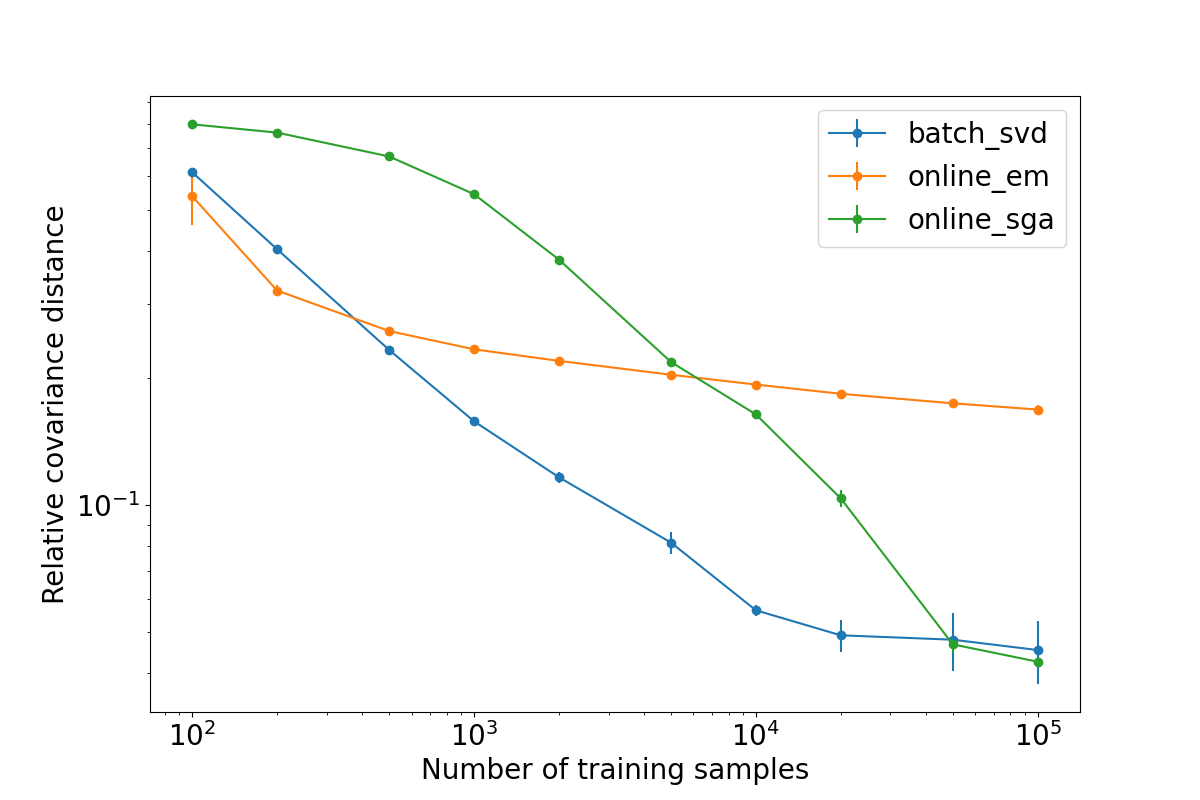
\includegraphics[width=70mm]{plots/online_fa_covar_distance__observation_dim=100__latent_dim=10__spectrum_min=1__spectrum_max=10.png}
		 & 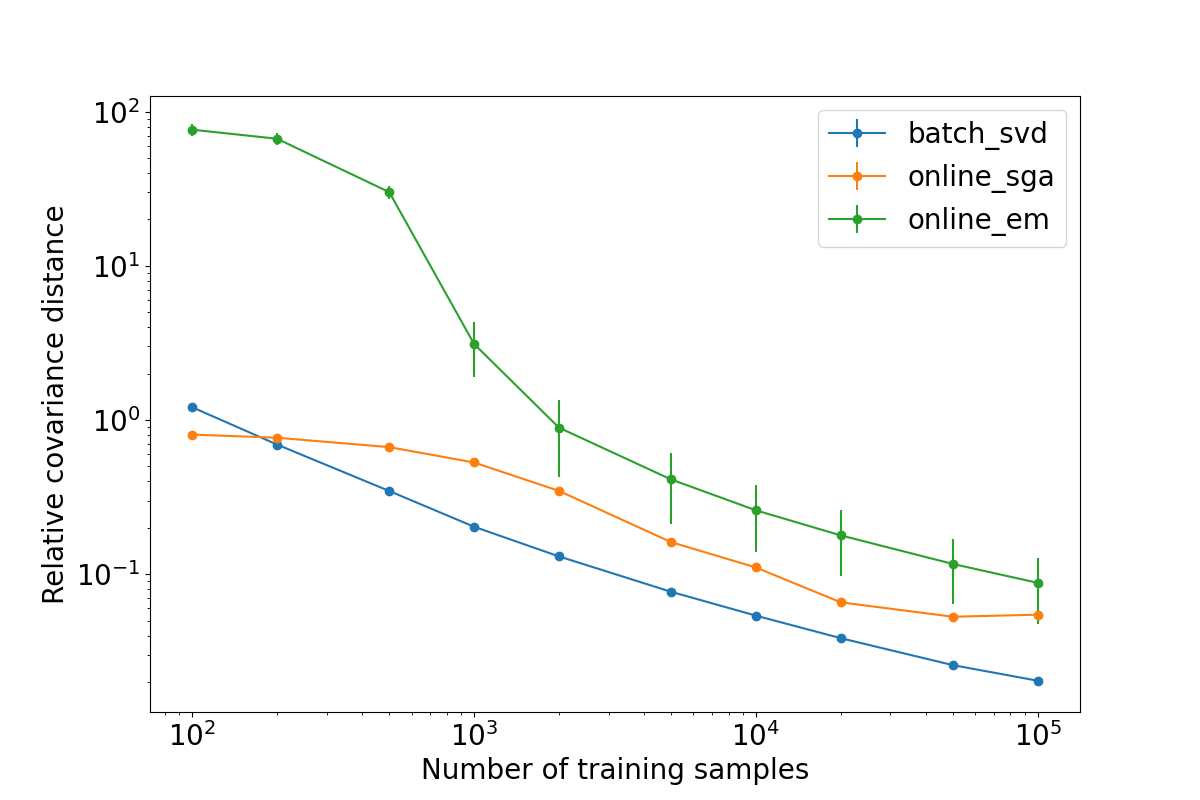
\includegraphics[width=70mm]{plots/online_fa_covar_distance__observation_dim=1000__latent_dim=10__spectrum_min=1__spectrum_max=10.png} \\
		 (a) $D=100$, $K=10$, $\matr{s}^2 \sim \mathcal{U}(1, 10)$ 
		 & (b) $D=1000$, $K=10$, $\matr{s}^2 \sim \mathcal{U}(1, 10)$\\[6pt]
		 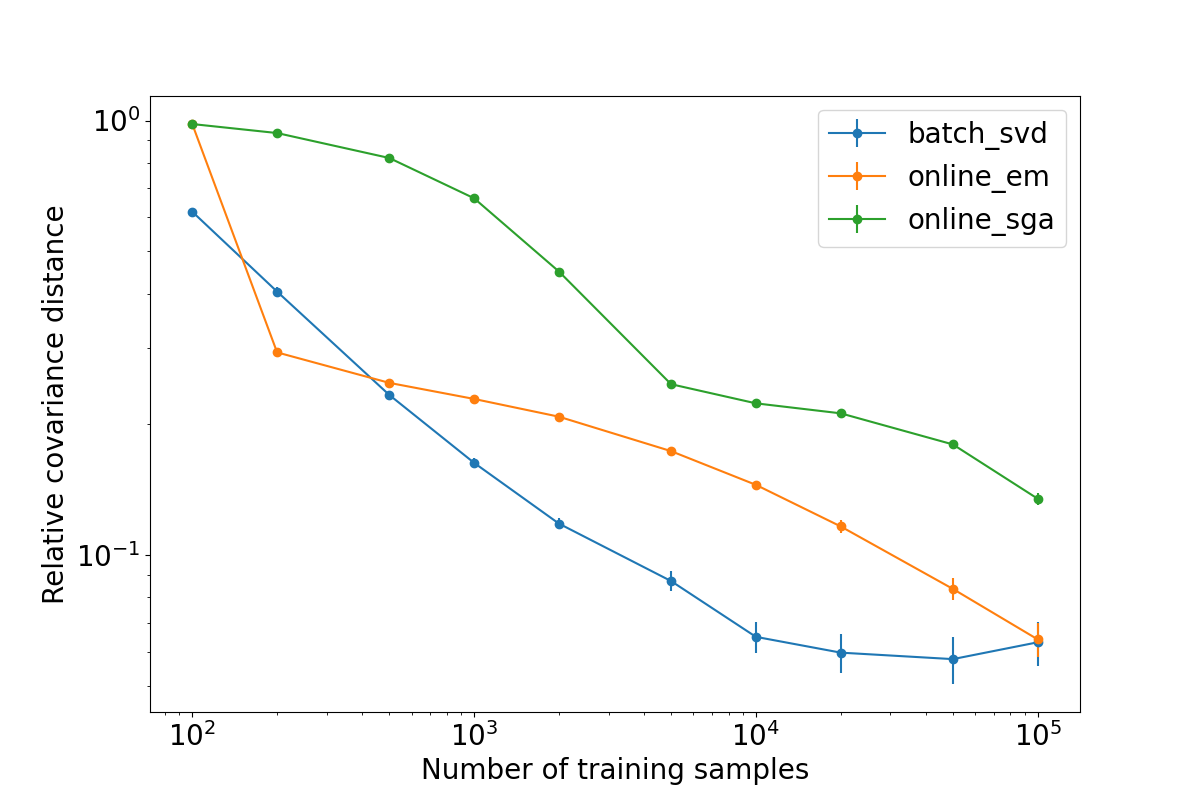
\includegraphics[width=70mm]{plots/online_fa_covar_distance__observation_dim=100__latent_dim=10__spectrum_min=1__spectrum_max=100.png}
		 & 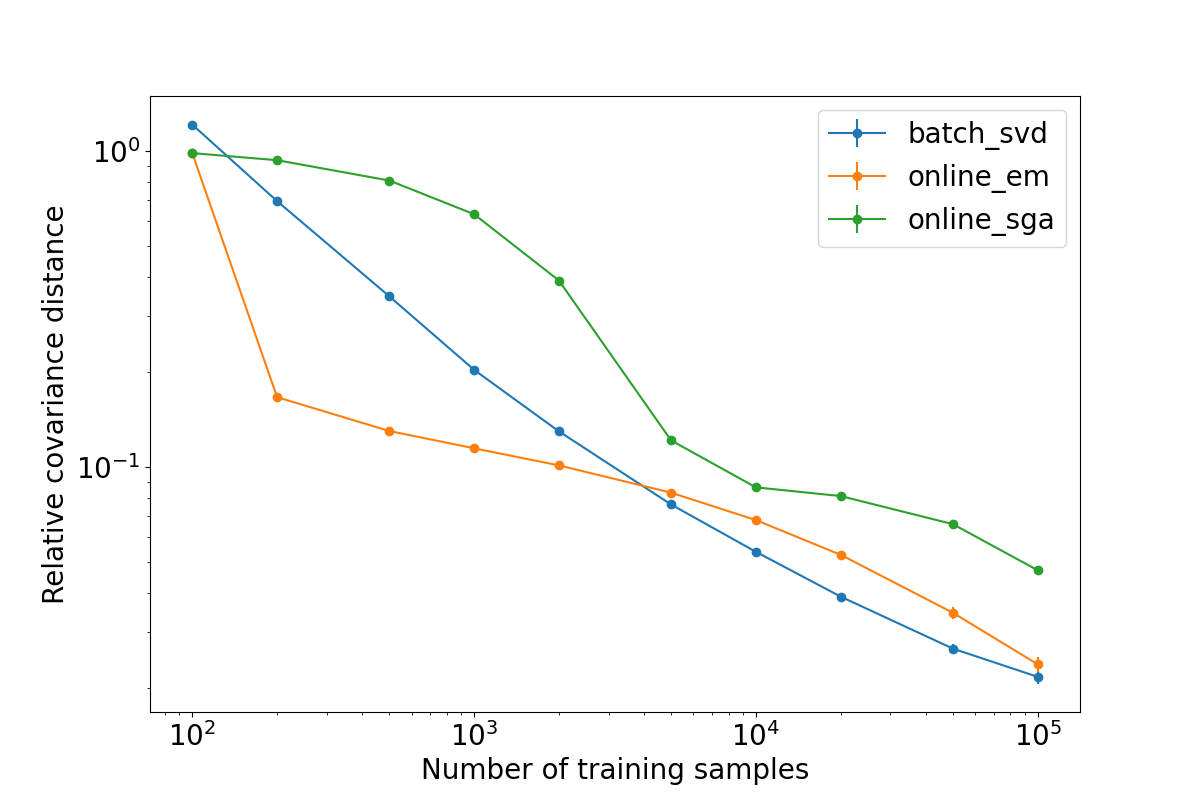
\includegraphics[width=70mm]{plots/online_fa_covar_distance__observation_dim=1000__latent_dim=10__spectrum_min=1__spectrum_max=100.png} \\
		 (c) $D=100$, $K=10$, $\matr{s}^2 \sim \mathcal{U}(1, 100)$ 
		 & (d) $D=1000$, $K=10$, $\matr{s}^2 \sim \mathcal{U}(1, 100)$\\[6pt]
		 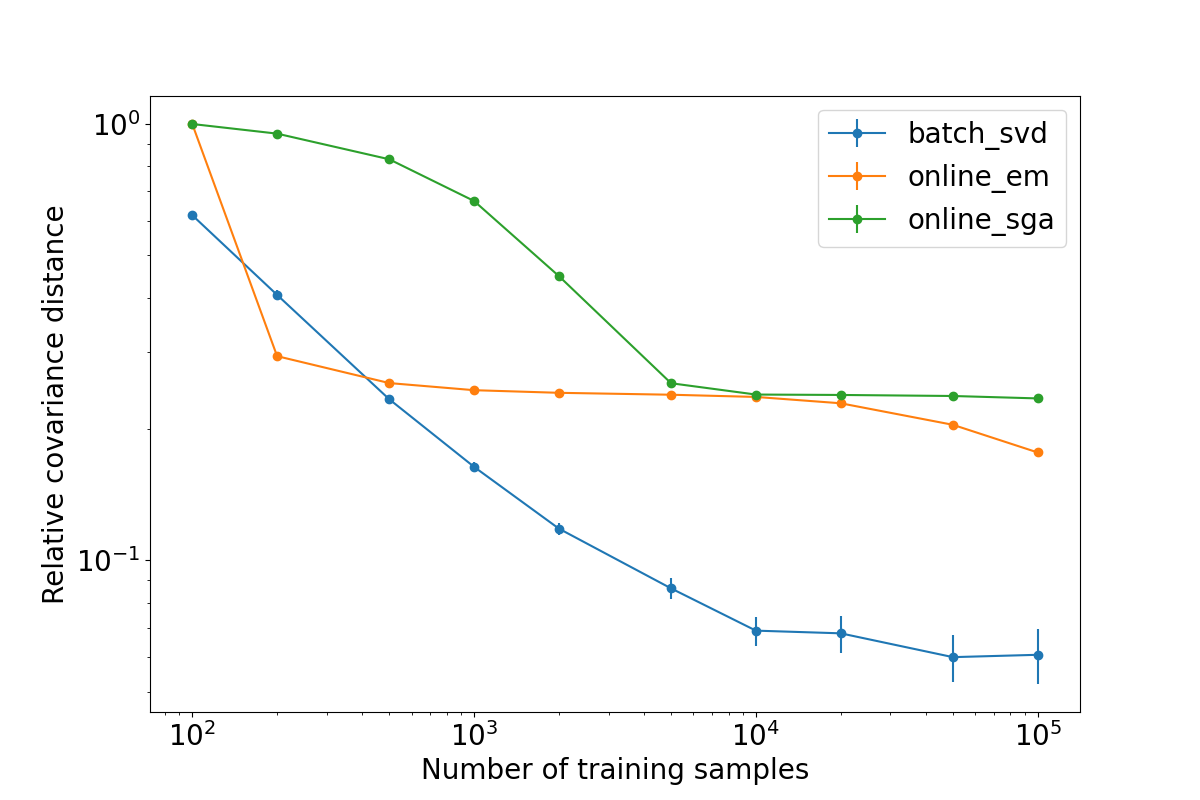
\includegraphics[width=70mm]{plots/online_fa_covar_distance__observation_dim=100__latent_dim=10__spectrum_min=1__spectrum_max=1000.png}
		 & 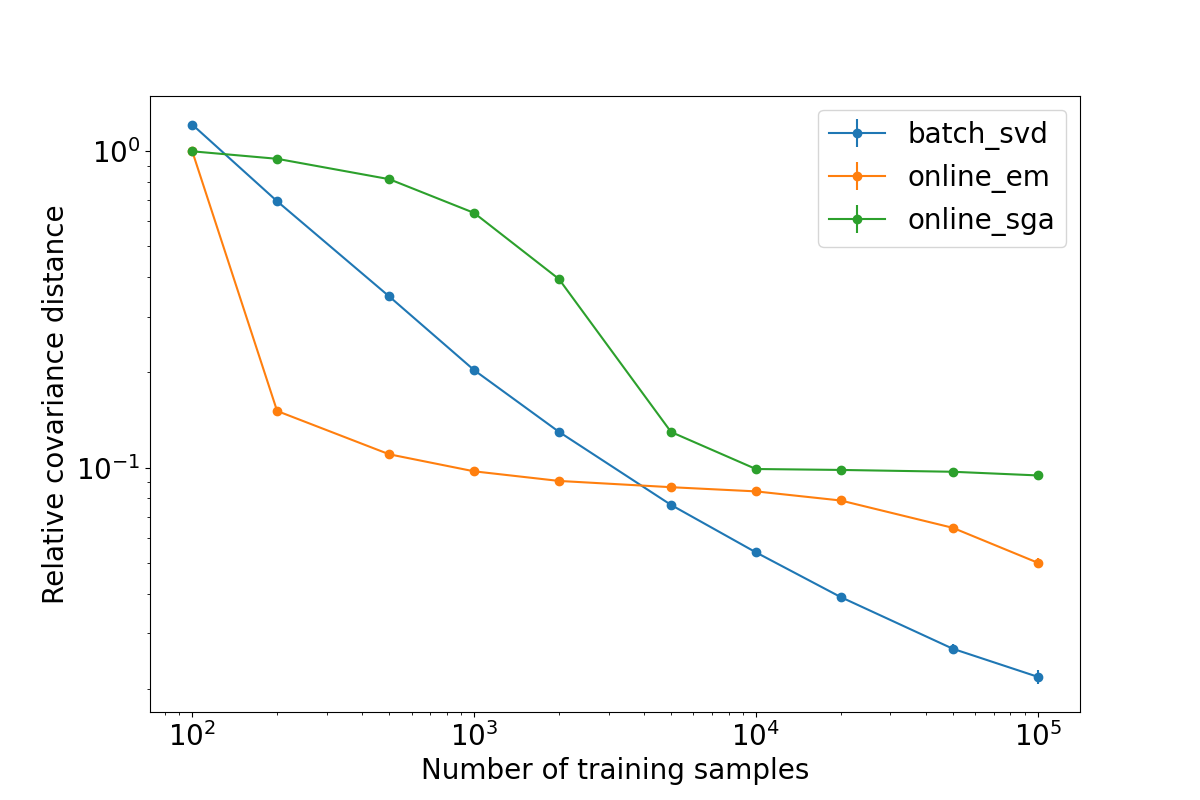
\includegraphics[width=70mm]{plots/online_fa_covar_distance__observation_dim=1000__latent_dim=10__spectrum_min=1__spectrum_max=1000.png} \\
		 (e) $D=100$, $K=10$, $\matr{s}^2 \sim \mathcal{U}(1, 1000)$ 
		 & (f) $D=1000$, $K=10$, $\matr{s}^2 \sim \mathcal{U}(1, 1000)$\\[6pt]
	\end{tabular}
	\caption{The relative distance of the estimated FA covariance matrices from the true covariance matrix as a function of the number of samples used to learn the models. The blue, orange and green lines show, for batch SVD, online EM and online SGA, respectively, the Frobenius norm of the difference between the true covariance matrix and the estimated covariance matrix divided by the Frobenius norm of the true covariance matrix. Each data point shows the mean value over ten trials with different random seeds, and standard error bars are also plotted. The different plots correspond to different combinations of the observation dimension $D$, the latent dimension $K$ and the range of the spectrum $\matr{s}^2$.} 
	\label{fig:fa_covar_distance}
\end{figure}


\begin{figure}[!htbp] 
	\begin{tabular}{cc}
		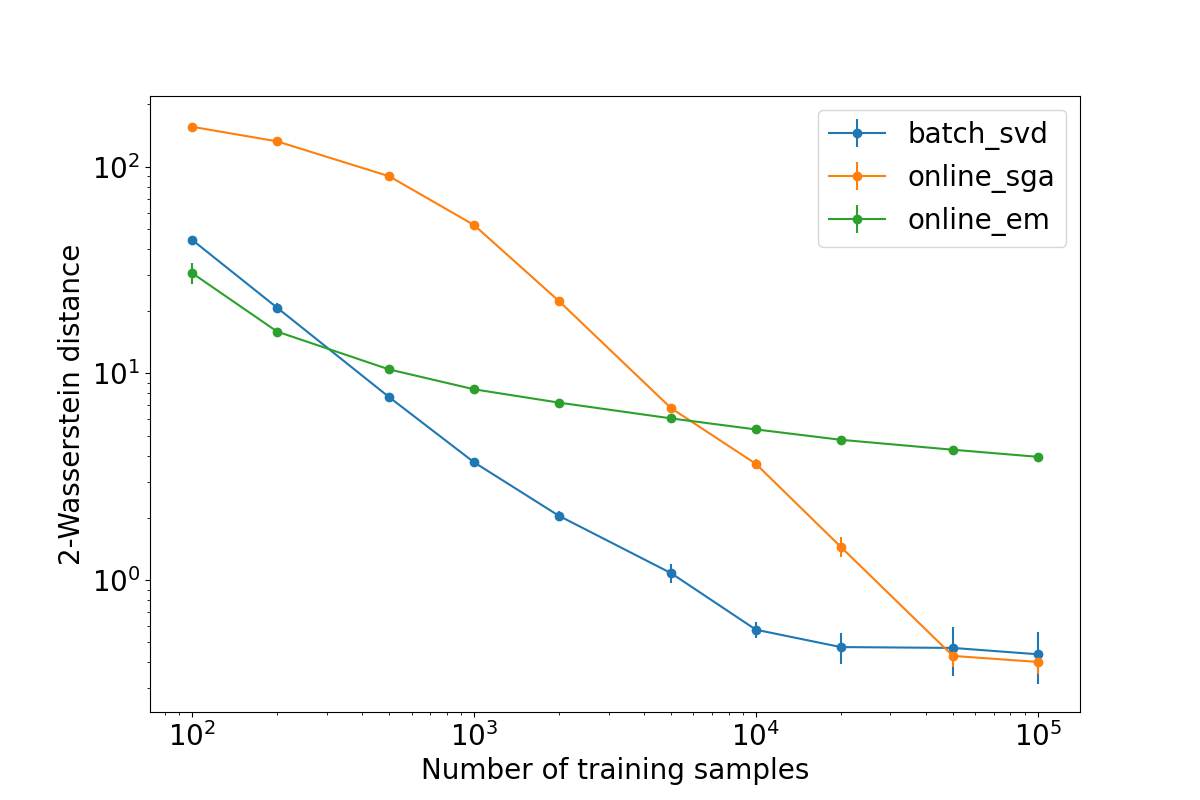
\includegraphics[width=70mm]{plots/online_fa_wasserstein__observation_dim=100__latent_dim=10__spectrum_min=1__spectrum_max=10.png}
		& 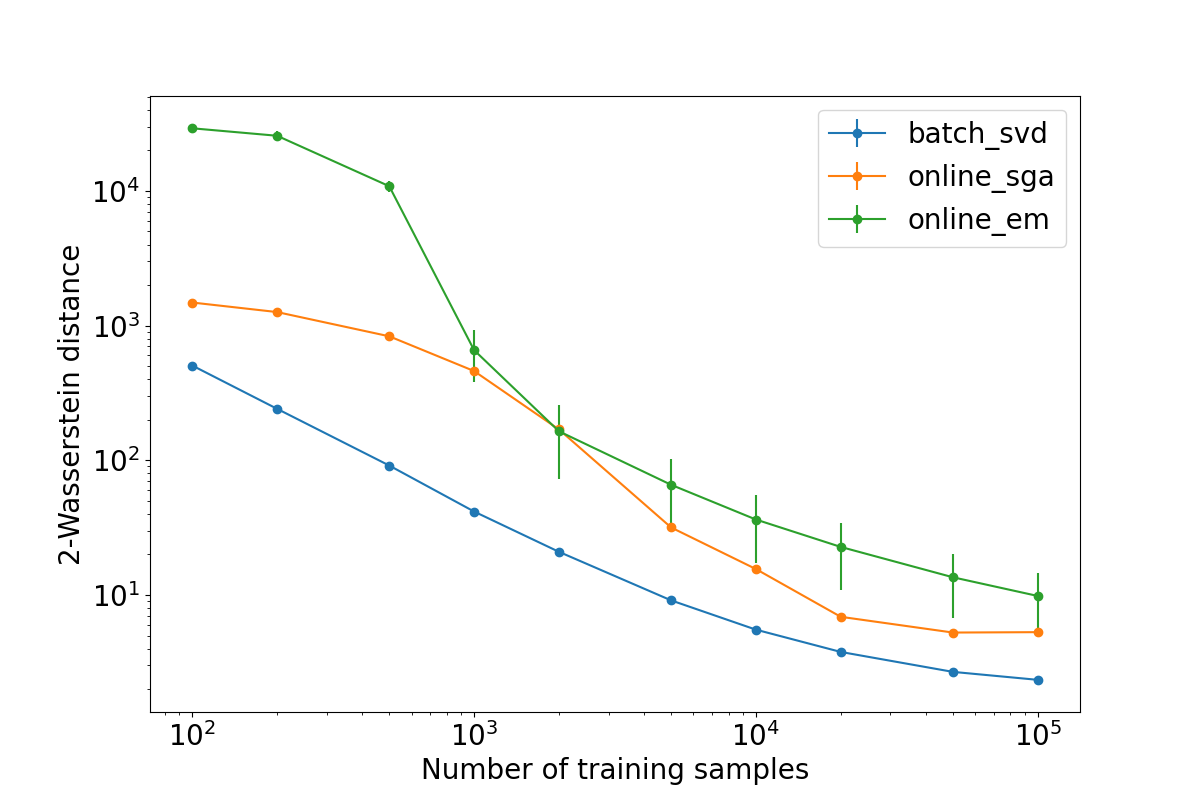
\includegraphics[width=70mm]{plots/online_fa_wasserstein__observation_dim=1000__latent_dim=10__spectrum_min=1__spectrum_max=10.png} \\
		(a) $D=100$, $K=10$, $\matr{s}^2 \sim \mathcal{U}(1, 10)$ 
		 & (b) $D=1000$, $K=10$, $\matr{s}^2 \sim \mathcal{U}(1, 10)$\\[6pt] 
		 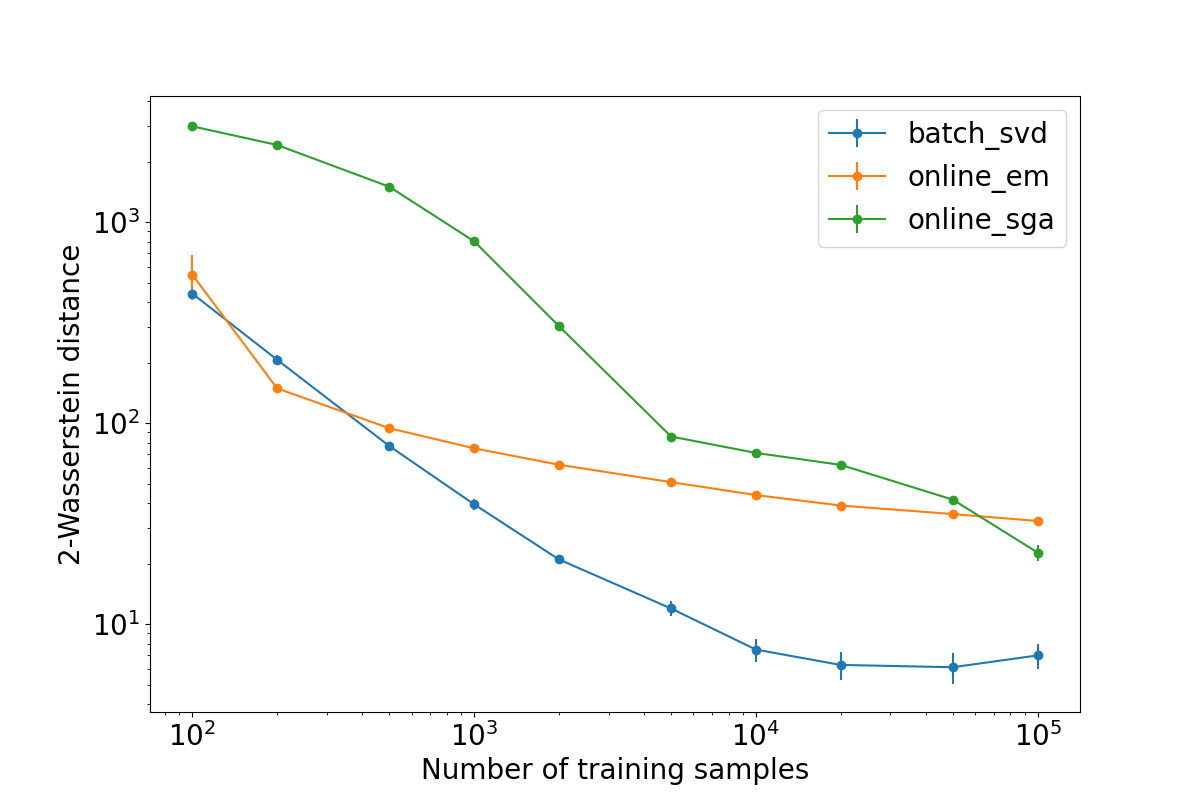
\includegraphics[width=70mm]{plots/online_fa_wasserstein__observation_dim=100__latent_dim=10__spectrum_min=1__spectrum_max=100.png} 
		 & 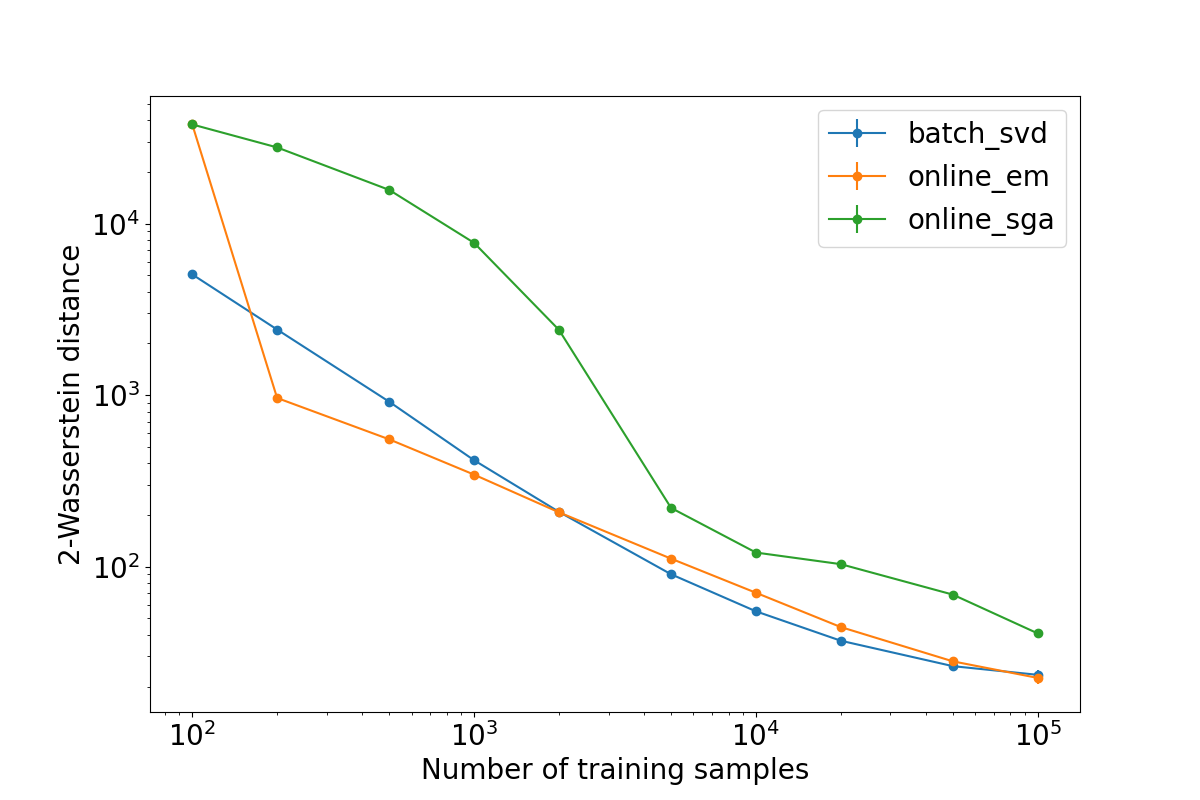
\includegraphics[width=70mm]{plots/online_fa_wasserstein__observation_dim=1000__latent_dim=10__spectrum_min=1__spectrum_max=100.png} \\
		 (c) $D=100$, $K=10$, $\matr{s}^2 \sim \mathcal{U}(1, 100)$ 
		 & (d) $D=1000$, $K=10$, $\matr{s}^2 \sim \mathcal{U}(1, 100)$\\[6pt]
		 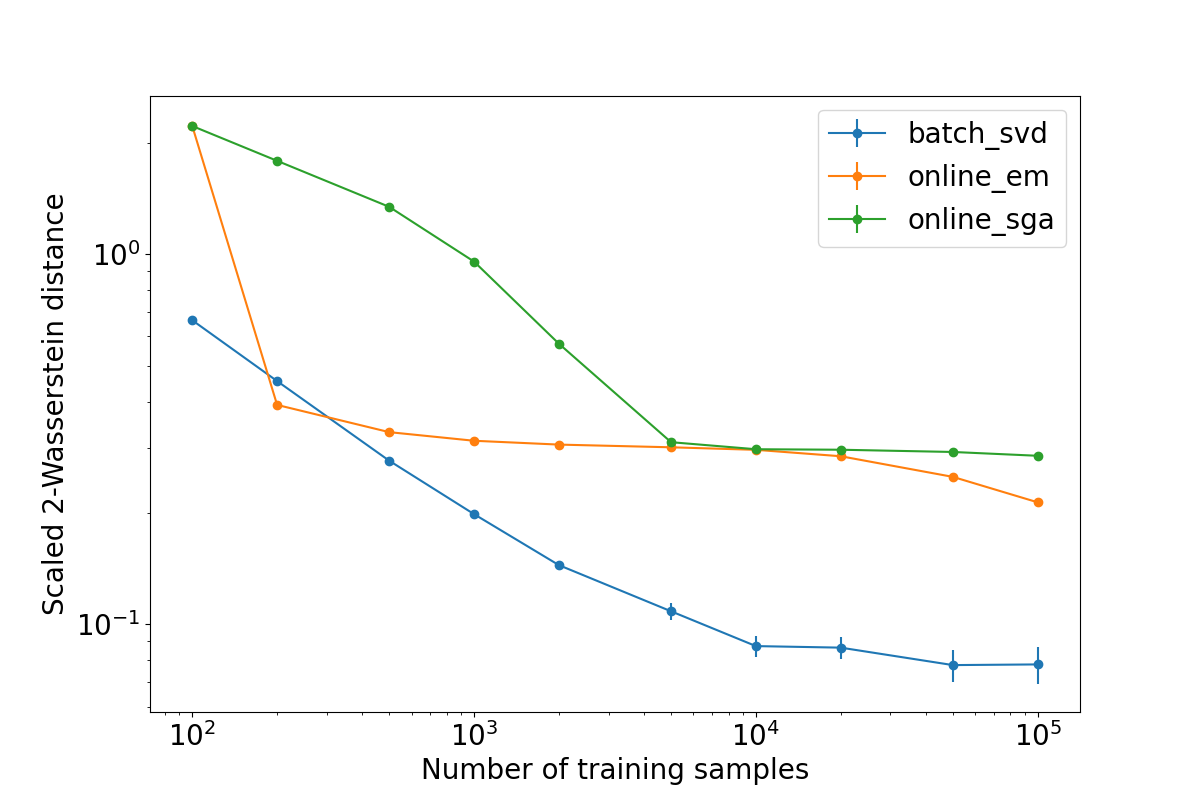
\includegraphics[width=70mm]{plots/online_fa_wasserstein__observation_dim=100__latent_dim=10__spectrum_min=1__spectrum_max=1000.png} 
		 & 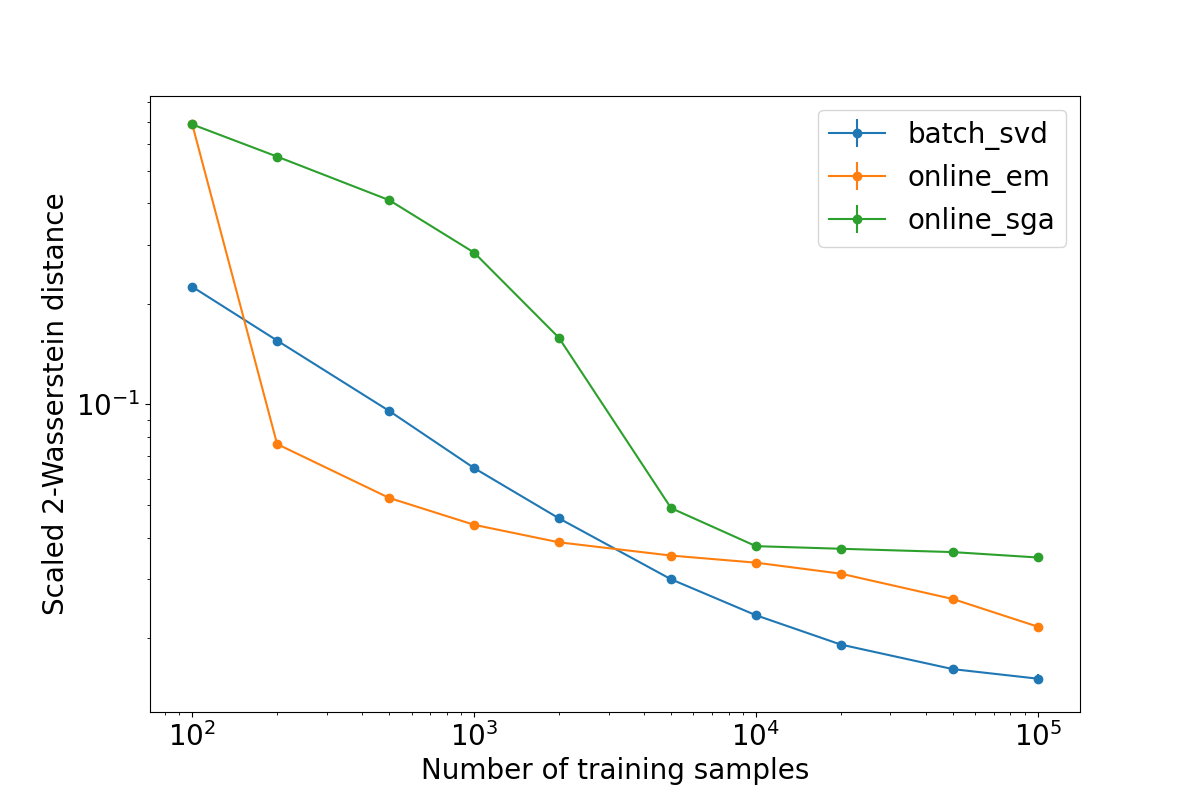
\includegraphics[width=70mm]{plots/online_fa_wasserstein__observation_dim=1000__latent_dim=10__spectrum_min=1__spectrum_max=1000.png} \\
		 (e) $D=100$, $K=10$, $\matr{s}^2 \sim \mathcal{U}(1, 1000)$ 
		 & (f) $D=1000$, $K=10$, $\matr{s}^2 \sim \mathcal{U}(1, 1000)$\\[6pt]
	\end{tabular}
	\caption{The 2-Wasserstein distance between the Gaussian distribution defined by each estimated FA model and the Gaussian distribution defined by the true FA model, divided by the observation dimension. The blue, orange and green lines show the 2-Wasserstein distance corresponding to batch SVD, online EM and online SGA, respectively. Each data point shows the mean value over ten trials with different random seeds, and standard error bars are also plotted. The different plots correspond to different combinations of the observation dimension $D$, the latent dimension $K$ and the range of the spectrum $\matr{s}^2$.}
	\label{fig:fa_wasserstein}
\end{figure}


\chapter{Linear Regression Experiments}\label{ch:linear_regression_experiments}

\section{Posterior Estimation with Synthetic Data}\label{sec:linear_regression_posterior_experiments}

The ability of Algorithms \ref{alg:gradient_fa} and \ref{alg:online_em} to learn the posterior of a neural network's parameter vector hinges on obtaining samples of the parameter vector which are representative of the true posterior. In the SWAG approach, such samples are thought to be obtained from the iterates of the parameter vector which are encountered along the SGD trajectory while training the neural network with a high constant learning rate, following an initial pre-training phase \cite{maddox2019}. In the case of linear regression - which is a neural network with no hidden layers - this assumption can be tested directly, since the true posterior of its parameter vector can be computed in closed form. Recall, however, that the posterior distribution in Equation (\ref{eqn:linear_regression_posterior}) refers to specific values of $\alpha$ and $\beta$. The parameter $\beta$ is $\frac{1}{\sigma^2}$, where $\sigma$ is the standard deviation of the outputs $y_n$ in Equation (\ref{eqn:linear_regression_pdf}). The precision $\alpha$ is a hyperparameter which controls the width of the prior $p(\theta)$. In Equation (\ref{eqn:linear_regression_log_posterior}), the log-posterior of $\theta$ was written as 
\begin{equation}
	\log p(\theta | \mathcal{D}) 
	= -\frac{\beta}{2} \sum_{n=1}^N \big(y_n - \theta^\intercal \matr{x}_n \big)^2 
	-\frac{\alpha}{2} \theta^\intercal \theta 
	+ \text{constant}.
\end{equation}
Hence, the maximum \emph{a posteriori} (MAP) estimate of $\theta$ is that which maximises
\begin{equation}
	-\frac{\beta}{2} \sum_{n=1}^N \big(y_n - \theta^\intercal \matr{x}_n \big)^2 
	-\frac{\alpha}{2} \theta^\intercal \theta.
\end{equation}
Since $\beta > 0$, it is equivalent to minimise this expression scaled by $-\frac{2}{\beta}$, that is,
\begin{equation}
	\sum_{n=1}^N \big(y_n - \theta^\intercal \matr{x}_n \big)^2 
	+ \frac{\alpha}{\beta} \theta^\intercal \theta.
\end{equation}
This objective function is analogous to the L2-regularised training loss often used in non-Bayesian linear regression \cite{barber2007}, which is 
\begin{equation}\label{eqn:regularised_linear_regression}
	\sum_{n=1}^N \big(y_n - \theta^\intercal \matr{x}_n \big)^2 
	+ \lambda \theta^\intercal \theta 
\end{equation}
for some $\lambda > 0$. Setting $\lambda = \frac{\alpha}{\beta}$, the optimal $\theta$ found by L2-regularised linear regression is the same as the MAP estimate of $\theta$ in Bayesian linear regression with prior $p(\theta) = \mathcal{N}\big(\matr{0}, \alpha^{-1} \matr{I} \big)$. This means that, given data $\mathcal{D}$ and a particular value of $\alpha$, the SGD iterates sampled while minimising Equation (\ref{eqn:regularised_linear_regression}) with $\lambda = \frac{\alpha}{\beta}$ should in theory by representative of the true posterior $p(\theta | \mathcal{D})$. Also, for the same data $\mathcal{D}$ and hyperparameters $\alpha$ and $\beta$, the VI approach in Algorithm \ref{alg:vi_fa} should be able to approximate $p(\theta | \mathcal{D})$ directly. The purpose of the experiments in this section is to test these hypotheses. 
 
\subsection{Methodology}

Synthetic data was generated for these experiments as follows. First, 1000 inputs $\matr{x} \in \R^2$ were sampled from a multivariate zero mean Gaussian distribution with covariance matrix
\begin{equation}
	\begin{bmatrix}
		1 & 0.5 \\
		0.5 & 1
	\end{bmatrix}.
\end{equation}
Next, the parameter vector $\theta \in \R^2$ was sampled from $\mathcal{N}\big(\matr{0}, \alpha^{-1} \matr{I} \big)$ with $\alpha = 0.01$. Then the outputs $y \in \R$ were generated according to Equation (\ref{eqn:linear_regression}) with $\beta = 0.1$. Using this data, the true posterior in Equation (\ref{eqn:linear_regression_posterior}) was evaluated. 

For the purpose of obtaining samples from the posterior, the linear regression model was pre-trained for 500 epochs of SGD with a learning rate of 0.001 and a batch size of 100. Then, starting from the pre-trained model, a further 100 epochs of SGD were executed, during which the parameter vector sampled after each mini-batch gradient update was collected. During the collection period, the batch size was again set to 100 but different values of the learning rate were tested, namely 0.1 and 0.01. As for regularisation, as well as the theoretically motivated value of $\lambda = \frac{\alpha}{\beta} = 0.1$, a value of $\lambda = 0.001$ was also tested. Since there were $\frac{1000}{100} = 10$ batch updates per epoch, a total of 1000 parameter vectors were collected over the final 100 epochs. The empirical mean and covariance of these samples was then computed and compared to the ground truth. 

For the VI experiments, Algorithm \ref{alg:vi_fa} was executed with the same synthetic data and precision $\alpha$. In this case, the training process ran for 5000 epochs with a batch size of $M=100$ and a Monte Carlo average size of $L=10$.  The learning rates $\eta_\matr{c}$,  $\eta_\matr{F}$ and $\eta_\beta$ were set to 0.01, 0.0001 and 0.01, respectively. The reason for using a smaller learning rate for $\matr{F}$ is that its contribution to the full covariance matrix is $\matr{F}\matr{F}^\intercal$. Two different latent dimensions were tested for the approximate FA posterior, namely $K=1$ and $K=2$. When computing the log-likelihood term involved in the gradient calculations, the variance of the outputs $y$ was set to the true value, $\sigma^2 = \frac{1}{\beta} = 10$. Finally, to improve numerical stability, any gradients with Frobenius norm greater than 10 were rescaled to have norm of exactly 10. 

All experiments were repeated ten times. In each trial a different random seed was used for generating the data, the true parameter vector and the initial parameters of the linear regression model. 

\subsection{Results and Discussion}

The results of the posterior sampling experiments are shown in Table \ref{table:linear_regression_samples}. It is apparent from the third column that the empirical mean of the sampled parameter vectors does not match the true posterior mean when the theoretically motivated value of $\lambda = 0.1$ is used. However, if the regularisation strength is reduced to $\lambda = 0.001$, the distance between the means is much smaller. Unfortunately, the distance between the covariance matrices of the two distributions is relatively large for all combinations of the hyperparameters, as can be seen in the fourth column. The best result is achieved when using a learning rate of 0.1 with $\lambda = 0.1$, but even then the average relative distance is 0.62. 

\begin{table}[h!]
	\begin{center}
		\begin{tabular}{|| p{0.12\linewidth} p{0.1\linewidth} p{0.21\linewidth} p{0.21\linewidth} p{0.21\linewidth} ||} 
 			\hline
 			Learning Rate & $\lambda$ & Relative Distance from Mean & Relative Distance from Covariance & Scaled Wasserstein Distance \\ [0.5ex] 
 			\hline\hline
 			0.1 	&  0.1 	& $0.0666 \pm 0.0078$	& $0.6200 \pm 0.0750$	& $0.4946 \pm 0.1013$ \\ 
			\hline
 			0.1 	& 0.001	& $0.0006 \pm 0.0001$	& $0.8065 \pm 0.0101$ 	& $0.0439 \pm 0.0012$  \\
			\hline
			0.01	& 0.1 	& $0.0620 \pm 0.0070$	& $1.7110 \pm 0.6187$ 	& $0.4641 \pm 0.0937$ \\ 
			\hline
 			0.01	& 0.001 	& $0.0010 \pm 0.0002$ 	& $0.9870 \pm 0.0042$ 	& $0.0739 \pm 0.0010$  \\ [1ex] 
			\hline
		\end{tabular}
		\caption{Distances between the true posterior distribution of the parameter vector of a linear regression model and the empirical distribution of the parameter vectors sampled along the SGD trajectory while training the model. Relative distances between the true and empirical means and covariances are shown. Each relative distance is the Frobenius norm of the difference between the true parameter and the empirical parameter divided by the Frobenius norm of the true parameter. Also shown is the 2-Wasserstein distance between the true posterior Gaussian distribution and the empirical Gaussian distribution, divided by the dimension of the distribution. Each distance is the mean value over ten trials with different random seeds, and standard errors are also given.}
		\label{table:linear_regression_samples}
	\end{center}
\end{table}

Figure \ref{fig:linear_regression_pdfs} shows, for each combination of the hyperparameters, the sampled parameter vectors for one of the ten trials in each posterior sampling experiment. These are plotted on top of the contours of the pdf of the true posterior distribution. Note that in each case the pre-trained parameter vector is very close to the true posterior mean. When $\lambda = 0.1$, SGD moves away from the pre-trained solution to a different region of the parameter space (subplots (a) and (c)). When $\lambda = 0.001$, SGD bounces around the pre-trained solution and the empirical mean of the parameter vectors, $\theta_{\text{SWA}}$, is right on the true posterior mean. However, when the learning rate is 0.1 the empirical covariance is in the wrong direction (subplot (b)), and when the learning rate is 0.01 the empirical covariance is far too narrow (subplot (d)).

\begin{figure}[!htbp] 
	\begin{tabular}{cc}
		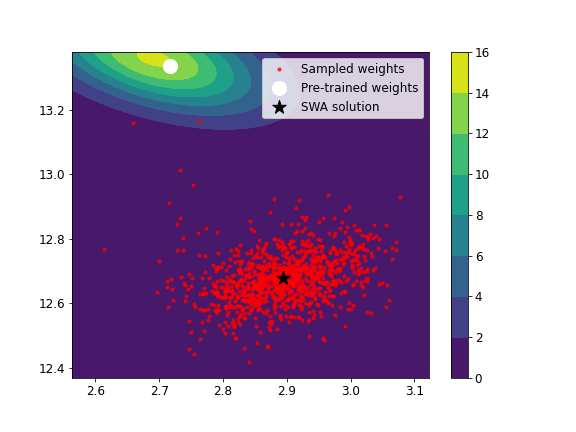
\includegraphics[width=70mm]{plots/linear_model_weight_iterates__lr=0.1__lambda=0.1.png}
		& 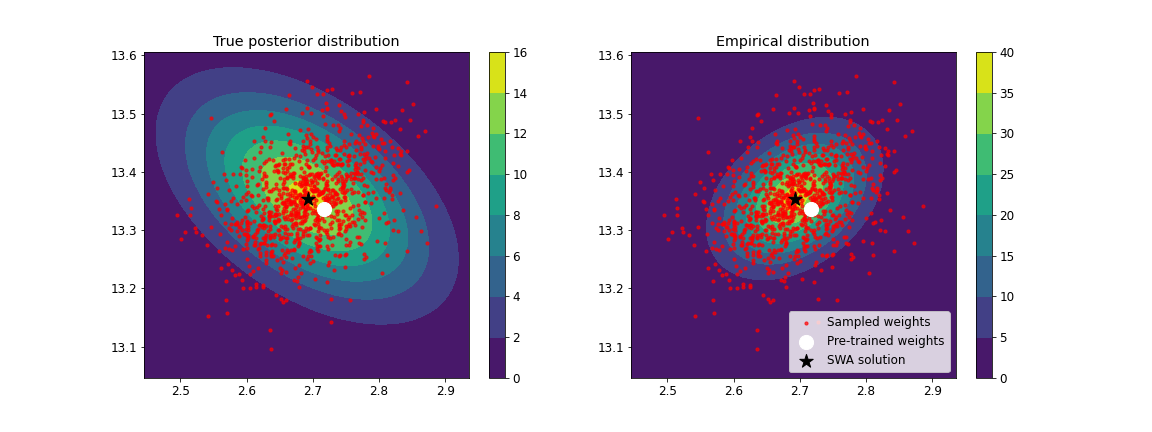
\includegraphics[width=70mm]{plots/linear_model_weight_iterates__lr=0.1__lambda=0.001.png} \\
		(a) Learning rate of 0.1 and $\lambda = 0.1$
		 & (b) Learning rate of 0.1 and $\lambda = 0.001$ \\[6pt] 
		 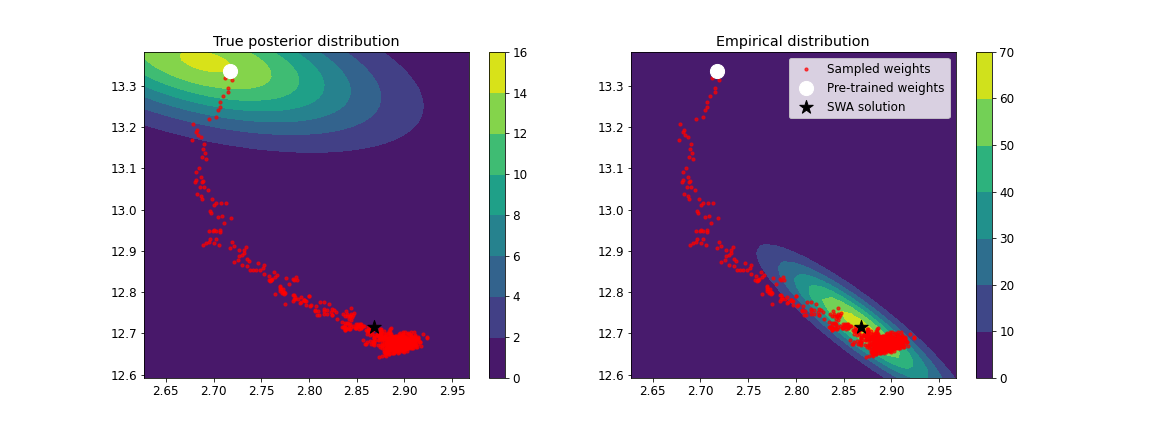
\includegraphics[width=70mm]{plots/linear_model_weight_iterates__lr=0.01__lambda=0.1.png}
		 & 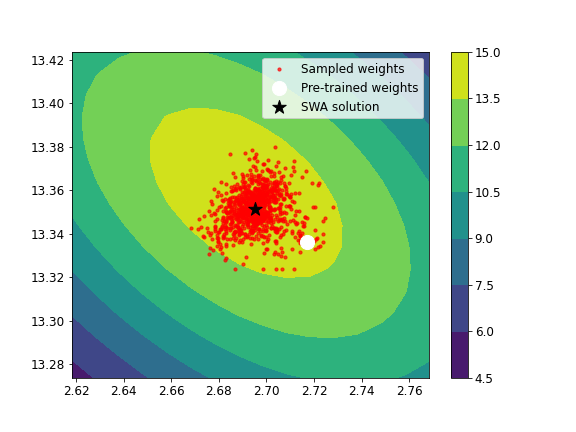
\includegraphics[width=70mm]{plots/linear_model_weight_iterates__lr=0.01__lambda=0.001.png} \\
		 (c) Learning rate of 0.01 and $\lambda = 0.1$
		 & (d) Learning rate of 0.01 and $\lambda = 0.001$ \\[6pt]
	\end{tabular}
	\caption{Parameter vectors sampled while training a linear regression model via SGD, for different combinations of learning rate and regularisation strength. These are shown as red dots, plotted on top of the contours of the pdf of the true posterior distribution. In each plot, the white dot denotes the pre-trained parameter vector and the black star is the empirical mean of the red dots.}
	\label{fig:linear_regression_pdfs}
\end{figure}

These results suggest that, in general, SGD does not sample parameter vectors from the true posterior distribution. This is a very simple example of a linear model in two dimensions. Even when tuning the learning rate and regularisation strength, it is not possible to obtain samples which are representative of the true posterior. For certain values of $\lambda$ (but not the theoretically motivated one), the mean solution $\theta_{\text{SWA}}$ is a good approximation of the true posterior mean, but the same cannot be said for the empirical covariance. The most that can be expected of the online FA algorithms is that they fit the sampled parameter vectors well. Therefore, given the data observed in Figure \ref{fig:linear_regression_pdfs}, it would be unreasonable to expect them to learn the true posterior distribution. In the case of a high-dimensional multi-layer neural network, approximating the true posterior would be even more unlikely. Since the ground truth cannot be compute in closed form, hyperparameter tuning would be far more difficult. Therefore, contrary to what is claimed in \cite{maddox2019}, this suggest that SWAG does not actually do approximate Bayesian inference in general.

It was also observed in \cite{mandt2017} that the empirical covariance of the linear regression SGD iterates does not match the true posterior covariance. As such, the authors proposed a different technique for posterior sampling called \emph{finite window iterate averaging}. Instead of using the individual parameter vectors sampled after each mini-batch update of SGD, this algorithm averages the parameter vectors in fixed-length disjoint windows. These average parameter vectors are then considered samples from the posterior. Figure \ref{fig:linear_regression_average_iterates} shows examples of such samples for the same learning rate and regularisation strength as that in Figure \ref{fig:linear_regression_pdfs} (b). The theoretical work in \cite{mandt2017} suggests that the window size should be set to the number of training examples divided by the batch size, so that all training examples are use to generate a single posterior sample. In these experiments this value is $1000 / 100 = 10$. However, this setting does not produce samples which are representative of the true posterior, as observed in Figure \ref{fig:linear_regression_average_iterates} (a). Better samples can be obtained by setting the batch size to 10 and the window size to 50, as shown in Figure \ref{fig:linear_regression_average_iterates} (b). Unfortunately, this result is not theoretically motivated and was only obtained after significant tuning of both the batch size and window size. In the case of non-linear neural networks for which the true posterior is not known, this would not be possible. Therefore, this algorithm does not seem to be a viable option in practice. 

\begin{figure}[!htbp] 
	\begin{tabular}{cc}
		 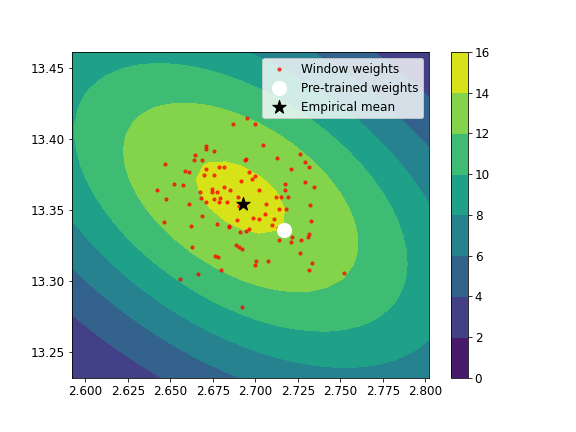
\includegraphics[width=70mm]{plots/linear_model_average_weight_iterates__lr=0.1__lambda=0.001__batch_size=100__window_size=10.png}
		 & 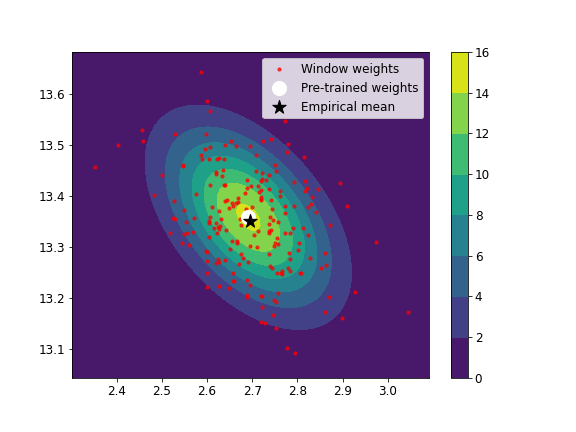
\includegraphics[width=70mm]{plots/linear_model_average_weight_iterates__lr=0.1__lambda=0.001__batch_size=10__window_size=50.png} \\
		 (a) Batch size of 100, window size of 10
		 & (b) Batch size of 10, window size of 50 \\[6pt]
	\end{tabular}
	\caption{Samples constructed via finite window iterate averaging for different combinations of batch size and window size. Each red dot is the mean of a set of linear regression parameter vectors sampled during consecutive mini-batch updates of SGD, with a learning rate of 0.1 and the regularisation strength set to 0.001. The contours show the pdf of the true posterior distribution. The white dot denotes the pre-trained parameter vector and the black star is the empirical mean of the red dots.}
	\label{fig:linear_regression_average_iterates}
\end{figure}

Moving on to VI, the results of applying Algorithm \ref{alg:vi_fa} to the data are shown in Table \ref{table:linear_regression_vi_posterior}. Compared to using the SGD iterates, the more direct VI approach does a much better job of approximating the true covariance matrix. For the FA model with a single latent dimension, the average distance of the estimated covariance from the ground truth is 0.0983, which is much lower than the best result of 0.6200 from Table \ref{table:linear_regression_samples}. The much improved approximation of the covariance can also be observed in Figure \ref{fig:linear_regression_vi_posterior} for one of the ten VI trials. In this example, both the diagonal and off-diagonal entries of the covariance matrices of the two FA models are very similar to the ground truth. Moreover, in these experiments the FA model with a single latent dimension achieved better results than the FA with two latent dimensions. This is encouraging, since applying this algorithm to estimate the posterior of a deep neural network is only feasible if the latent dimension can be set to a value much less than the number of learnable parameters in the model. 

\begin{table}[h!]
	\begin{center}
		\begin{tabular}{|| p{0.21\linewidth} p{0.21\linewidth} p{0.21\linewidth} p{0.21\linewidth} ||} 
 			\hline
 			Latent Dimension of FA Model & Relative Distance from Mean & Relative Distance from Covariance & Scaled Wasserstein Distance \\ [0.5ex] 
 			\hline\hline
			1 	& $0.0031 \pm 0.0005$ 	& $0.0983 \pm 0.0129$ 	& $0.0194 \pm 0.0023$ \\ [1ex] 
			\hline
 			2 	& $0.0040 \pm 0.0008$ 	& $ 0.1053 \pm 0.0199$ 	& $0.0242 \pm 0.0030$ \\ [1ex] 
			\hline
		\end{tabular}
		\caption{Distances between the true posterior distribution of the parameter vector of a linear regression model and the approximate FA posterior estimated using VIFA. Relative distances between the true and approximate means and covariances are shown. Each relative distance is the Frobenius norm of the difference between the true parameter and the approximate parameter divided by the Frobenius norm of the true parameter. Also shown is the 2-Wasserstein distance between the true posterior Gaussian distribution and the approximate Gaussian distribution, divided by the dimension of the distribution. Each distance is the mean value over ten trials with different random seeds, and standard errors are also given.}
		\label{table:linear_regression_vi_posterior}
	\end{center}
\end{table}

\begin{figure}[!htbp] 
	\begin{tabular}{cc}
		 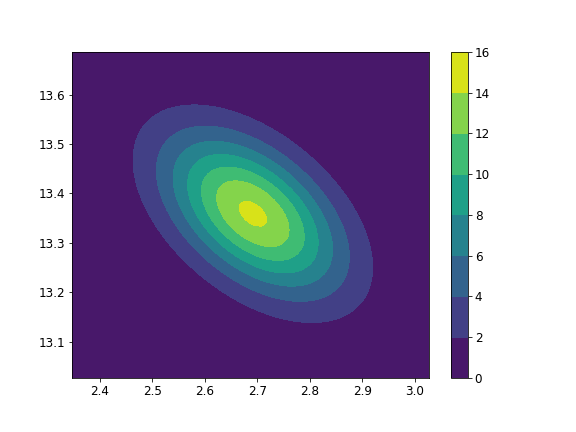
\includegraphics[width=70mm]{plots/linear_model_true_posterior__alpha=0.01__beta=0.1.png}
		 & 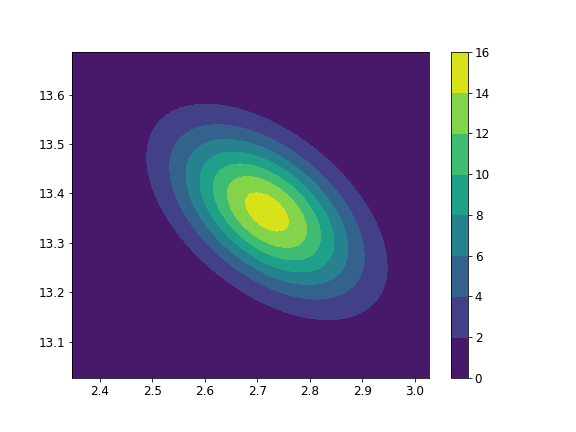
\includegraphics[width=70mm]{plots/linear_model_vi_posterior__alpha=0.01__beta=0.1__latent_dim=1.png} \\
		 (a) Ground truth
		 & (b) VIFA: latent dim = 1 \\
		 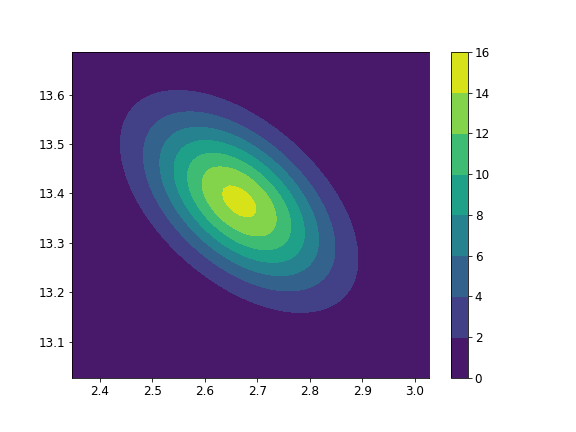
\includegraphics[width=70mm]{plots/linear_model_vi_posterior__alpha=0.01__beta=0.1__latent_dim=2.png} \\
		 (c) VIFA: latent dim = 2 \\[6pt]
	\end{tabular}
	\caption{The true posterior pdf of a linear regression model with two learnable parameters, plus the pdfs of two FA models fit to the same data using VIFA. Both approximations are very similar to the ground truth, including the FA model with only a single latent dimension.}
	\label{fig:linear_regression_vi_posterior}
\end{figure}


\section{Posterior Estimation with UCI Datasets}

Given the positive results achieved by VIFA in the experiments using synthetic data, the purpose of these experiments is to test how well VIFA is able to approximate the posterior of linear regression models fit to real datasets with more dimensions. Methods based on stochastic weight averaging are excluded from these experiments, given that they were unable to obtain representative samples from simple synthetic posteriors with only two dimensions. 

\subsection{Methodology}

For these experiments, four regression datasets from the UCI Machine Learning Repository \cite{dua2019} were used. Namely, the Energy Efficiency\footnote{https://archive.ics.uci.edu/ml/datasets/energy+efficiency}, Boston Housing\footnote{https://archive.ics.uci.edu/ml/machine-learning-databases/housing}, Concrete Compressive Strength\footnote{https://archive.ics.uci.edu/ml/datasets/concrete+compressive+strength} and Yacht Hydrodynamics\footnote{http://archive.ics.uci.edu/ml/datasets/yacht+hydrodynamics} datasets. More details about these datasets are given in Table \ref{table:uci_datasets}. Note that the original Energy Efficiency dataset has two target variables, heating load and cooling load, but in these experiments only the heating load was used. 

\begin{table}[h!]
	\begin{center}
		\begin{tabular}{||c c c ||} 
			\hline
 			Dataset & No. of Instances & No. of Input Variables \\ [0.5ex] 
			\hline\hline
			Energy Efficiency 				& 768 	& 8 \\
 			\hline
 			Boston Housing 				& 506 	& 13 \\ 
 			\hline
 			Concrete Compressive Strength 	& 1030 	& 8 \\
 			\hline
 			Yacht Hydrodynamics 			& 308 	& 6 \\ [1ex] 
 			\hline
		\end{tabular}
		\caption{UCI regression datasets used in experiments.}
		\label{table:uci_datasets}
	\end{center}
\end{table}

Each dataset was split into validation and test sets of equal size. The VIFA hyperparameters were tuned on the validation set and then the algorithm was evaluated once on the test set. The final VIFA hyperparameter values for each dataset are shown in Table \ref{table:vifa_uci_hyperparameters}. Note that the latent dimension $K$ was not tuned. Instead it was set to roughly half the dimension of each dataset. Also, a single learning rate $\eta$ was used to optimise all parameters. That is, $\eta_\matr{c} = \eta_\matr{F} = \eta_\beta = \eta$. Again, to improve numerical stability, any gradients with Frobenius norm greater than 10 were rescaled to have norm of exactly 10. The hyperparameters $\alpha$ and $\beta$ correspond to the precision of the prior and the precision of the noise distribution of the target variable, respectively. These were defined formally in Section \ref{sec:bayesian_lr}.

\begin{table}[h!]
	\begin{center}
		\begin{tabular}{||c c c c c c c c||} 
			\hline
 			Dataset & $K$ & Epochs & $M$ & $L$ & $\eta$ & $\alpha$ & $\beta$ \\ [0.5ex] 
			\hline\hline
			Energy Efficiency 				& 4 & 20,000 & 100 & 10 	& 0.01 	& 0.0539 & 0.1082 \\ 
 			\hline
			Boston Housing 				& 6 & 20,000 & 100 & 10 	& 0.001 	& 0.2523 & 0.0462 \\
 			\hline
 			Concrete Compressive Strength	& 4 & 20,000 & 100 & 10 	& 0.01 	& 0.0278 & 0.0086 \\
 			\hline
 			Yacht Hydrodynamics 			& 3 & 30,000 & 100 & 10 	& 0.01 	& 0.0371 & 0.0139 \\ [1ex] 
 			\hline
		\end{tabular}
		\caption{VIFA hyperparameters for linear regression posterior estimation experiments with UCI datasets.}
		\label{table:vifa_uci_hyperparameters}
	\end{center}
\end{table}

The \texttt{BayesianRidge} estimator from the scikit-learn library \cite{pedregosa2012} was used to compute the ground truth posterior. This algorithm automatically selects $\alpha$ and $\beta$ via the Bayesian method described in \cite{mackay1992}. These ground truth values, which are given in Table \ref{table:vifa_uci_hyperparameters}, were also used when running VIFA. Note, the reason that $\beta$ is not mentioned explicitly in Algorithm \ref{alg:vi_fa} is that no reference was made to the specific form of the likelihood distribution. However, in these linear regression experiments the likelihood is Gaussian and its precision is set to $\beta$. Finally, before running the algorithms, each input variable was re-scaled to have zero mean and unit standard deviation.  

\subsection{Results and Discussion}

Figure \ref{fig:posterior_energy_efficiency} shows a qualitative comparison of the true posterior of a linear regression model fit to the Energy Efficiency dataset and the approximate posterior learned by VIFA. Figures \ref{fig:posterior_boston_housing}, \ref{fig:posterior_concrete_strength} and \ref{fig:posterior_yacht_hydrodynamics} show the same comparison for the Boston Housing, Concrete Compressive Strength and Yacht Hydrodynamics datasets, respectively. Quantitative results are also given in Table \ref{table:linear_regression_vi_posterior_uci}.

TODO: add discussion once we add test results

\begin{figure}[!htbp] 
	\begin{tabular}{c}
		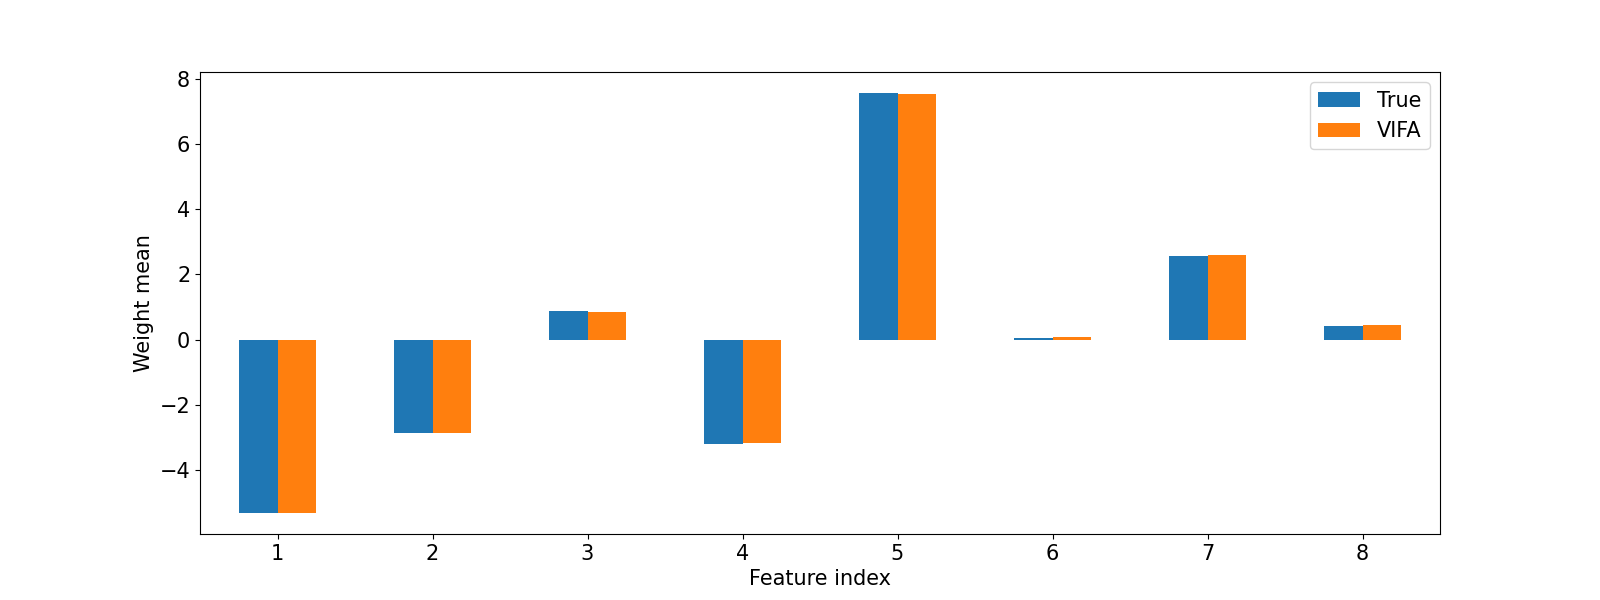
\includegraphics[width=140mm]{plots/energy_efficiency_posterior_mean.png} \\
		(a) Comparison of true and estimated posterior means \\[6pt] 
		 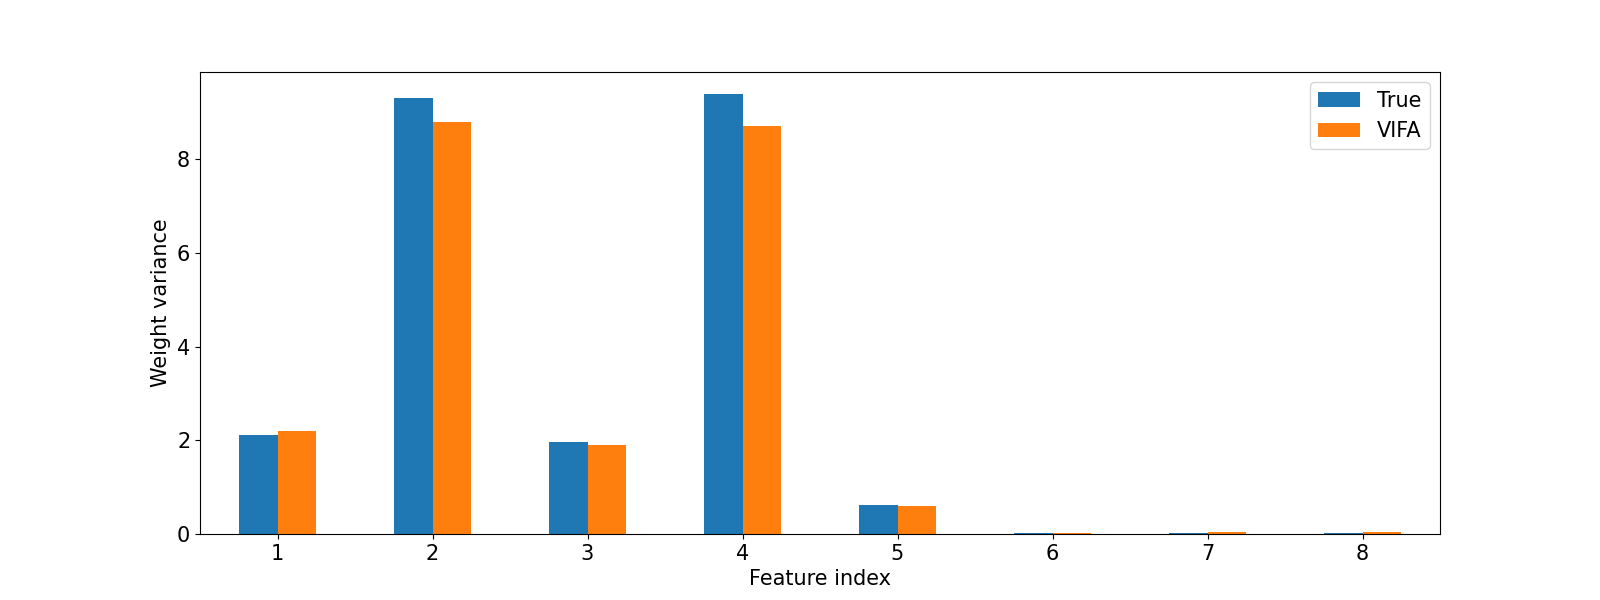
\includegraphics[width=140mm]{plots/energy_efficiency_posterior_variance.png} \\
		(b) Comparison of true and estimated posterior variances \\[6pt] 
		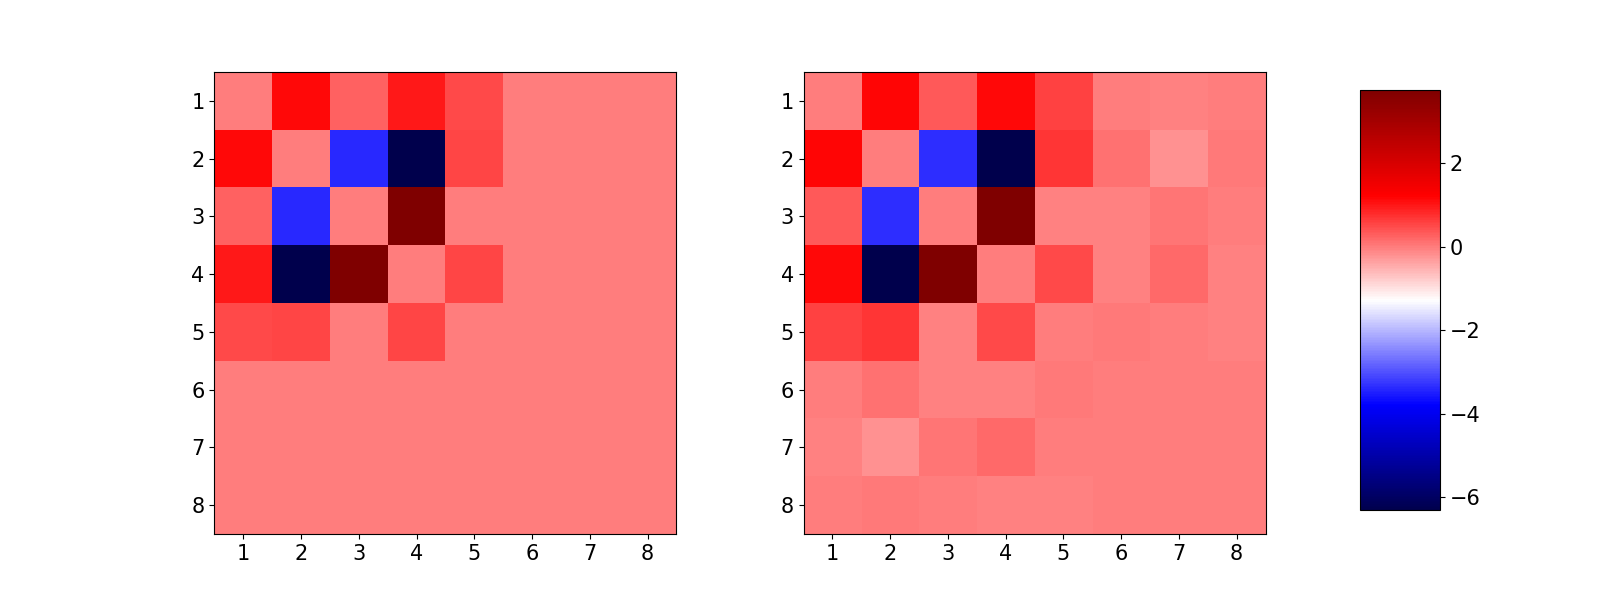
\includegraphics[width=140mm]{plots/energy_efficiency_posterior_covariance.png} \\
		(c) Comparison of true and estimated posterior covariances \\[6pt] 
	\end{tabular}
	\caption{Comparison of the ground truth posterior of a linear regression model fit to the Energy Efficiency dataset, and the approximate posterior learned by VIFA. Variances and covariance are plotted separately due to the difference in their magnitude. In plot (c), the diagonal entries of the covariance matrices have been set to zero.}
	\label{fig:posterior_energy_efficiency}
\end{figure}

\begin{figure}[!htbp] 
	\begin{tabular}{c}
		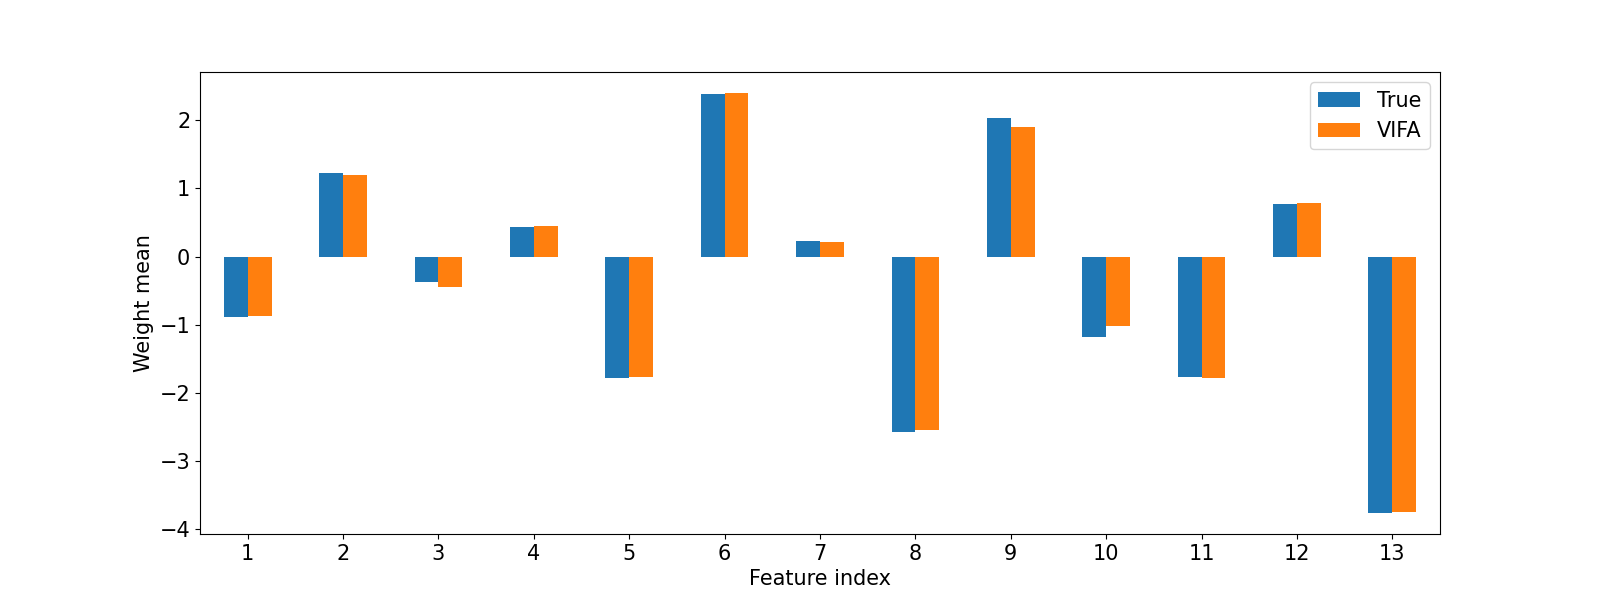
\includegraphics[width=140mm]{plots/boston_housing_posterior_mean.png} \\
		(a) Comparison of true and estimated posterior means \\[6pt] 
		 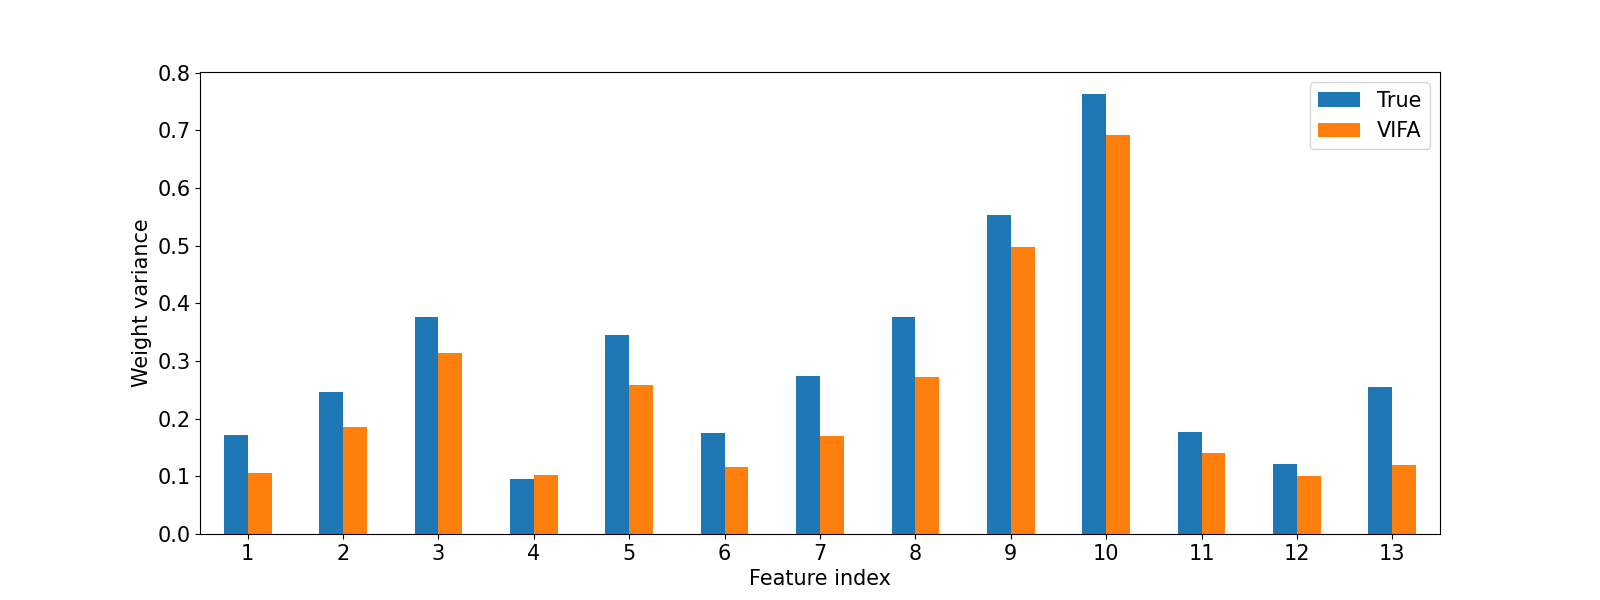
\includegraphics[width=140mm]{plots/boston_housing_posterior_variance.png} \\
		(b) Comparison of true and estimated posterior variances \\[6pt] 
		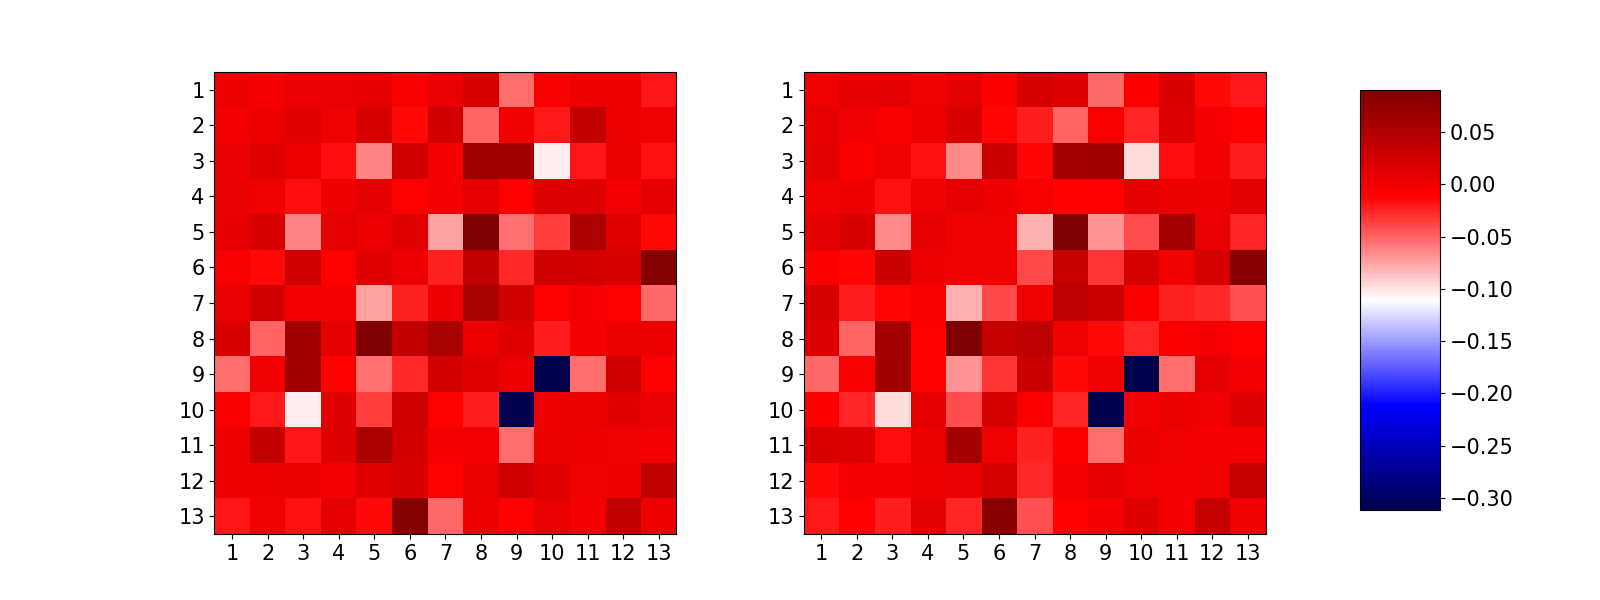
\includegraphics[width=140mm]{plots/boston_housing_posterior_covariance.png} \\
		(c) Comparison of true and estimated posterior covariances \\[6pt] 
	\end{tabular}
	\caption{Comparison of the ground truth posterior of a linear regression model fit to the Boston Housing dataset, and the approximate posterior learned by VIFA. Variances and covariance are plotted separately due to the difference in their magnitude. In plot (c), the diagonal entries of the covariance matrices have been set to zero.}
	\label{fig:posterior_boston_housing}
\end{figure}

\begin{figure}[!htbp] 
	\begin{tabular}{c}
		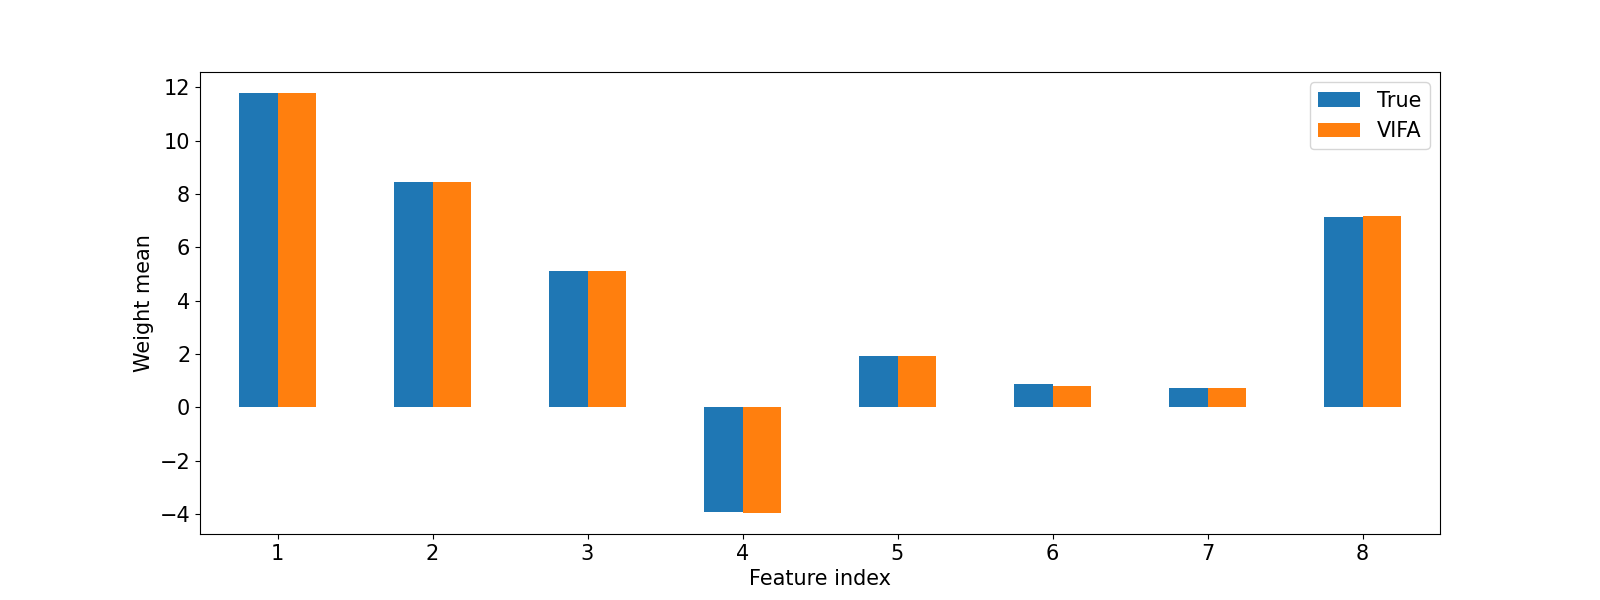
\includegraphics[width=140mm]{plots/concrete_strength_posterior_mean.png} \\
		(a) Comparison of true and estimated posterior means \\[6pt] 
		 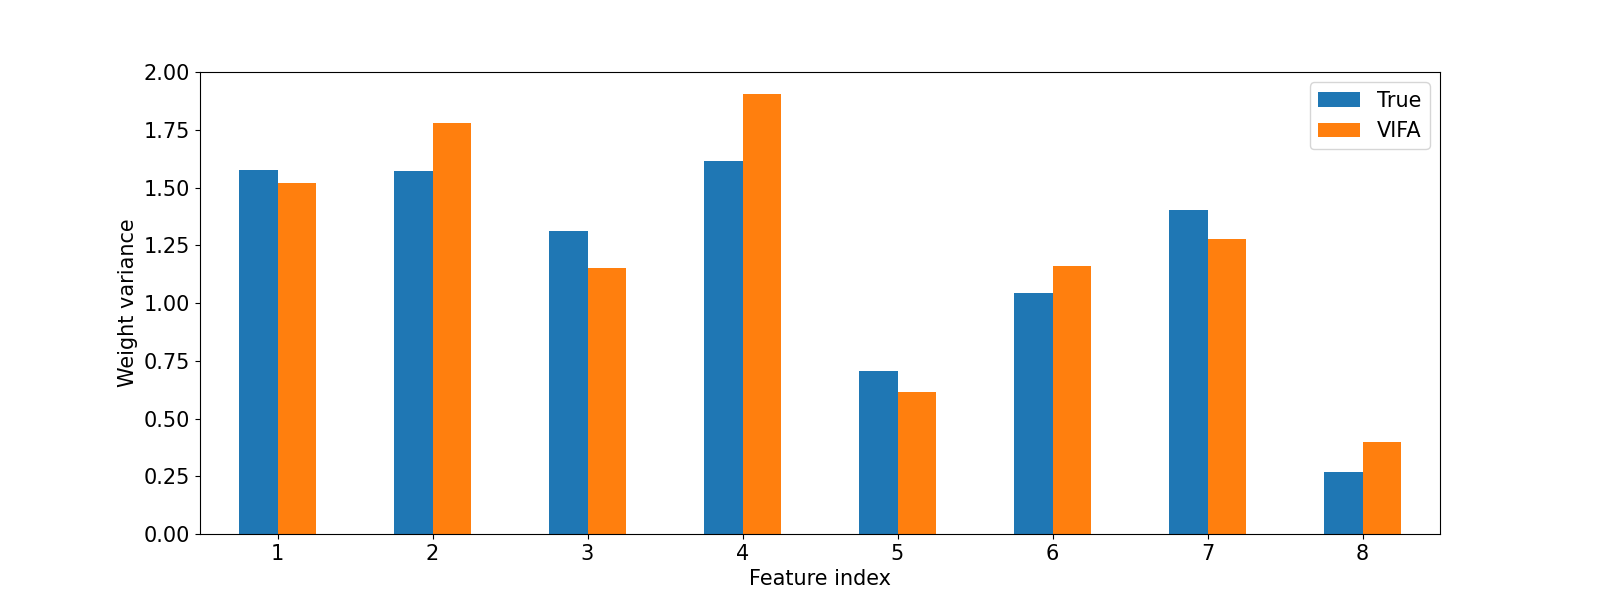
\includegraphics[width=140mm]{plots/concrete_strength_posterior_variance.png} \\
		(b) Comparison of true and estimated posterior variances \\[6pt] 
		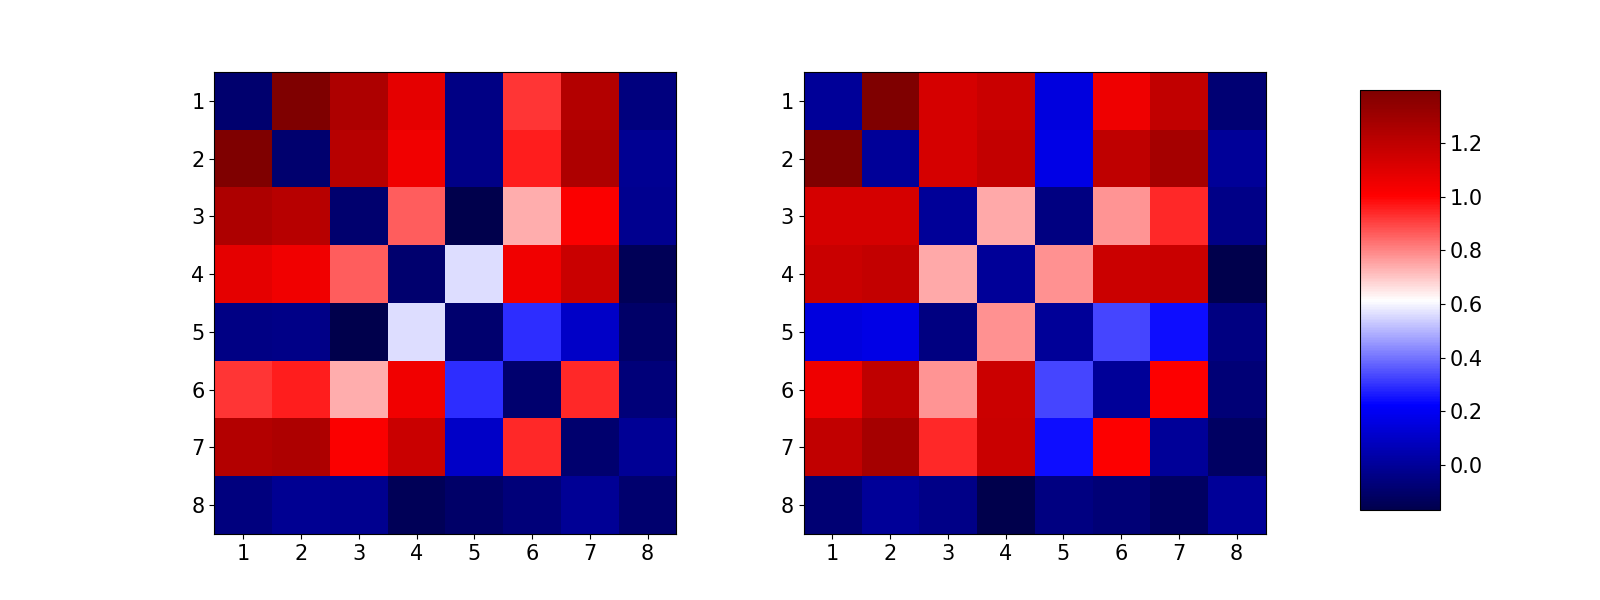
\includegraphics[width=140mm]{plots/concrete_strength_posterior_covariance.png} \\
		(c) Comparison of true and estimated posterior covariances \\[6pt] 
	\end{tabular}
	\caption{Comparison of the ground truth posterior of a linear regression model fit to the Concrete Compressive Strength dataset, and the approximate posterior learned by VIFA. Variances and covariance are plotted separately due to the difference in their magnitude. In plot (c), the diagonal entries of the covariance matrices have been set to zero.}
	\label{fig:posterior_concrete_strength}
\end{figure} 

\begin{figure}[!htbp] 
	\begin{tabular}{c}
		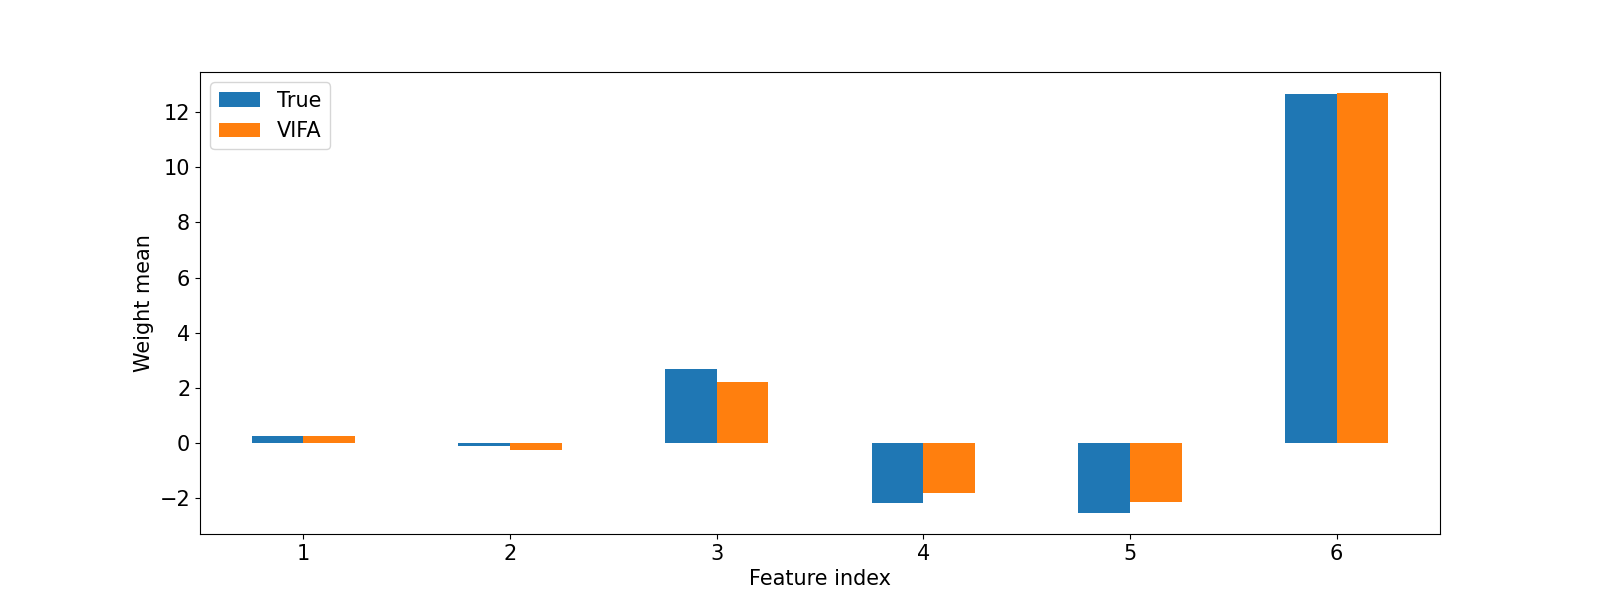
\includegraphics[width=140mm]{plots/yacht_hydrodynamics_posterior_mean.png} \\
		(a) Comparison of true and estimated posterior means \\[6pt] 
		 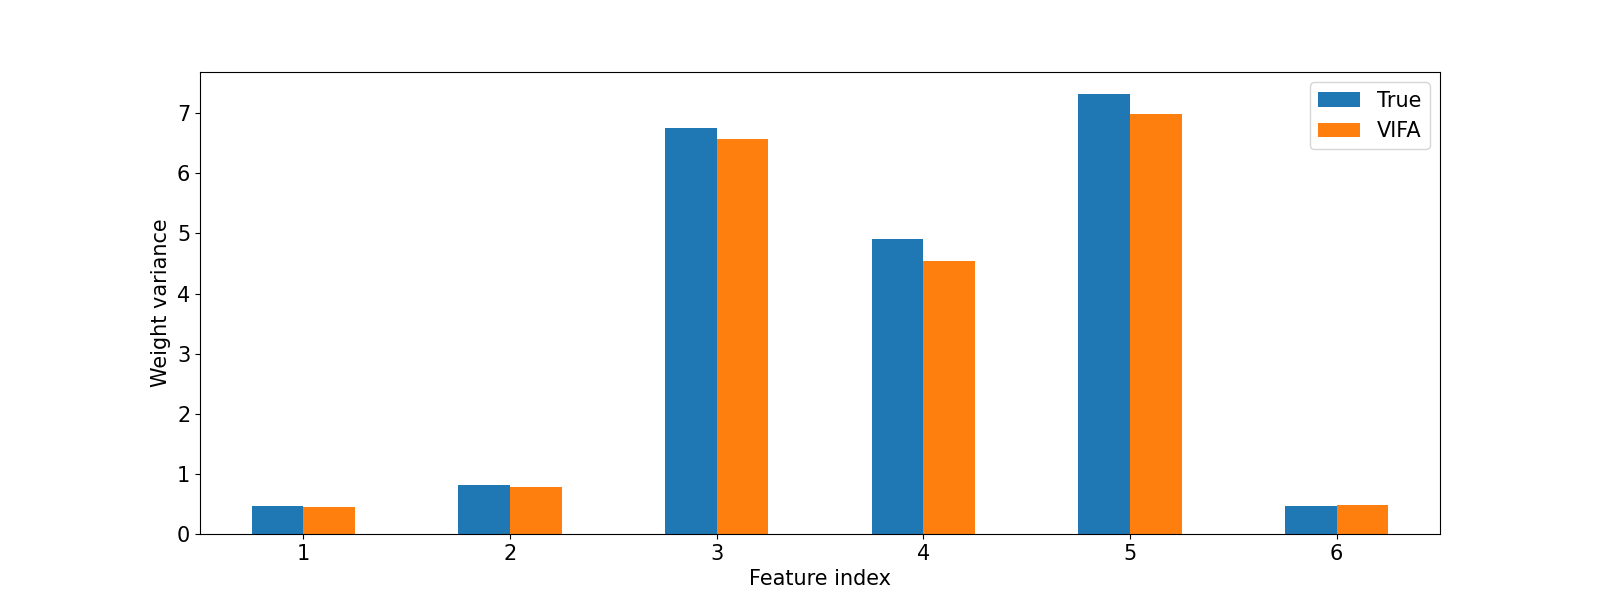
\includegraphics[width=140mm]{plots/yacht_hydrodynamics_posterior_variance.png} \\
		(b) Comparison of true and estimated posterior variances \\[6pt] 
		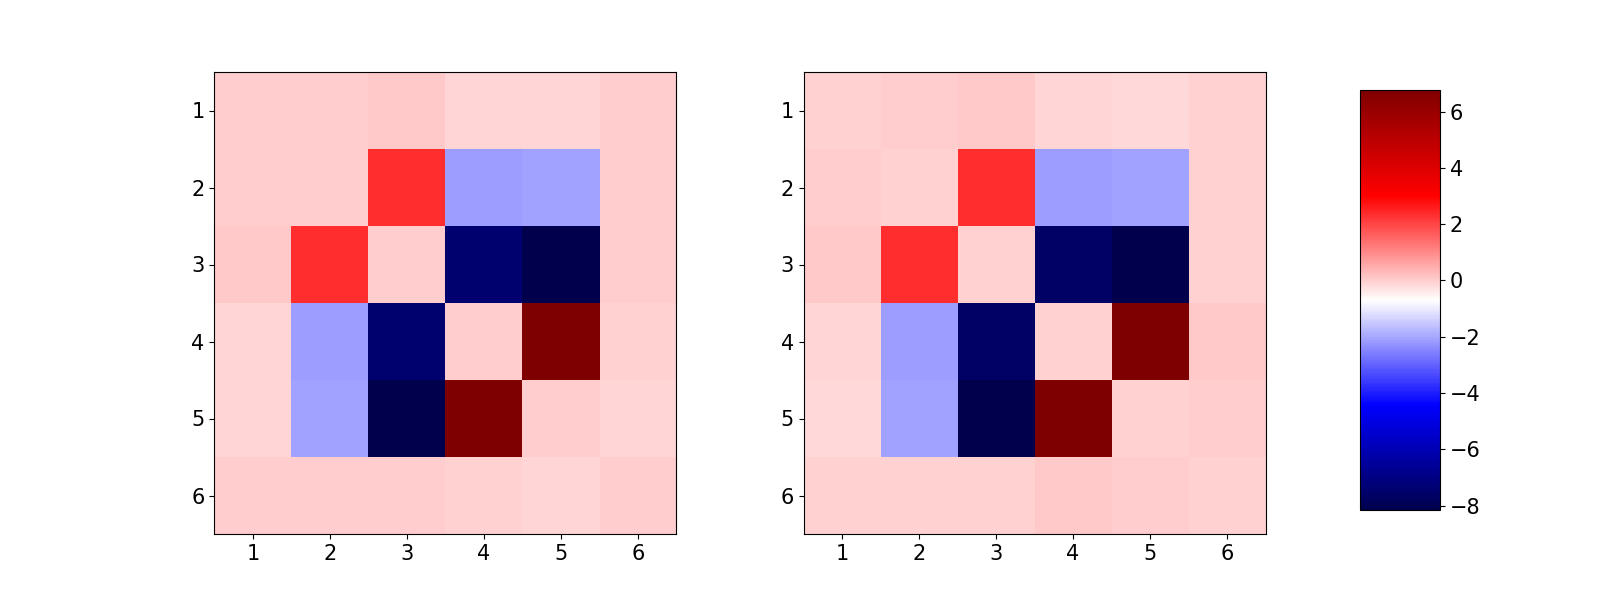
\includegraphics[width=140mm]{plots/yacht_hydrodynamics_posterior_covariance.png} \\
		(c) Comparison of true and estimated posterior covariances \\[6pt] 
	\end{tabular}
	\caption{Comparison of the ground truth posterior of a linear regression model fit to the Yacht Hydrodynamics dataset, and the approximate posterior learned by VIFA. Variances and covariance are plotted separately due to the difference in their magnitude. In plot (c), the diagonal entries of the covariance matrices have been set to zero.}
	\label{fig:posterior_yacht_hydrodynamics}
\end{figure}


\begin{table}[h!]
	\begin{center}
		\begin{tabular}{|| p{0.21\linewidth} p{0.21\linewidth} p{0.21\linewidth} p{0.21\linewidth} ||} 
 			\hline
 			Dataset & Relative Distance from Mean & Relative Distance from Covariance & Scaled Wasserstein Distance \\ [0.5ex] 
 			\hline\hline
			Energy Efficiency 	& 0.0042 	& 0.0765 & 0.0646 \\ 
			\hline
			Boston Housing 	& 0.0253 	& 0.1467 & 0.0333 \\ 
			\hline
			Concrete Strength 	& 0.0058 	& 0.1267 & 0.0477 \\ 
			\hline
 			Yacht Hydro. 		& 0.0437 	& 0.0477 & 0.1113 \\ [1ex] 
			\hline
		\end{tabular}
		\caption{For each UCI dataset, the distance between the true posterior distribution of the parameter vector of a linear regression model and the approximate FA posterior estimated by VIFA. Relative distances between the true and approximate means and covariances are shown. Each relative distance is the Frobenius norm of the difference between the true parameter and the approximate parameter divided by the Frobenius norm of the true parameter. Also shown is the 2-Wasserstein distance between the true posterior Gaussian distribution and the approximate Gaussian distribution, divided by the number of dimensions in the dataset.}
		\label{table:linear_regression_vi_posterior_uci}
	\end{center}
\end{table}


%\section{Making Predictions}
%
%Regardless of whether SWAG does Bayesian inference or not, it was shown in \cite{maddox2019} that this method can lead to more accurate predictions. Once a Gaussian distribution has been learned from the SGD iterates, parameter vectors of the model can easily be sampled. For each sampled parameter vector, the resultant model can be used to make a different set of predictions for the test data. Final predictions are then obtained by averaging the predictions from all models. The aim of the experiments in this section is to test, for linear regression, whether this approach leads to more accurate predictions than standard SGD, when the Gaussian distribution of the parameter vectors is a FA model learned by either online SGA or online EM. 
%
%\subsection{Methodology}
%
%For these experiments, four real regression datasets from the UCI Machine Learning Repository \cite{dua2019} were used. Namely, the Energy Efficiency\footnote{https://archive.ics.uci.edu/ml/datasets/energy+efficiency}, Boston Housing\footnote{https://archive.ics.uci.edu/ml/machine-learning-databases/housing}, Concrete Compressive Strength\footnote{https://archive.ics.uci.edu/ml/datasets/concrete+compressive+strength} and Yacht Hydrodynamics\footnote{http://archive.ics.uci.edu/ml/datasets/yacht+hydrodynamics} datasets. More details about these datasets are given in Table \ref{table:uci_datasets}. Note that the Energy Efficiency dataset has two target variables, heating load and cooling load, but in these experiments only the heating load was used. 
%
%\begin{table}[h!]
%	\begin{center}
%		\begin{tabular}{||c c c ||} 
%			\hline
% 			Dataset & No. of Instances & No. of Input Variables \\ [0.5ex] 
%			\hline\hline
%			Energy Efficiency & 768 & 8 \\
% 			\hline
% 			Boston Housing & 506 & 13 \\ 
% 			\hline
% 			Concrete Compressive Strength & 1030 & 8 \\
% 			\hline
% 			Yacht Hydrodynamics & 308 & 6 \\ [1ex] 
% 			\hline
%		\end{tabular}
%		\caption{UCI regression datasets used in experiments with linear regression.}
%		\label{table:uci_datasets}
%	\end{center}
%\end{table}
%
%For each dataset, the model was pre-trained for 500 epochs of SGD with a learning rate of 0.001, as in the synthetic experiments in Section \ref{sec:linear_regression_posterior_experiments}. Then, starting from the pre-trained model, a further 100 epochs of SGD were executed. During this time, the parameter vectors sampled after each mini-batch gradient update were used to fit two FA models, one via online SGA and another via online EM. For these final 100 epochs, a learning rate of 0.1 and weight decay of 0.001 were used. These hyperparameters were chosen since it was observed in Figure \ref{fig:linear_regression_pdfs} that this setting produced samples most representative of the true posterior for the synthetic data. During the pre-training phase, the weight decay was also set to 0.001 to make for a fairer comparison with the pre-trained model. For all epochs, the batch size was set to one tenth of the size of the full dataset. Both FA models had a latent dimension of three. Following the approach in the experiments in Chapter \ref{ch:online_fa_experiments}, the first 100 sampled parameter vectors were only used to update the running averages, $\overline{\theta}_t, \overline{\matr{A}}_t, \overline{\matr{B}}_t$ and $\overline{\matr{d}^2}_t$, while $\matr{F}$ and $\Psi$ remained fixed. Again, the FA model updated via online SGA used a learning rate of 0.001. After training, test predictions were made using the pre-trained parameter vector, the empirical mean of the sampled parameter vectors, $\theta_{\text{SWA}}$, and two ensembles, one for each FA model. Each ensemble was constructed by sampling 30 parameter vectors from the FA model and averaging the resultant predictions, as in the UCI regression experiments in \cite{maddox2019}. This process was repeated for 10 folds of cross-validation. Within each fold, the input features where standardised why subtracting their mean and dividing by their standard deviation, where these statistics were calculated using the fold's training data only. 
%
%
%\subsection{Results and Discussion}
%
%Figure \ref{fig:linear_regression_mse} shows the average test mean squared error (MSE) for each dataset and prediction method. The average errors were computed over ten folds of cross-validation, and standard error bars are also plotted. Across all datasets, the SWA solution and the FA ensemble learned via online EM are the best prediction methods in general in terms of the average error. These two methods achieved almost identical results on all datasets. On three out of the four datasets they achieve lower average error than the pre-trained solution. The difference is relatively large in the case of the Energy Efficiency dataset, but for all other datasets the standard error bars have significant overlap. Recall that, in the experiments in Chapter \ref{ch:online_fa_experiments}, online EM was better at fitting FA models than online SGA. This appears to translate into more accurate linear regression ensembles, as the average MSE of the online EM ensemble is less than that of the online SGA ensemble for all datasets. The numerical MSE results are also given in Table \ref{table:linear_regression_mse} of the appendix. 
%
%\begin{figure}[!htbp] 
%	\begin{tabular}{cc}
%		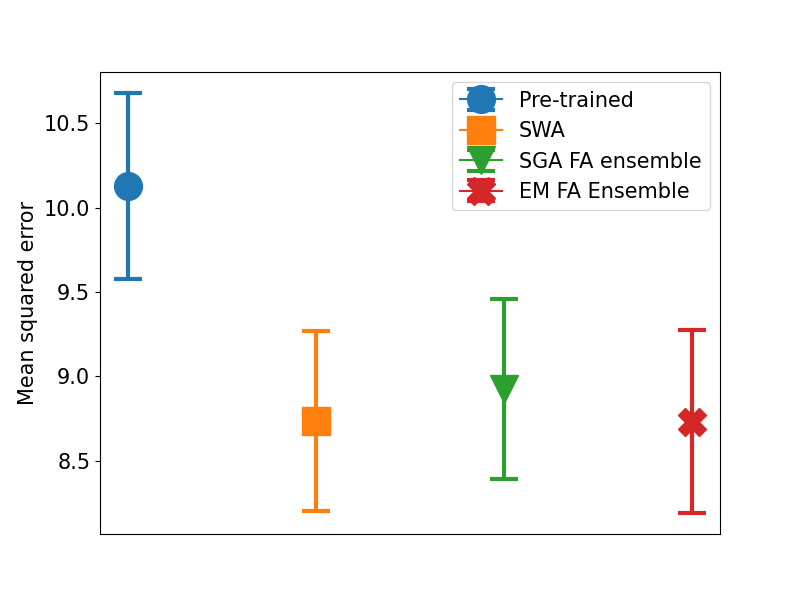
\includegraphics[width=70mm]{plots/linear_regression_predictions_mse__energy_efficiency.png}
%		& 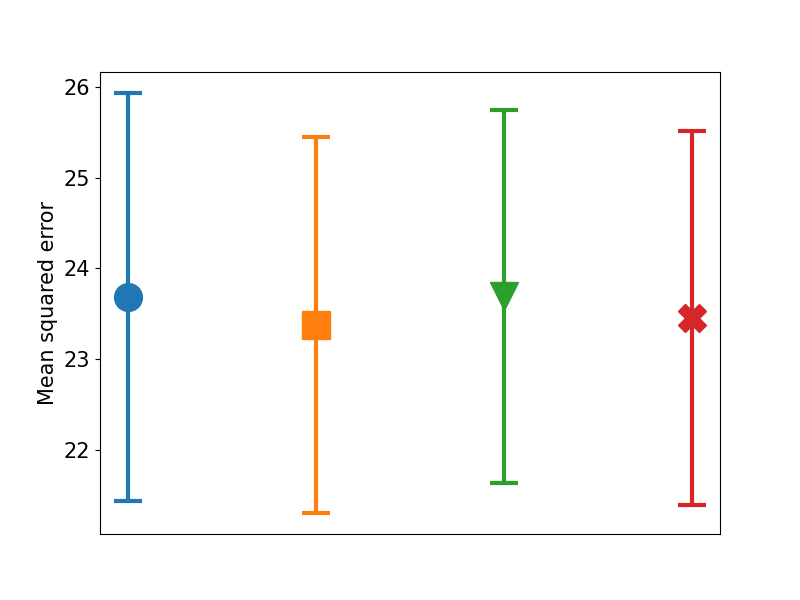
\includegraphics[width=70mm]{plots/linear_regression_predictions_mse__boston_housing.png} \\
%		(a) Energy Efficiency 
%		 & (b) Boston Housing \\[6pt] 
%		 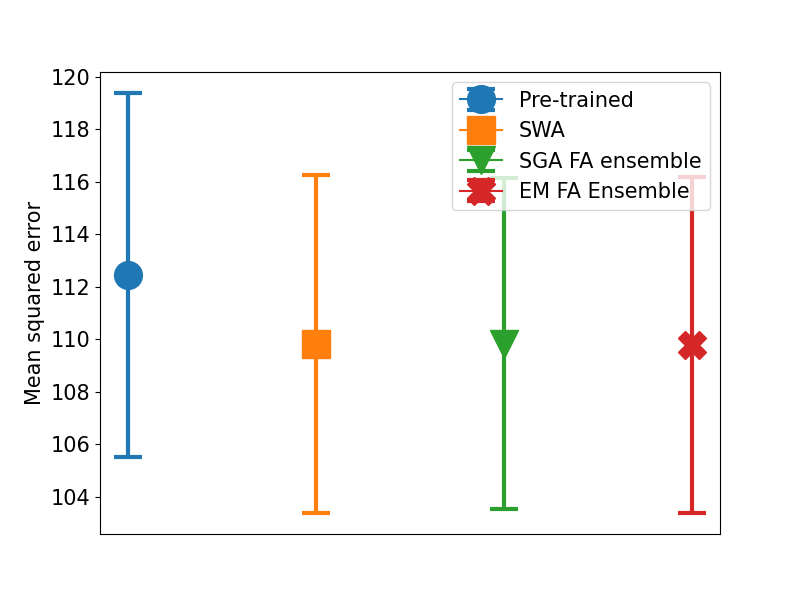
\includegraphics[width=70mm]{plots/linear_regression_predictions_mse__concrete_strength.png} 
%		 & 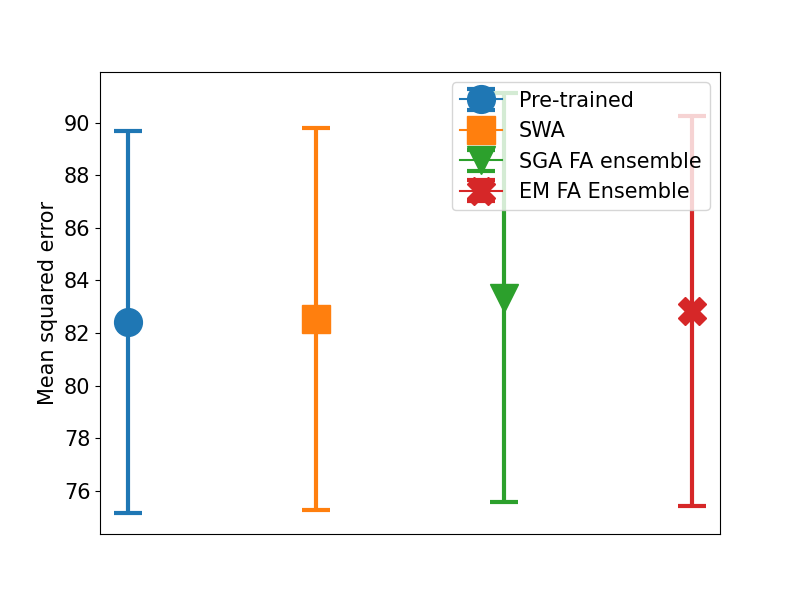
\includegraphics[width=70mm]{plots/linear_regression_predictions_mse__yacht_hydrodynamics.png} \\
%		 (c) Concrete Compressive Strength 
%		 & (d) Yacht Hydrodynamics \\[6pt]
%	\end{tabular}
%	\caption{Average test mean squared error of linear regression models on four UCI regression datasets. Results are show for four different prediction methods: using the pre-trained parameter vector (blue), using the SWA solution (orange) and two ensembles formed by sampling parameter vectors from FA models fit to the SGD iterates, one via online SGA (green) and another learned via online EM (red). The markers show the average test error over ten folds of cross-validation, and standard error bars are also plotted.}
%	\label{fig:linear_regression_mse}
%\end{figure}
%
%These results suggest that, in the case of linear regression, fitting a FA model to the SGD iterates via online EM and then using it to construct an ensemble can lead to more accurate predictions compared to standard SGD. However, this approach does not seem to improve on the much simpler SWA solution. Note that, in the case of linear regression, an ensemble of $M$ parameter vectors sampled from a FA model can be written as 
%\begin{equation}
%	\frac{1}{M} \sum_{m=1}^M \theta_m^\intercal \matr{x} 
%	= \Bigg( \frac{1}{M} \sum_{m=1}^M \theta_m^\intercal \Bigg) \matr{x} 
%	= \theta_{\text{FA}}^\intercal \matr{x}.
%\end{equation}
%Hence, if the learned FA model is a good approximation of the empirical Gaussian distribution of the SGD iterates, $\theta_{\text{FA}}$ will be similar to $\theta_{\text{SWA}}$ for large $M$. This observation and the results in Figure \ref{fig:linear_regression_mse} suggests that, if the accuracy of linear regression predictions is all that matters, the best approach is to use $\theta_{\text{SWA}}$.


%\chapter{Gaussian Processes Experiments}
%
%In was show in Section \ref{sec:gps} that, under certain conditions on the parameters, a neural network with a single, infinitely wide, hidden layer is equivalent to a GP with kernel function $k_{\text{NN}}$ given in Equation (\ref{eqn:nn_kernel}). The kernel depends on $\Sigma_{\matr{w}} \in \R^{D \times D}$, which is the covariance of the prior on the weights of each hidden unit. The individual weights of a neural network are usually independent on initialisation, so $\Sigma_{\matr{w}}$ can be set to a diagonal matrix $\sigma_w \matr{I}$. With this, $k_{\text{NN}}(\matr{x}, \matr{x}')$ can be evaluated for any two points $\matr{x}, \matr{x}' \in \R^D$. Hence, given training inputs $\matr{X} \in \R^{N\times D}$, training outputs $\matr{y} \in \R^N$ and a test point $\matr{x}_{*} \in \R^D$, the Gaussian posterior predictive distribution $p(f_{*} | \matr{X}, \matr{y}, \matr{x}_{*})$ can be computed according to Equation (\ref{eqn:gp_prediction}). 
%
%Alternatively, $p(f_{*} | \matr{X}, \matr{y}, \matr{x}_{*})$ can be estimated via an approximate Bayesian model average (BMA). Given a posterior over the parameters of a neural network, $p(\theta |  \matr{X}, \matr{y})$, a parameter vector $\tilde{\theta} \sim p(\theta |  \matr{X}, \matr{y})$ can be used to construct a specific instance of the neural network and make a prediction for $\matr{x}_{*}$. If this procedure is repeated multiple times, the mean and variance of $p(f_{*} | \matr{X}, \matr{y}, \matr{x}_{*})$ can be estimated and compared directly to the ground truth. To obtain the parameter posterior, the online FA algorithms can be used to fit a Gaussian posterior to the iterates of the parameter vector, $\theta_1, \dots, \theta_T$, encountered while training the single layer neural network via SGD. Of course, in practice it is impossible to train a neural network with an infinitely wide hidden layer, but for these experiments it will suffice to consider neural networks with a few hundred hidden units. 
%
%
%\section{Methodology}
%
%\section{Results}

\chapter{Neural Network Experiments}

Given the encouraging results achieved by VIFA in Chapter \ref{ch:linear_regression_experiments}, the purpose of these experiments is to test VIFA on simple neural networks with a sinlge hidden layer. Unlike linear regression, it is not possible to compute the true posterior distribution of the parameter vector of a non-linear neural network in closed form. Therefore, the focus in these experiments is on the quality of predictions made by neural networks trained via VIFA in comparison to SLANG. Methods based on stochastic weight averaging were excluded due to their poor performance in the experiments in Chapter \ref{ch:linear_regression_experiments}. While poor posterior estimation does not necessarily translate into poor predictions, this project is primarily interested in methods which can be used to construct reliable uncertainty estimates for neural network predictions in addition to point estimates. 

\section{Methodology}

The setup for the experiments largely followed the methodology adopted by the authors of SLANG \cite{mishkin2018}. Each neural network had a single hidden layer with 50 rectified linear units and a single, unactivated output. The UCI regression datasets from Table \ref{table:uci_datasets} were used once again. Each dataset was split 20 times into different train and tests sets\footnote{Data splits are available at \texttt{https://github.com/yaringal/DropoutUncertaintyExps}}. For each train-test split, VIFA hyperparameters were tuned using the training data and then the best configuration was evaluated once on the test set (TODO: haven't touched test sets yet - leaving until the end). The hyperparameters which were tuned were the learning rate $\eta$, the precision $\alpha$ of the prior and the precision $\beta$ of the additive target noise distribution. As with SLANG, these were optimised via 30 iterations of hyperparameter search, with 5-fold cross-validation performed in each iteration to estimate the average negative log-likelihood (ANLL). However, while SLANG used Bayesian optimisation, VIFA was tuned via random search to keep things simple. During the search, values for $\eta$, $\alpha$ and $\beta$ we sampled log-uniformly from $[0.01, 0.02]$, $[0.01, 10]$ and $[0.01, 1]$, respectively. To improve numerical stability, any gradients with Frobenius norm greater than 10 were rescaled to have norm of exactly 10. The other hyperparameters were fixed to the same values as SLANG. That is, latent dimension $K=1$, number of epochs $T=120$, mini-batch size $M=10$ and Monte Carlo average size $L=4$.  Before each training run, the features and target were normalised by subtracting their mean and dividing by their standard deviation. These statistics were computed on training data only, including within each separate fold of cross-validation.  

While training, the ANLL term used on line 12 of Algorithm \ref{alg:vi_fa} was set to
\begin{equation}\label{eqn:train_nll}
	-\frac{1}{M} \sum_{(\matr{x}, y) \in \mathcal{B}} \log \mathcal{N}\big(y; f(\matr{x}; \theta), \beta^{-1}\big),
\end{equation}
where $\mathcal{B}$ is a mini-batch of $M$ training examples and $f(\matr{x}; \theta)$ is the prediction of the neural network for input $\matr{x}$ and parameters $\theta$. When evaluating, the ANLL was computed slightly differently. First, 10 separate parameter vectors were sampled for the neural network and used to make predictions for each input. The predictions were un-normalised to return them to their original scale. Next, for each input $\matr{x}$, the mean and variance of the 10 predictions were computed, say $\mu_\matr{x}$ and $\sigma_\matr{x}^2$, respectively. Then the ANLL for a set of $N$ validation or test points $\mathcal{D}$ was set to
\begin{equation}\label{eqn:test_nll}
	-\frac{1}{N} \sum_{(\matr{x}, y) \in \mathcal{D}} \log \mathcal{N}\big(y; \mu_\matr{x},\sigma_\matr{x}^2\big).
\end{equation}
In addition, the root mean square error (RMSE) between the predicted means $\mu_\matr{x}$ and the targets $y$ was also calculated.

Although \cite{mishkin2018} provides these metrics for SLANG, the experiments were re-run\footnote{Using the code available at \texttt{https://github.com/aaronpmishkin/SLANG}} with some adjustments to allow for a fairer comparison with VIFA. In particular, when the authors of SLANG compute the validation and test ANLL, they use the function
\begin{equation}\label{eqn:slang_nll}
	-\frac{1}{N} \sum_{(\matr{x}, y) \in \mathcal{D}} \log \mathcal{N}\big(y; \mu_\matr{x},\beta^{-1}\big).
\end{equation}
This does not seem fair, since $\beta$ is a tuned hyperparameter. It should not affect the validation and test metrics directly. Therefore, the ANLL calculation in their code was modified to match that of VIFA. That is, Equation (\ref{eqn:test_nll}). Finally, the hyperparameter ranges for $\alpha$ and $\beta$ were adjusted to also match those of VIFA. 


\section{Results and Discussion} 

Test metrics from VIFA and SLANG are given in Table \ref{table:neural_nets_uci} (TODO: these are actually validation metrics for now - swap for test at the end). As well as the results for neural networks, prediction metrics for VIFA applied to linear regression are also given. 

\begin{table}[h!]
	\begin{center}
		\begin{tabular}{|| p{0.13\linewidth} p{0.21\linewidth} p{0.15\linewidth} p{0.15\linewidth} p{0.23\linewidth} ||} 
 			\hline
 			Metric & Dataset & VIFA-LR & VIFA-NN & SLANG-NN \\ [0.5ex] 
 			\hline\hline
			ANLL 	& Energy Efficiency 	& $\mathbf{2.80 \pm 0.03}$  	& $2.87 \pm 0.03$ 			& $>10,000$ \\ 
					& Boston Housing 	& $3.07 \pm 0.02$ 			& $\mathbf{2.99 \pm 0.01}$ 	& $>10,000$ \\ 
					& Concrete Strength & $\mathbf{3.87 \pm 0.01}$ 	& $4.61 \pm 0.16$ 			& $>10,000$ \\ 
 					& Yacht Hydro. 		& $3.76 \pm 0.01$ 			& $\mathbf{2.55 \pm 0.03}$ 	& $35.65 \pm 10.98$ \\
 			\hline
			RMSE 	& Energy Efficiency 	& $\mathbf{3.30 \pm 0.05}$  	& $\mathbf{3.33 \pm 0.05}$ 	& $414.78 \pm 397.33$ \\ 
					& Boston Housing 	& $5.36 \pm 0.10$ 			& $\mathbf{4.97 \pm 0.07}$ 	& $12.89 \pm 6.88$ \\ 
					& Concrete Strength & $11.40 \pm 0.11$ 			& $\mathbf{7.43 \pm 0.06}$ 	& $12.96 \pm 4.52$ \\ 
 					& Yacht Hydro. 		& $9.64 \pm 0.05$ 			& $3.32 \pm 0.07$ 			& $\mathbf{2.24 \pm 0.72}$ 
					\\ [1ex] 
			\hline
		\end{tabular}
		\caption{Test results for prediction experiments with UCI regression datasets. LR and NN refer to linear regression and neural network, respectively. Average test metrics over 20 different train-test splits are given, along with standard errors.}
		\label{table:neural_nets_uci}
	\end{center}
\end{table}



\chapter{Conclusions}

\section{Final Reminder}

The body of your dissertation, before the references and any appendices,
\emph{must} finish by page~40. The introduction, after preliminary material,
should have started on page~1.

You may not change the dissertation format (e.g., reduce the font
size, change the margins, or reduce the line spacing from the default
1.5 spacing). Over length or incorrectly-formatted dissertations will
not be accepted and you would have to modify your dissertation and
resubmit.  You cannot assume we will check your submission before the
final deadline and if it requires resubmission after the deadline to
conform to the page and style requirements you will be subject to the
usual late penalties based on your final submission time.

\bibliographystyle{plain}
\bibliography{main}

% You can include appendices like this:
 \appendix

 \chapter{Supplementary Results}
 
 \section{Online Factor Analysis}
 
Tables \ref{table:fa_covar_distance} and \ref{table:fa_wasserstein} contain the numerical results corresponding to the data plotted in  Figures \ref{fig:fa_covar_distance} and \ref{fig:fa_wasserstein}, respectively, for the case of 100,000 training samples. 
 
\begin{table}[h!]
	\begin{center}
		\begin{tabular}{|| p{0.12\linewidth} p{0.20\linewidth} p{0.20\linewidth} p{0.20\linewidth} p{0.20\linewidth} ||} 
 			\hline
 			Obs. Dim & Spectrum Range & Batch SVD & Online EM & Online SGA \\ [0.5ex] 
 			\hline\hline
			100 	& $[1, 10]$ 	& $0.0454 \pm 0.0077$ 	& $0.0399 \pm 0.0058$	& $0.0426 \pm 0.0005$ \\ 
				& $[1, 100]$ 	& $0.0631 \pm 0.0073$ 	& $0.0613 \pm 0.0057$ 	& $0.1309 \pm 0.0038$ \\ 
				& $[1, 1000]$	& $0.0608 \pm 0.0087$ 	& $0.1767 \pm 0.0037$ 	& $0.2350 \pm 0.0046$ \\ 
			\hline
			1000	& $[1, 10]$ 	& $0.0204 \pm 0.0010$ 	& $0.0207 \pm 0.0003$ 	& $0.0546 \pm 0.0009$ \\ 
				& $[1, 100]$ 	& $0.0217 \pm 0.0011$ 	& $0.0238 \pm 0.0013$ 	& $0.0472 \pm 0.0008$ \\ 
				& $[1, 1000]$ 	& $0.0218 \pm 0.0011$ 	& $0.0501 \pm 0.0016$ 	& $0.0945 \pm 0.0024$ \\ [1ex] 
			\hline
		\end{tabular}
		\caption{The relative distance of the estimated FA covariance matrix from the true covariance matrix when the latent dimension of the FA model is 10 and the number of training samples is 100,000. The relative distance is the Frobenius norm of the difference between the true covariance matrix and the estimated covariance matrix divided by the Frobenius norm of the true covariance matrix. Each result is the mean value over ten trials with different random seeds, along with standard errors. These results correspond to the rightmost points in the plots in Figure \ref{fig:fa_covar_distance}.}
		\label{table:fa_covar_distance}
	\end{center}
\end{table}

\begin{table}[h!]
	\begin{center}
		\begin{tabular}{|| p{0.12\linewidth} p{0.20\linewidth} p{0.20\linewidth} p{0.20\linewidth} p{0.20\linewidth} ||} 
 			\hline
 			Obs. Dim & Spectrum Range & Batch SVD & Online EM & Online SGA \\ [0.5ex] 
 			\hline\hline
			100 	& $[1, 10]$ 	& $0.0061 \pm 0.0009$ 	& $0.0058 \pm 0.0006$ 	& $0.0062 \pm 0.0004$ \\ 
				& $[1, 100]$ 	& $0.0256 \pm 0.0022$ 	& $0.0246 \pm 0.0021$ 	& $0.0446 \pm 0.0018$ \\ 
				& $[1, 1000]$	& $0.0780 \pm 0.0089$ 	& $0.2137 \pm 0.0054$ 	& $0.2855 \pm 0.0040$ \\ 
			\hline
			1000	& $[1, 10]$ 	& $0.0015 \pm 0.0001$ 	& $0.0016 \pm 0.0001$ 	& $0.0023 \pm 0.0001$ \\ 
				& $[1, 100]$ 	& $0.0048 \pm 0.0002$ 	& $0.0049 \pm 0.0002$ 	& $0.0062 \pm 0.0001$ \\ 
				& $[1, 1000]$ 	& $0.0152 \pm 0.0005$ 	& $0.0217 \pm 0.0003$ 	& $0.0349 \pm 0.0006$ \\ [1ex] 
			\hline
		\end{tabular}
		\caption{The 2-Wasserstein distance between the Gaussian distribution defined by the estimated FA model and the Gaussian distribution defined by the true FA model, divided by the observation dimension, when the latent dimension of the FA model is 10 and the number of training samples is 100,000. Each result is the mean value over ten trials with different random seeds, along with standard errors. These results correspond to the rightmost points in the plots in Figure \ref{fig:fa_wasserstein}.}
		\label{table:fa_wasserstein}
	\end{center}
\end{table}


% \section{Linear Regression Predictions}\label{appendix:linear_regression_predictions}
% 
% Table \ref{table:linear_regression_mse} contains the same results as Figure \ref{fig:linear_regression_mse}, but in tabular format.  
% 
% \begin{table}[h!]
%	\begin{center}
%		\begin{tabular}{|| p{0.21\linewidth} p{0.16\linewidth} p{0.16\linewidth} p{0.16\linewidth} p{0.16\linewidth} ||} 
% 			\hline
% 			Dataset & Pre-trained & SWA & SGA-FA & EM-FA \\ [0.5ex] 
% 			\hline\hline
%			Energy Efficiency & $10.13 \pm 0.55$ & $8.74 \pm 0.54$ & $8.93 \pm 0.53$ & $\bf{8.73 \pm 0.54}$ \\
%			Boston Housing & $23.69 \pm 2.25$ & $\bf{23.27 \pm 2.07}$ & $23.69 \pm 2.06$ & $23.46 \pm 2.06$ \\
%			Concrete Strength & $112.44 \pm 6.93$ & $109.83 \pm 6.44$ & $109.84 \pm 6.30$ & $\bf{109.79 \pm 6.41}$ \\
%			Yacht Hydro. & $\bf{82.43 \pm 7.28}$ & $82.54 \pm 7.27$ & $83.35 \pm 7.78$ & $82.83 \pm 7.42$ \\ [1ex] 
%			\hline
%		\end{tabular}
%		\caption{Average test mean squared error of linear regression models on four UCI regression datasets. Results are show for four different prediction methods: using the pre-trained parameter vector (second column), using the SWA solution (third column) and two ensembles formed by sampling parameter vectors from FA models fit to the SGD iterates, one via online SGA (fourth column) and another learned via online EM (fifth column). Results are average over ten folds of cross-validation, and standard errors are also given. Bold text highlights the lowest average error for each dataset, without taking into account the standard errors.}
%		\label{table:linear_regression_mse}
%	\end{center}
%\end{table}



\end{document}